\documentclass[a4paper]{book}
\usepackage{a4wide}
\usepackage{makeidx}
\usepackage{fancyhdr}
\usepackage{graphicx}
\usepackage{multicol}
\usepackage{float}
\usepackage{textcomp}
\usepackage{alltt}
\usepackage{times}
\usepackage{ifpdf}
\ifpdf
\usepackage[pdftex,
            pagebackref=true,
            colorlinks=true,
            linkcolor=blue
           ]{hyperref}
\else
\usepackage[ps2pdf,
            pagebackref=true,
            colorlinks=true,
            linkcolor=blue
           ]{hyperref}
\usepackage{pspicture}
\fi
\usepackage{doxygen}
\makeindex
\setcounter{tocdepth}{1}
\renewcommand{\footrulewidth}{0.4pt}
\begin{document}
\begin{titlepage}
\vspace*{7cm}
\begin{center}
{\Large Paradis\-EO-PEOMoving\-Objects Reference Manual\\[1ex]\large 1.0 }\\
\vspace*{1cm}
{\large Generated by Doxygen 1.4.7}\\
\vspace*{0.5cm}
{\small Mon Oct 8 11:16:45 2007}\\
\end{center}
\end{titlepage}
\clearemptydoublepage
\pagenumbering{roman}
\tableofcontents
\clearemptydoublepage
\pagenumbering{arabic}
\chapter{The Paradis\-EO-PEO Framework }
\label{index}\hypertarget{index}{}\section{Introduction}\label{main_Introduction}
The capacitated vehicle routing problem with time windows or CVRP-TW is a combinatorial optimization problem seeking to service a number of customers with a fleet of vehicles where the vehicles have a mimited capacity and the delivery locations have time windows within which the deliveries (or visits) must be made. Often the context is that of delivering goods located at a central depot to customers who have placed orders for such goods. Implicit is the goal of minimizing the cost of distributing the goods. Finding the global minimum for the cost function, except for the smallest instances, is computationally complex.\section{AUTHORS}\label{main_authors}
\begin{TabularC}{3}
\hline
Dolphin project-team INRIA Futurs, 2007. &Antonio La\-Torre atorre[at]fi.upm.es &Thomas Legrand paradiseo-help[at]lists.gforge.inria.fr  \\\hline
\end{TabularC}
\section{LICENSE}\label{main_LICENSE}
This software is governed by the Ce\-CILL license under French law and abiding by the rules of distribution of free software. You can use, modify and/ or redistribute the software under the terms of the Ce\-CILL license as circulated by CEA, CNRS and INRIA at the following URL \char`\"{}http://www.cecill.info\char`\"{}.

As a counterpart to the access to the source code and rights to copy, modify and redistribute granted by the license, users are provided only with a limited warranty and the software's author, the holder of the economic rights, and the successive licensors have only limited liability.

In this respect, the user's attention is drawn to the risks associated with loading, using, modifying and/or developing or reproducing the software by the user in light of its specific status of free software, that may mean that it is complicated to manipulate, and that also therefore means that it is reserved for developers and experienced professionals having in-depth computer knowledge. Users are therefore encouraged to load and test the software's suitability as regards their requirements in conditions enabling the security of their systems and/or data to be ensured and, more generally, to use and operate it in the same conditions as regards security. The fact that you are presently reading this means that you have had knowledge of the Ce\-CILL license and that you accept its terms.

Paradis\-EO Web\-Site : \tt{http://paradiseo.gforge.inria.fr} Contact: \tt{paradiseo-help@lists.gforge.inria.fr}\section{Home Page}\label{main_Paradiseo}
{\tt http://paradiseo.gforge.inria.fr} 
\chapter{Paradis\-EO-PEOMoving\-Objects Namespace Index}
\section{Paradis\-EO-PEOMoving\-Objects Namespace List}
Here is a list of all documented namespaces with brief descriptions:\begin{CompactList}
\item\contentsline{section}{\hyperlink{namespacepeo}{peo} }{\pageref{namespacepeo}}{}
\end{CompactList}

\chapter{Paradis\-EO-PEOMoving\-Objects Hierarchical Index}
\section{Paradis\-EO-MO-Moving\-Objects Class Hierarchy}
This inheritance list is sorted roughly, but not completely, alphabetically:\begin{CompactList}
\item \contentsline{section}{mo\-Algo$<$ EOT $>$}{\pageref{classmo_algo}}{}
\item \contentsline{section}{mo\-Aspir\-Crit$<$ M $>$}{\pageref{classmo_aspir_crit}}{}
\begin{CompactList}
\item \contentsline{section}{mo\-Impr\-Best\-Fit\-Aspir\-Crit$<$ M $>$}{\pageref{classmo_impr_best_fit_aspir_crit}}{}
\item \contentsline{section}{mo\-No\-Aspir\-Crit$<$ M $>$}{\pageref{classmo_no_aspir_crit}}{}
\end{CompactList}
\item \contentsline{section}{mo\-Comparator$<$ EOT $>$}{\pageref{classmo_comparator}}{}
\begin{CompactList}
\item \contentsline{section}{mo\-Fit\-Comparator$<$ EOT $>$}{\pageref{classmo_fit_comparator}}{}
\end{CompactList}
\item \contentsline{section}{mo\-Cooling\-Schedule}{\pageref{classmo_cooling_schedule}}{}
\begin{CompactList}
\item \contentsline{section}{mo\-Exponential\-Cooling\-Schedule}{\pageref{classmo_exponential_cooling_schedule}}{}
\item \contentsline{section}{mo\-Linear\-Cooling\-Schedule}{\pageref{classmo_linear_cooling_schedule}}{}
\end{CompactList}
\item \contentsline{section}{mo\-HC$<$ M $>$}{\pageref{classmo_h_c}}{}
\item \contentsline{section}{mo\-ILS$<$ M $>$}{\pageref{classmo_i_l_s}}{}
\item \contentsline{section}{mo\-LSCheck\-Point$<$ M $>$}{\pageref{classmo_l_s_check_point}}{}
\item \contentsline{section}{mo\-Move$<$ EOT $>$}{\pageref{classmo_move}}{}
\item \contentsline{section}{mo\-Move\-Expl$<$ M $>$}{\pageref{classmo_move_expl}}{}
\begin{CompactList}
\item \contentsline{section}{mo\-Move\-Loop\-Expl$<$ M $>$}{\pageref{classmo_move_loop_expl}}{}
\begin{CompactList}
\item \contentsline{section}{mo\-HCMove\-Loop\-Expl$<$ M $>$}{\pageref{classmo_h_c_move_loop_expl}}{}
\item \contentsline{section}{mo\-TSMove\-Loop\-Expl$<$ M $>$}{\pageref{classmo_t_s_move_loop_expl}}{}
\end{CompactList}
\end{CompactList}
\item \contentsline{section}{mo\-Move\-Incr\-Eval$<$ M $>$}{\pageref{classmo_move_incr_eval}}{}
\item \contentsline{section}{mo\-Move\-Init$<$ M $>$}{\pageref{classmo_move_init}}{}
\item \contentsline{section}{mo\-Move\-Select$<$ M $>$}{\pageref{classmo_move_select}}{}
\begin{CompactList}
\item \contentsline{section}{mo\-Best\-Impr\-Select$<$ M $>$}{\pageref{classmo_best_impr_select}}{}
\item \contentsline{section}{mo\-First\-Impr\-Select$<$ M $>$}{\pageref{classmo_first_impr_select}}{}
\item \contentsline{section}{mo\-Rand\-Impr\-Select$<$ M $>$}{\pageref{classmo_rand_impr_select}}{}
\end{CompactList}
\item \contentsline{section}{mo\-Next\-Move$<$ M $>$}{\pageref{classmo_next_move}}{}
\begin{CompactList}
\item \contentsline{section}{mo\-It\-Rand\-Next\-Move$<$ M $>$}{\pageref{classmo_it_rand_next_move}}{}
\end{CompactList}
\item \contentsline{section}{mo\-Rand\-Move$<$ M $>$}{\pageref{classmo_rand_move}}{}
\item \contentsline{section}{mo\-SA$<$ M $>$}{\pageref{classmo_s_a}}{}
\item \contentsline{section}{mo\-Sol\-Continue$<$ EOT $>$}{\pageref{classmo_sol_continue}}{}
\begin{CompactList}
\item \contentsline{section}{mo\-Fit\-Sol\-Continue$<$ EOT $>$}{\pageref{classmo_fit_sol_continue}}{}
\item \contentsline{section}{mo\-Gen\-Sol\-Continue$<$ EOT $>$}{\pageref{classmo_gen_sol_continue}}{}
\item \contentsline{section}{mo\-No\-Fit\-Impr\-Sol\-Continue$<$ EOT $>$}{\pageref{classmo_no_fit_impr_sol_continue}}{}
\item \contentsline{section}{mo\-Steady\-Fit\-Sol\-Continue$<$ EOT $>$}{\pageref{classmo_steady_fit_sol_continue}}{}
\end{CompactList}
\item \contentsline{section}{mo\-Tabu\-List$<$ M $>$}{\pageref{classmo_tabu_list}}{}
\begin{CompactList}
\item \contentsline{section}{mo\-Simple\-Move\-Tabu\-List$<$ M $>$}{\pageref{classmo_simple_move_tabu_list}}{}
\item \contentsline{section}{mo\-Simple\-Solution\-Tabu\-List$<$ M $>$}{\pageref{classmo_simple_solution_tabu_list}}{}
\end{CompactList}
\item \contentsline{section}{mo\-TS$<$ M $>$}{\pageref{classmo_t_s}}{}
\end{CompactList}

\chapter{Paradis\-EO-PEOMoving\-Objects Class Index}
\section{Paradis\-EO-PEO-Parallelanddistributed\-Evolving\-Objects Class List}
Here are the classes, structs, unions and interfaces with brief descriptions:\begin{CompactList}
\item\contentsline{section}{\hyperlink{structAlgorithm}{Algorithm} }{\pageref{structAlgorithm}}{}
\item\contentsline{section}{\hyperlink{classCitySwap}{City\-Swap} (Its swaps two vertices randomly choosen )}{\pageref{classCitySwap}}{}
\item\contentsline{section}{\hyperlink{classCommunicable}{Communicable} }{\pageref{classCommunicable}}{}
\item\contentsline{section}{\hyperlink{classCommunicator}{Communicator} }{\pageref{classCommunicator}}{}
\item\contentsline{section}{\hyperlink{classCompleteTopology}{Complete\-Topology} }{\pageref{classCompleteTopology}}{}
\item\contentsline{section}{\hyperlink{classcontinuator}{continuator} (Abstract class for a continuator within the exchange of data by migration )}{\pageref{classcontinuator}}{}
\item\contentsline{section}{\hyperlink{classCooperative}{Cooperative} }{\pageref{classCooperative}}{}
\item\contentsline{section}{\hyperlink{classDisplayBestRoute}{Display\-Best\-Route} }{\pageref{classDisplayBestRoute}}{}
\item\contentsline{section}{\hyperlink{classEdgeXover}{Edge\-Xover} (Edge Crossover )}{\pageref{classEdgeXover}}{}
\item\contentsline{section}{\hyperlink{classeoContinuator}{eo\-Continuator$<$ EOT $>$} (Specific class for a continuator within the exchange of migration of a population )}{\pageref{classeoContinuator}}{}
\item\contentsline{section}{\hyperlink{classeoReplace}{eo\-Replace$<$ EOT, TYPE $>$} (Specific class for a replacement within the exchange of migration of a population )}{\pageref{classeoReplace}}{}
\item\contentsline{section}{\hyperlink{classeoSelector}{eo\-Selector$<$ EOT, TYPE $>$} (Specific class for a selector within the exchange of migration of a population )}{\pageref{classeoSelector}}{}
\item\contentsline{section}{\hyperlink{classeoSyncContinue}{eo\-Sync\-Continue} (Class for a continuator within the exchange of data by synchrone migration )}{\pageref{classeoSyncContinue}}{}
\item\contentsline{section}{\hyperlink{classMergeRouteEval}{Merge\-Route\-Eval} }{\pageref{classMergeRouteEval}}{}
\item\contentsline{section}{\hyperlink{classMPIThreadedEnv}{MPIThreaded\-Env} }{\pageref{classMPIThreadedEnv}}{}
\item\contentsline{section}{\hyperlink{classOrderXover}{Order\-Xover} (Order Crossover )}{\pageref{classOrderXover}}{}
\item\contentsline{section}{\hyperlink{classPartialMappedXover}{Partial\-Mapped\-Xover} (Partial Mapped Crossover )}{\pageref{classPartialMappedXover}}{}
\item\contentsline{section}{\hyperlink{classPartRouteEval}{Part\-Route\-Eval} (Route Evaluator )}{\pageref{classPartRouteEval}}{}
\item\contentsline{section}{\hyperlink{classpeoAggEvalFunc}{peo\-Agg\-Eval\-Func$<$ EOT $>$} (The \hyperlink{classpeoAggEvalFunc}{peo\-Agg\-Eval\-Func} class offers only the interface for creating aggregate evaluation functions - there are no direct internal functions provided )}{\pageref{classpeoAggEvalFunc}}{}
\item\contentsline{section}{\hyperlink{classpeoAsyncIslandMig}{peo\-Async\-Island\-Mig$<$ TYPESELECT, TYPEREPLACE $>$} (Specific class for a asynchronous migration )}{\pageref{classpeoAsyncIslandMig}}{}
\item\contentsline{section}{\hyperlink{structpeoEvalFunc}{peo\-Eval\-Func$<$ EOT, Fit\-T, Function\-Arg $>$} (Specific class for evaluation )}{\pageref{structpeoEvalFunc}}{}
\item\contentsline{section}{\hyperlink{classpeoGlobalBestVelocity}{peo\-Global\-Best\-Velocity$<$ POT $>$} (Specific class for a replacement thanks to the velocity migration of a population of a PSO )}{\pageref{classpeoGlobalBestVelocity}}{}
\item\contentsline{section}{\hyperlink{classpeoMultiStart}{peo\-Multi\-Start$<$ Entity\-Type $>$} (Class allowing the launch of several algorithms )}{\pageref{classpeoMultiStart}}{}
\item\contentsline{section}{\hyperlink{structpeoMultiStart_1_1AbstractAggregationAlgorithm}{peo\-Multi\-Start$<$ Entity\-Type $>$::Abstract\-Aggregation\-Algorithm} }{\pageref{structpeoMultiStart_1_1AbstractAggregationAlgorithm}}{}
\item\contentsline{section}{\hyperlink{structpeoMultiStart_1_1AbstractAlgorithm}{peo\-Multi\-Start$<$ Entity\-Type $>$::Abstract\-Algorithm} }{\pageref{structpeoMultiStart_1_1AbstractAlgorithm}}{}
\item\contentsline{section}{\hyperlink{structpeoMultiStart_1_1AbstractDataType}{peo\-Multi\-Start$<$ Entity\-Type $>$::Abstract\-Data\-Type} }{\pageref{structpeoMultiStart_1_1AbstractDataType}}{}
\item\contentsline{section}{\hyperlink{structpeoMultiStart_1_1AggregationAlgorithm}{peo\-Multi\-Start$<$ Entity\-Type $>$::Aggregation\-Algorithm$<$ Aggregation\-Algorithm\-Type $>$} }{\pageref{structpeoMultiStart_1_1AggregationAlgorithm}}{}
\item\contentsline{section}{\hyperlink{structpeoMultiStart_1_1Algorithm}{peo\-Multi\-Start$<$ Entity\-Type $>$::Algorithm$<$ Algorithm\-Type $>$} }{\pageref{structpeoMultiStart_1_1Algorithm}}{}
\item\contentsline{section}{\hyperlink{structpeoMultiStart_1_1DataType}{peo\-Multi\-Start$<$ Entity\-Type $>$::Data\-Type$<$ Type $>$} }{\pageref{structpeoMultiStart_1_1DataType}}{}
\item\contentsline{section}{\hyperlink{structpeoMultiStart_1_1FunctionAlgorithm}{peo\-Multi\-Start$<$ Entity\-Type $>$::Function\-Algorithm$<$ Algorithm\-Return\-Type, Algorithm\-Data\-Type $>$} }{\pageref{structpeoMultiStart_1_1FunctionAlgorithm}}{}
\item\contentsline{section}{\hyperlink{structpeoMultiStart_1_1NoAggregationFunction}{peo\-Multi\-Start$<$ Entity\-Type $>$::No\-Aggregation\-Function} }{\pageref{structpeoMultiStart_1_1NoAggregationFunction}}{}
\item\contentsline{section}{\hyperlink{classpeoNoAggEvalFunc}{peo\-No\-Agg\-Eval\-Func$<$ EOT $>$} (The \hyperlink{classpeoNoAggEvalFunc}{peo\-No\-Agg\-Eval\-Func} class does nothing more than an association between a fitness value and a specified individual )}{\pageref{classpeoNoAggEvalFunc}}{}
\item\contentsline{section}{\hyperlink{classpeoPopEval}{peo\-Pop\-Eval$<$ EOT $>$} (Parallel evaluation functor wrapper )}{\pageref{classpeoPopEval}}{}
\item\contentsline{section}{\hyperlink{classpeoPSOSelect}{peo\-PSOSelect$<$ POT $>$} (Specific class for a selection of a population of a PSO )}{\pageref{classpeoPSOSelect}}{}
\item\contentsline{section}{\hyperlink{classpeoSyncIslandMig}{peo\-Sync\-Island\-Mig$<$ TYPESELECT, TYPEREPLACE $>$} (Specific class for a synchronous migration )}{\pageref{classpeoSyncIslandMig}}{}
\item\contentsline{section}{\hyperlink{classpeoTransform}{peo\-Transform$<$ EOT $>$} (Class for a parallel transform )}{\pageref{classpeoTransform}}{}
\item\contentsline{section}{\hyperlink{classpeoWorstPositionReplacement}{peo\-Worst\-Position\-Replacement$<$ POT $>$} (Specific class for a replacement of a population of a PSO )}{\pageref{classpeoWorstPositionReplacement}}{}
\item\contentsline{section}{\hyperlink{classpeoWrapper}{peo\-Wrapper} (Specific class for wrapping )}{\pageref{classpeoWrapper}}{}
\item\contentsline{section}{\hyperlink{structpeoWrapper_1_1AbstractAlgorithm}{peo\-Wrapper::Abstract\-Algorithm} }{\pageref{structpeoWrapper_1_1AbstractAlgorithm}}{}
\item\contentsline{section}{\hyperlink{structpeoWrapper_1_1Algorithm}{peo\-Wrapper::Algorithm$<$ Algorithm\-Type, Algorithm\-Data\-Type $>$} }{\pageref{structpeoWrapper_1_1Algorithm}}{}
\item\contentsline{section}{\hyperlink{structpeoWrapper_1_1Algorithm_3_01AlgorithmType_00_01void_01_4}{peo\-Wrapper::Algorithm$<$ Algorithm\-Type, void $>$} }{\pageref{structpeoWrapper_1_1Algorithm_3_01AlgorithmType_00_01void_01_4}}{}
\item\contentsline{section}{\hyperlink{structpeoWrapper_1_1FunctionAlgorithm}{peo\-Wrapper::Function\-Algorithm$<$ Algorithm\-Return\-Type, Algorithm\-Data\-Type $>$} }{\pageref{structpeoWrapper_1_1FunctionAlgorithm}}{}
\item\contentsline{section}{\hyperlink{structpeoWrapper_1_1FunctionAlgorithm_3_01AlgorithmReturnType_00_01void_01_4}{peo\-Wrapper::Function\-Algorithm$<$ Algorithm\-Return\-Type, void $>$} }{\pageref{structpeoWrapper_1_1FunctionAlgorithm_3_01AlgorithmReturnType_00_01void_01_4}}{}
\item\contentsline{section}{\hyperlink{classRandomTopology}{Random\-Topology} }{\pageref{classRandomTopology}}{}
\item\contentsline{section}{\hyperlink{classReactiveThread}{Reactive\-Thread} }{\pageref{classReactiveThread}}{}
\item\contentsline{section}{\hyperlink{classreplacement}{replacement$<$ TYPE $>$} (Abstract class for a replacement within the exchange of data by migration )}{\pageref{classreplacement}}{}
\item\contentsline{section}{\hyperlink{classRingTopology}{Ring\-Topology} }{\pageref{classRingTopology}}{}
\item\contentsline{section}{\hyperlink{classRouteEval}{Route\-Eval} }{\pageref{classRouteEval}}{}
\item\contentsline{section}{\hyperlink{classRouteInit}{Route\-Init} }{\pageref{classRouteInit}}{}
\item\contentsline{section}{\hyperlink{classRunner}{Runner} }{\pageref{classRunner}}{}
\item\contentsline{section}{\hyperlink{classselector}{selector$<$ TYPE $>$} (Abstract class for a selector within the exchange of data by migration )}{\pageref{classselector}}{}
\item\contentsline{section}{\hyperlink{structSEND__REQUEST}{SEND\_\-REQUEST} }{\pageref{structSEND__REQUEST}}{}
\item\contentsline{section}{\hyperlink{classService}{Service} }{\pageref{classService}}{}
\item\contentsline{section}{\hyperlink{classStarTopology}{Star\-Topology} }{\pageref{classStarTopology}}{}
\item\contentsline{section}{\hyperlink{structSyncCompare}{Sync\-Compare} }{\pageref{structSyncCompare}}{}
\item\contentsline{section}{\hyperlink{structSyncEntry}{Sync\-Entry} }{\pageref{structSyncEntry}}{}
\item\contentsline{section}{\hyperlink{classThread}{Thread} }{\pageref{classThread}}{}
\item\contentsline{section}{\hyperlink{classTopology}{Topology} }{\pageref{classTopology}}{}
\item\contentsline{section}{\hyperlink{classTwoOpt}{Two\-Opt} }{\pageref{classTwoOpt}}{}
\item\contentsline{section}{\hyperlink{classTwoOptIncrEval}{Two\-Opt\-Incr\-Eval} }{\pageref{classTwoOptIncrEval}}{}
\item\contentsline{section}{\hyperlink{classTwoOptInit}{Two\-Opt\-Init} }{\pageref{classTwoOptInit}}{}
\item\contentsline{section}{\hyperlink{classTwoOptNext}{Two\-Opt\-Next} }{\pageref{classTwoOptNext}}{}
\item\contentsline{section}{\hyperlink{classTwoOptRand}{Two\-Opt\-Rand} }{\pageref{classTwoOptRand}}{}
\item\contentsline{section}{\hyperlink{classWorker}{Worker} }{\pageref{classWorker}}{}
\end{CompactList}

\chapter{Paradis\-EO-PEOMoving\-Objects Namespace Documentation}
\hypertarget{namespacepeo}{
\section{peo Namespace Reference}
\label{namespacepeo}\index{peo@{peo}}
}


\subsection*{Functions}
\begin{CompactItemize}
\item 
\hypertarget{namespacepeo_f90478489cc92d1e6abb222179163a30}{
void \hyperlink{namespacepeo_f90478489cc92d1e6abb222179163a30}{finalize} ()}
\label{namespacepeo_f90478489cc92d1e6abb222179163a30}

\item 
\hypertarget{namespacepeo_8184c3b1f7eecc68f69bb8e8b872a7d3}{
void \hyperlink{namespacepeo_8184c3b1f7eecc68f69bb8e8b872a7d3}{init} (int \&\_\-\_\-argc, char $\ast$$\ast$\&\_\-\_\-argv)}
\label{namespacepeo_8184c3b1f7eecc68f69bb8e8b872a7d3}

\item 
\hypertarget{namespacepeo_2b496ee9b81d9ae322ae6edb9a93dc71}{
void \hyperlink{namespacepeo_2b496ee9b81d9ae322ae6edb9a93dc71}{load\-Parameters} (int \&\_\-\_\-argc, char $\ast$$\ast$\&\_\-\_\-argv)}
\label{namespacepeo_2b496ee9b81d9ae322ae6edb9a93dc71}

\item 
\hypertarget{namespacepeo_10819b2d60b37477c6a89b60c595c67c}{
void \hyperlink{namespacepeo_10819b2d60b37477c6a89b60c595c67c}{run} ()}
\label{namespacepeo_10819b2d60b37477c6a89b60c595c67c}

\end{CompactItemize}
\subsection*{Variables}
\begin{CompactItemize}
\item 
\hypertarget{namespacepeo_18a3998ce8b39c4e1143914fdd07b3d2}{
int $\ast$ \hyperlink{namespacepeo_18a3998ce8b39c4e1143914fdd07b3d2}{argc}}
\label{namespacepeo_18a3998ce8b39c4e1143914fdd07b3d2}

\item 
\hypertarget{namespacepeo_d07043237d4d923125e38860ba9bbe20}{
char $\ast$$\ast$$\ast$ \hyperlink{namespacepeo_d07043237d4d923125e38860ba9bbe20}{argv}}
\label{namespacepeo_d07043237d4d923125e38860ba9bbe20}

\item 
\hypertarget{namespacepeo_18a3998ce8b39c4e1143914fdd07b3d2}{
int $\ast$ \hyperlink{namespacepeo_18a3998ce8b39c4e1143914fdd07b3d2}{argc}}
\label{namespacepeo_18a3998ce8b39c4e1143914fdd07b3d2}

\item 
\hypertarget{namespacepeo_d07043237d4d923125e38860ba9bbe20}{
char $\ast$$\ast$$\ast$ \hyperlink{namespacepeo_d07043237d4d923125e38860ba9bbe20}{argv}}
\label{namespacepeo_d07043237d4d923125e38860ba9bbe20}

\end{CompactItemize}

\chapter{Paradis\-EO-PEOMoving\-Objects Class Documentation}
\hypertarget{classCommunicable}{
\section{Communicable Class Reference}
\label{classCommunicable}\index{Communicable@{Communicable}}
}
Inheritance diagram for Communicable::\begin{figure}[H]
\begin{center}
\leavevmode
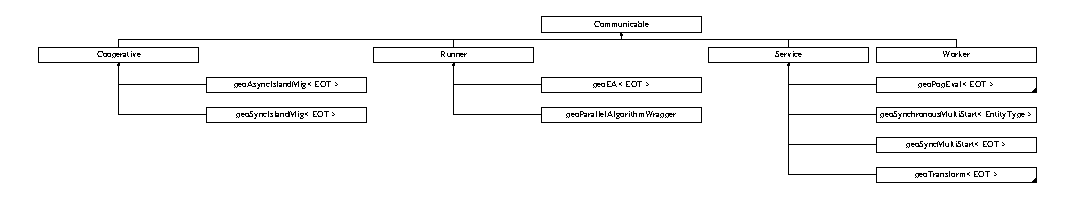
\includegraphics[height=0.843373cm]{classCommunicable}
\end{center}
\end{figure}
\subsection*{Public Member Functions}
\begin{CompactItemize}
\item 
\hypertarget{classCommunicable_8ae1827ecf7569b3db1ed386c7d8ad78}{
\hyperlink{classCommunicable_8ae1827ecf7569b3db1ed386c7d8ad78}{Communicable} ()}
\label{classCommunicable_8ae1827ecf7569b3db1ed386c7d8ad78}

\item 
\hypertarget{classCommunicable_2280b0dfa0d3a515fccf62c2a9fd5f41}{
virtual \hyperlink{classCommunicable_2280b0dfa0d3a515fccf62c2a9fd5f41}{$\sim$Communicable} ()}
\label{classCommunicable_2280b0dfa0d3a515fccf62c2a9fd5f41}

\item 
\hypertarget{classCommunicable_db4307b69b9ccacff55fdbf84b8f50e4}{
COMM\_\-ID \hyperlink{classCommunicable_db4307b69b9ccacff55fdbf84b8f50e4}{get\-Key} ()}
\label{classCommunicable_db4307b69b9ccacff55fdbf84b8f50e4}

\item 
\hypertarget{classCommunicable_e1f8bd1ee810fd73d44315c95998d19d}{
void \hyperlink{classCommunicable_e1f8bd1ee810fd73d44315c95998d19d}{lock} ()}
\label{classCommunicable_e1f8bd1ee810fd73d44315c95998d19d}

\item 
\hypertarget{classCommunicable_caa814847192e71f434fbf9479ede862}{
void \hyperlink{classCommunicable_caa814847192e71f434fbf9479ede862}{unlock} ()}
\label{classCommunicable_caa814847192e71f434fbf9479ede862}

\item 
\hypertarget{classCommunicable_cb53e6534b947bc889aa181d9dbbd13b}{
void \hyperlink{classCommunicable_cb53e6534b947bc889aa181d9dbbd13b}{stop} ()}
\label{classCommunicable_cb53e6534b947bc889aa181d9dbbd13b}

\item 
\hypertarget{classCommunicable_3306a9adb11a0ab5af342c0db9f7bb2a}{
void \hyperlink{classCommunicable_3306a9adb11a0ab5af342c0db9f7bb2a}{resume} ()}
\label{classCommunicable_3306a9adb11a0ab5af342c0db9f7bb2a}

\end{CompactItemize}
\subsection*{Static Public Attributes}
\begin{CompactItemize}
\item 
\hypertarget{classCommunicable_7a6acfdc781a67c9c0ec4f17893f86c3}{
static unsigned \hyperlink{classCommunicable_7a6acfdc781a67c9c0ec4f17893f86c3}{num\_\-comm} = 0}
\label{classCommunicable_7a6acfdc781a67c9c0ec4f17893f86c3}

\end{CompactItemize}
\subsection*{Protected Attributes}
\begin{CompactItemize}
\item 
\hypertarget{classCommunicable_605b0efeffe81326f216c9903f5bbf4c}{
COMM\_\-ID \hyperlink{classCommunicable_605b0efeffe81326f216c9903f5bbf4c}{key}}
\label{classCommunicable_605b0efeffe81326f216c9903f5bbf4c}

\item 
\hypertarget{classCommunicable_cf9639312f71a2f348bc1e7789ccbd9d}{
sem\_\-t \hyperlink{classCommunicable_cf9639312f71a2f348bc1e7789ccbd9d}{sem\_\-lock}}
\label{classCommunicable_cf9639312f71a2f348bc1e7789ccbd9d}

\item 
\hypertarget{classCommunicable_29c53b9191348e0505e3bcba6d8b82b1}{
sem\_\-t \hyperlink{classCommunicable_29c53b9191348e0505e3bcba6d8b82b1}{sem\_\-stop}}
\label{classCommunicable_29c53b9191348e0505e3bcba6d8b82b1}

\end{CompactItemize}


\subsection{Detailed Description}




Definition at line 45 of file communicable.h.

The documentation for this class was generated from the following files:\begin{CompactItemize}
\item 
communicable.h\item 
communicable.cpp\end{CompactItemize}

\hypertarget{classCommunicator}{
\section{Communicator Class Reference}
\label{classCommunicator}\index{Communicator@{Communicator}}
}
Inheritance diagram for Communicator::\begin{figure}[H]
\begin{center}
\leavevmode
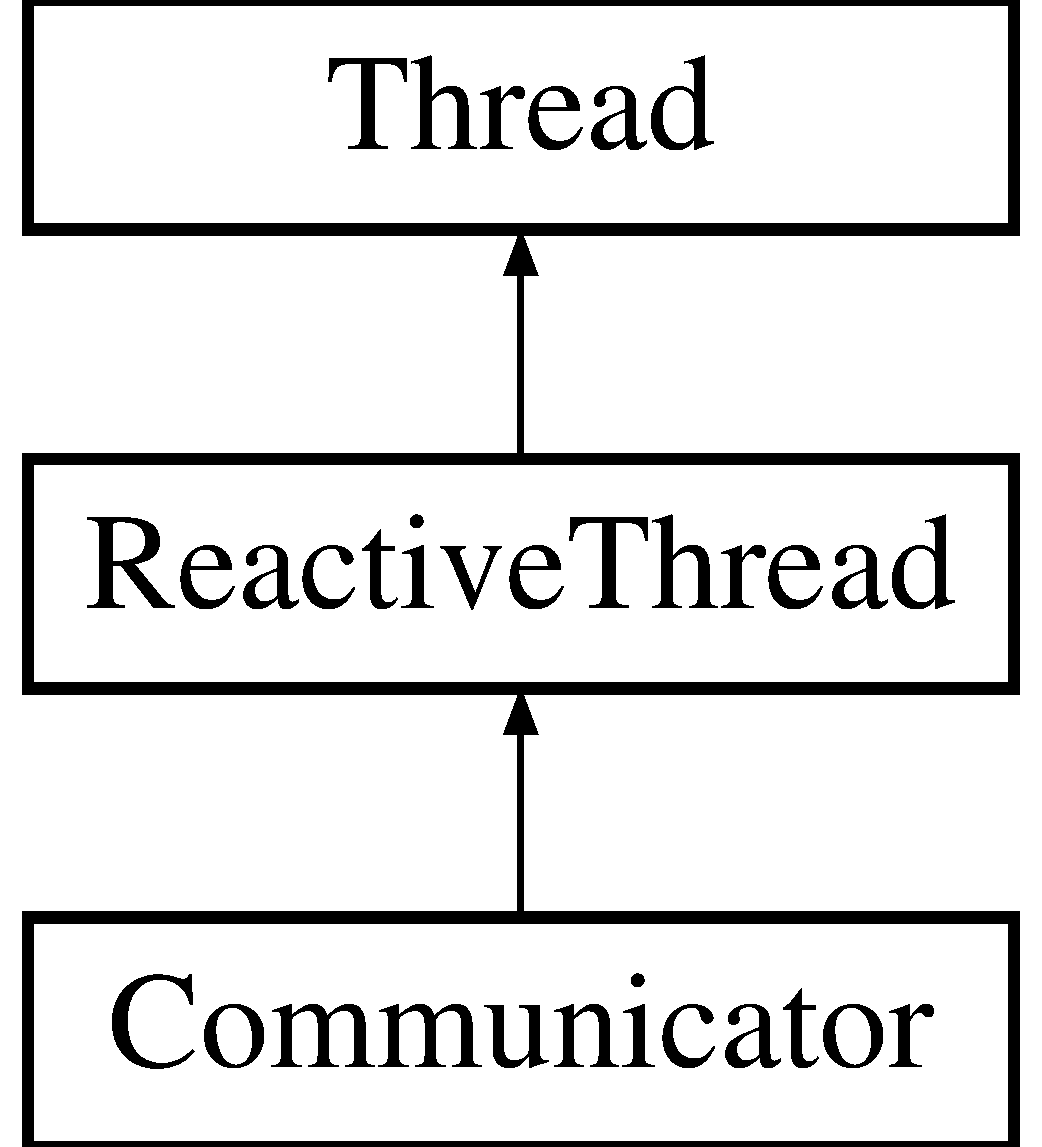
\includegraphics[height=3cm]{classCommunicator}
\end{center}
\end{figure}
\subsection*{Public Member Functions}
\begin{CompactItemize}
\item 
\hypertarget{classCommunicator_7c9dce4ea92bd04d01d53f80c0ef08ee}{
\hyperlink{classCommunicator_7c9dce4ea92bd04d01d53f80c0ef08ee}{Communicator} (int $\ast$\_\-\_\-argc, char $\ast$$\ast$$\ast$\_\-\_\-argv)}
\label{classCommunicator_7c9dce4ea92bd04d01d53f80c0ef08ee}

\item 
\hypertarget{classCommunicator_142fae13b16b166519315f248a513c62}{
void \hyperlink{classCommunicator_142fae13b16b166519315f248a513c62}{start} ()}
\label{classCommunicator_142fae13b16b166519315f248a513c62}

\end{CompactItemize}


\subsection{Detailed Description}




Definition at line 43 of file comm.h.

The documentation for this class was generated from the following files:\begin{CompactItemize}
\item 
comm.h\item 
comm.cpp\end{CompactItemize}

\hypertarget{classCooperative}{
\section{Cooperative Class Reference}
\label{classCooperative}\index{Cooperative@{Cooperative}}
}
Inheritance diagram for Cooperative::\begin{figure}[H]
\begin{center}
\leavevmode
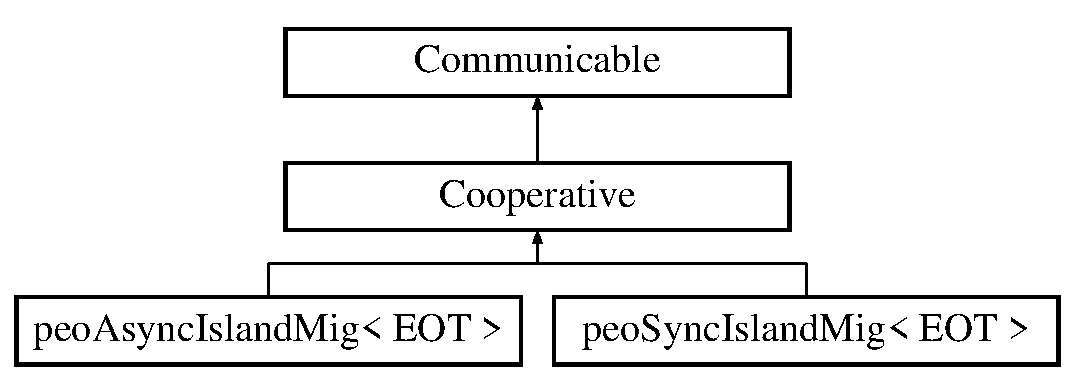
\includegraphics[height=3cm]{classCooperative}
\end{center}
\end{figure}
\subsection*{Public Member Functions}
\begin{CompactItemize}
\item 
\hypertarget{classCooperative_4012b4e8329e87d26ee266491e1a883e}{
\hyperlink{classRunner}{Runner} $\ast$ \hyperlink{classCooperative_4012b4e8329e87d26ee266491e1a883e}{get\-Owner} ()}
\label{classCooperative_4012b4e8329e87d26ee266491e1a883e}

\item 
\hypertarget{classCooperative_fe7b022567174c8305bc78d8c5749b12}{
void \hyperlink{classCooperative_fe7b022567174c8305bc78d8c5749b12}{set\-Owner} (\hyperlink{classRunner}{Runner} \&\_\-\_\-runner)}
\label{classCooperative_fe7b022567174c8305bc78d8c5749b12}

\item 
\hypertarget{classCooperative_c609f2a1200da7d1ac96005602515fc6}{
void \hyperlink{classCooperative_c609f2a1200da7d1ac96005602515fc6}{send} (\hyperlink{classCooperative}{Cooperative} $\ast$\_\-\_\-coop)}
\label{classCooperative_c609f2a1200da7d1ac96005602515fc6}

\item 
\hypertarget{classCooperative_4439ddeaa1246a2e44c003bfb781739b}{
virtual void \hyperlink{classCooperative_4439ddeaa1246a2e44c003bfb781739b}{notify\-Sending} ()}
\label{classCooperative_4439ddeaa1246a2e44c003bfb781739b}

\end{CompactItemize}
\subsection*{Private Attributes}
\begin{CompactItemize}
\item 
\hypertarget{classCooperative_7604f094479d08154ede4996a45bf79e}{
\hyperlink{classRunner}{Runner} $\ast$ \hyperlink{classCooperative_7604f094479d08154ede4996a45bf79e}{owner}}
\label{classCooperative_7604f094479d08154ede4996a45bf79e}

\end{CompactItemize}


\subsection{Detailed Description}




Definition at line 45 of file cooperative.h.

The documentation for this class was generated from the following files:\begin{CompactItemize}
\item 
cooperative.h\item 
coop.cpp\end{CompactItemize}

\hypertarget{classDisplayBestRoute}{
\section{Display\-Best\-Route Class Reference}
\label{classDisplayBestRoute}\index{DisplayBestRoute@{DisplayBestRoute}}
}
Inheritance diagram for Display\-Best\-Route::\begin{figure}[H]
\begin{center}
\leavevmode
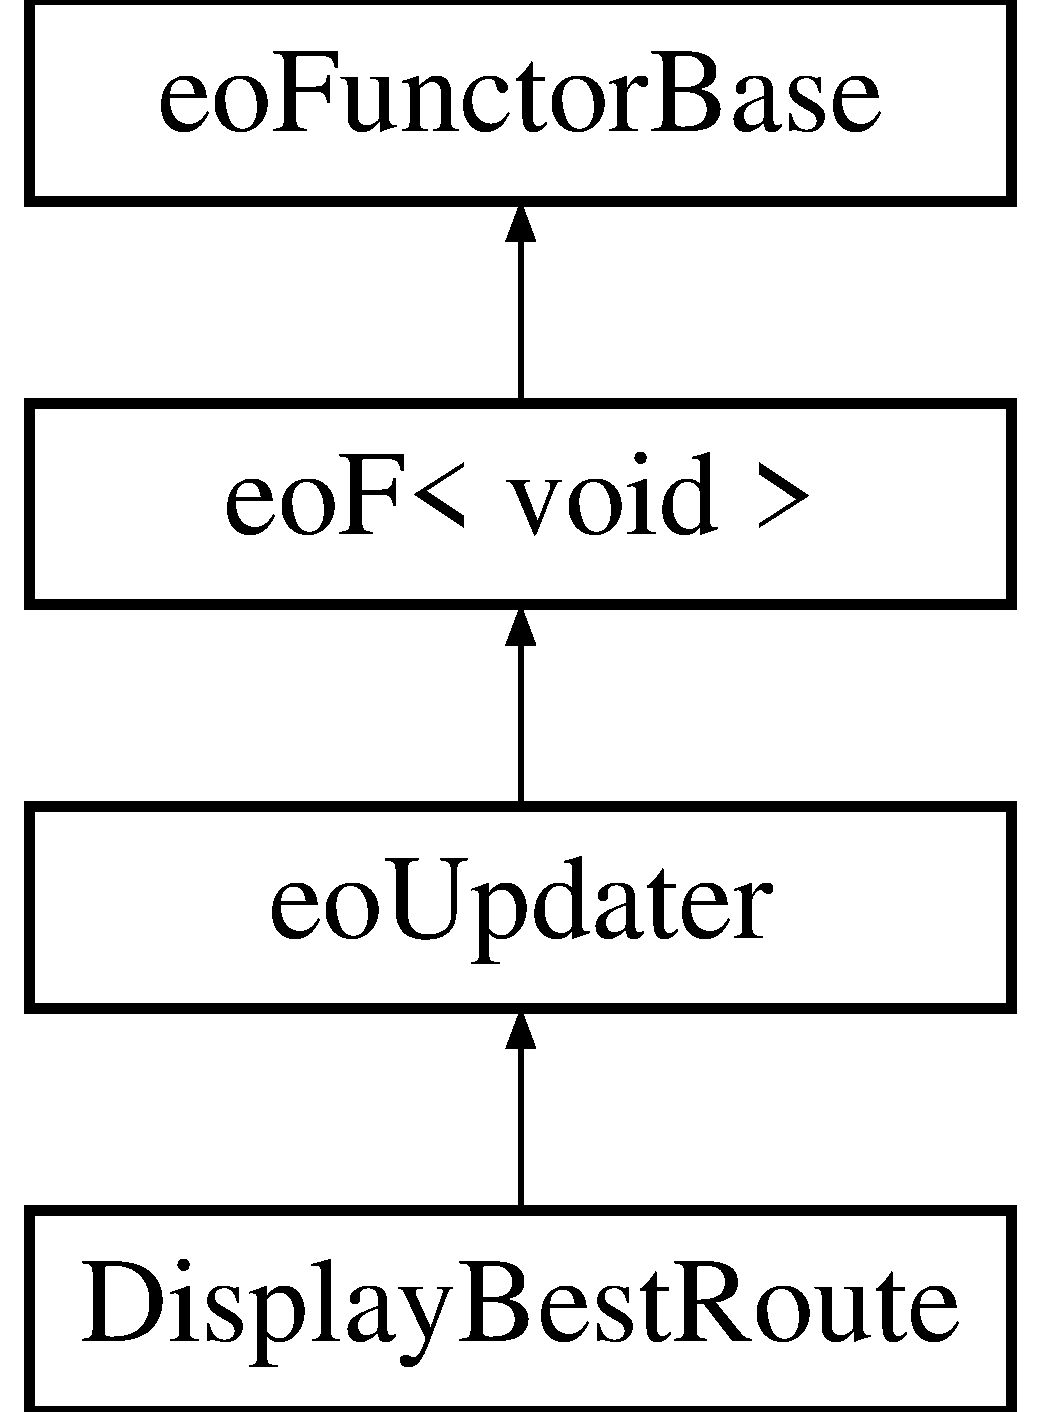
\includegraphics[height=4cm]{classDisplayBestRoute}
\end{center}
\end{figure}
\subsection*{Public Member Functions}
\begin{CompactItemize}
\item 
\hypertarget{classDisplayBestRoute_db263e38f1e82174f811bf62f323f87f}{
\hyperlink{classDisplayBestRoute_db263e38f1e82174f811bf62f323f87f}{Display\-Best\-Route} (\bf{eo\-Pop}$<$ \bf{Route} $>$ \&\_\-\_\-pop)}
\label{classDisplayBestRoute_db263e38f1e82174f811bf62f323f87f}

\item 
\hypertarget{classDisplayBestRoute_ee879344a6d8b81a04d4eabbed2c7a04}{
void \hyperlink{classDisplayBestRoute_ee879344a6d8b81a04d4eabbed2c7a04}{operator()} ()}
\label{classDisplayBestRoute_ee879344a6d8b81a04d4eabbed2c7a04}

\end{CompactItemize}
\subsection*{Private Attributes}
\begin{CompactItemize}
\item 
\hypertarget{classDisplayBestRoute_5270aabbf294d2deca9878934216eb89}{
\bf{eo\-Pop}$<$ \bf{Route} $>$ \& \hyperlink{classDisplayBestRoute_5270aabbf294d2deca9878934216eb89}{pop}}
\label{classDisplayBestRoute_5270aabbf294d2deca9878934216eb89}

\end{CompactItemize}


\subsection{Detailed Description}




Definition at line 46 of file display\_\-best\_\-route.h.

The documentation for this class was generated from the following files:\begin{CompactItemize}
\item 
display\_\-best\_\-route.h\item 
display\_\-best\_\-route.cpp\end{CompactItemize}

\hypertarget{classMergeRouteEval}{
\section{Merge\-Route\-Eval Class Reference}
\label{classMergeRouteEval}\index{MergeRouteEval@{MergeRouteEval}}
}
Inheritance diagram for Merge\-Route\-Eval::\begin{figure}[H]
\begin{center}
\leavevmode
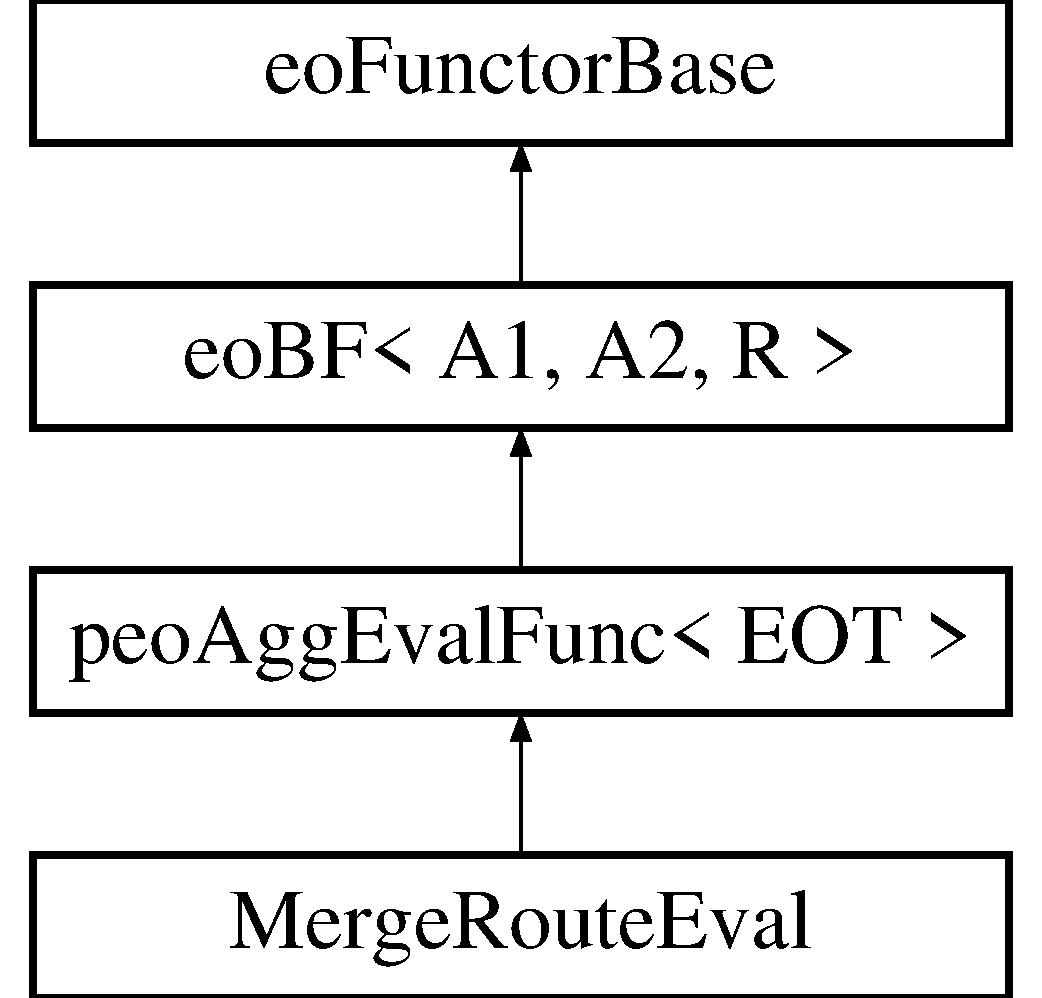
\includegraphics[height=2cm]{classMergeRouteEval}
\end{center}
\end{figure}
\subsection*{Public Member Functions}
\begin{CompactItemize}
\item 
\hypertarget{classMergeRouteEval_29cb0028ac0df4b2cee3a809c8f35dea}{
void \hyperlink{classMergeRouteEval_29cb0028ac0df4b2cee3a809c8f35dea}{operator()} (Route \&\_\-\_\-route, const int \&\_\-\_\-part\_\-fit)}
\label{classMergeRouteEval_29cb0028ac0df4b2cee3a809c8f35dea}

\end{CompactItemize}


\subsection{Detailed Description}




Definition at line 44 of file merge\_\-route\_\-eval.h.

The documentation for this class was generated from the following files:\begin{CompactItemize}
\item 
merge\_\-route\_\-eval.h\item 
merge\_\-route\_\-eval.cpp\end{CompactItemize}

\hypertarget{classpeoAggEvalFunc}{
\section{peo\-Agg\-Eval\-Func$<$ EOT $>$ Class Template Reference}
\label{classpeoAggEvalFunc}\index{peoAggEvalFunc@{peoAggEvalFunc}}
}
The \hyperlink{classpeoAggEvalFunc}{peo\-Agg\-Eval\-Func} class offers only the interface for creating aggregate evaluation functions - there are no direct internal functions provided.  


{\tt \#include $<$peo\-Agg\-Eval\-Func.h$>$}

Inheritance diagram for peo\-Agg\-Eval\-Func$<$ EOT $>$::\begin{figure}[H]
\begin{center}
\leavevmode
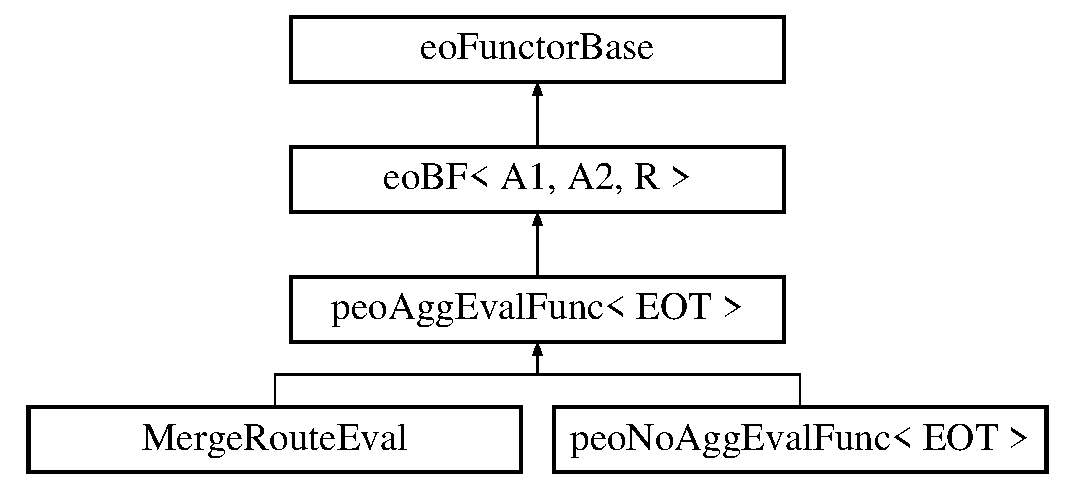
\includegraphics[height=4cm]{classpeoAggEvalFunc}
\end{center}
\end{figure}


\subsection{Detailed Description}
\subsubsection*{template$<$class EOT$>$ class peo\-Agg\-Eval\-Func$<$ EOT $>$}

The \hyperlink{classpeoAggEvalFunc}{peo\-Agg\-Eval\-Func} class offers only the interface for creating aggregate evaluation functions - there are no direct internal functions provided. 

The class inherits {\bf public eo\-BF$<$ EOT\&, const typename EOT :: Fitness\&, void $>$} thus requiring, for the derived classes, the creation of a function having the following signature:

\begin{TabularC}{2}
\hline
void operator()( EOT\& \_\-\_\-eot, const typename EOT :: Fitness\& \_\-\_\-partial\_\-fittness ); ~ &~  \\\hline
\end{TabularC}


The aggregation object is called in an iterative manner for each of the results obtained by applying partial evaluation functions. 



Definition at line 53 of file peo\-Agg\-Eval\-Func.h.

The documentation for this class was generated from the following file:\begin{CompactItemize}
\item 
peo\-Agg\-Eval\-Func.h\end{CompactItemize}

\hypertarget{classpeoAsyncIslandMig}{
\section{peo\-Async\-Island\-Mig$<$ TYPESELECT, TYPEREPLACE $>$ Class Template Reference}
\label{classpeoAsyncIslandMig}\index{peoAsyncIslandMig@{peoAsyncIslandMig}}
}
Specific class for a asynchronous migration.  


{\tt \#include $<$peo\-Async\-Island\-Mig.h$>$}

Inheritance diagram for peo\-Async\-Island\-Mig$<$ TYPESELECT, TYPEREPLACE $>$::\begin{figure}[H]
\begin{center}
\leavevmode
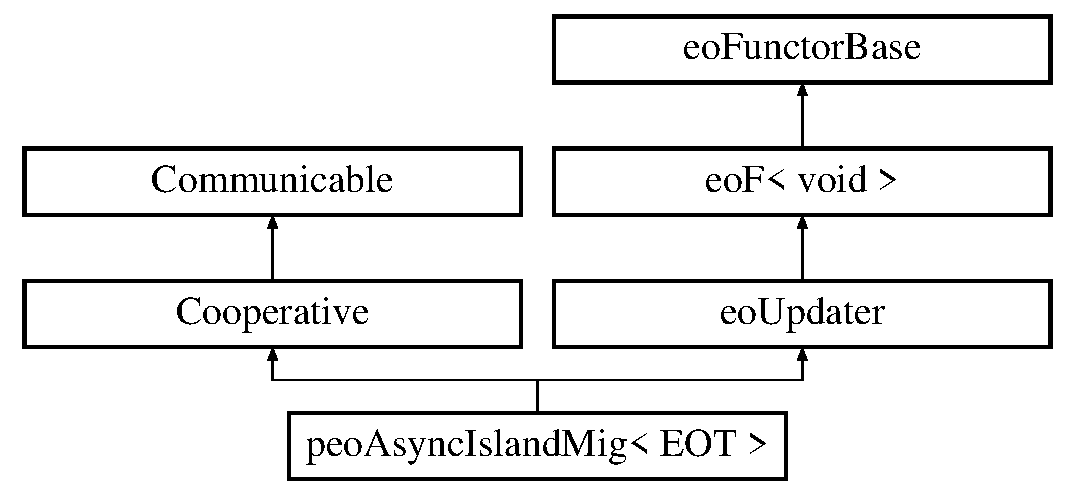
\includegraphics[height=3cm]{classpeoAsyncIslandMig}
\end{center}
\end{figure}
\subsection*{Public Member Functions}
\begin{CompactItemize}
\item 
\hyperlink{classpeoAsyncIslandMig_e40ddd54734b018ab4e5c3f2bbd5a49c}{peo\-Async\-Island\-Mig} (\hyperlink{classcontinuator}{continuator} \&\_\-\_\-cont, \hyperlink{classselector}{selector}$<$ TYPESELECT $>$ \&\_\-\_\-select, \hyperlink{classreplacement}{replacement}$<$ TYPEREPLACE $>$ \&\_\-\_\-replace, \hyperlink{classTopology}{Topology} \&\_\-\_\-topology)
\item 
\hypertarget{classpeoAsyncIslandMig_d56e189f269dde8d68a4b007f05edaff}{
void \hyperlink{classpeoAsyncIslandMig_d56e189f269dde8d68a4b007f05edaff}{operator()} ()}
\label{classpeoAsyncIslandMig_d56e189f269dde8d68a4b007f05edaff}

\begin{CompactList}\small\item\em operator \item\end{CompactList}\item 
\hypertarget{classpeoAsyncIslandMig_0f5f1700920f9ced71ef63b0576e3f14}{
void \hyperlink{classpeoAsyncIslandMig_0f5f1700920f9ced71ef63b0576e3f14}{pack} ()}
\label{classpeoAsyncIslandMig_0f5f1700920f9ced71ef63b0576e3f14}

\begin{CompactList}\small\item\em Function realizing packages. \item\end{CompactList}\item 
\hypertarget{classpeoAsyncIslandMig_c32a27e387bcd8ce383a4cb1732dbed8}{
void \hyperlink{classpeoAsyncIslandMig_c32a27e387bcd8ce383a4cb1732dbed8}{unpack} ()}
\label{classpeoAsyncIslandMig_c32a27e387bcd8ce383a4cb1732dbed8}

\begin{CompactList}\small\item\em Function reconstituting packages. \item\end{CompactList}\item 
\hypertarget{classpeoAsyncIslandMig_0a0524a90d0b31bc4c8bfa4f39708b0f}{
void \hyperlink{classpeoAsyncIslandMig_0a0524a90d0b31bc4c8bfa4f39708b0f}{pack\-Synchronize\-Req} ()}
\label{classpeoAsyncIslandMig_0a0524a90d0b31bc4c8bfa4f39708b0f}

\begin{CompactList}\small\item\em Function pack\-Synchronize\-Req. \item\end{CompactList}\end{CompactItemize}
\subsection*{Private Member Functions}
\begin{CompactItemize}
\item 
\hypertarget{classpeoAsyncIslandMig_2470f8ee04bc762c010c7ebb2392831d}{
void \hyperlink{classpeoAsyncIslandMig_2470f8ee04bc762c010c7ebb2392831d}{emigrate} ()}
\label{classpeoAsyncIslandMig_2470f8ee04bc762c010c7ebb2392831d}

\begin{CompactList}\small\item\em Function which sends some emigrants. \item\end{CompactList}\item 
\hypertarget{classpeoAsyncIslandMig_75a6592d63879773b39c9594b94fb942}{
void \hyperlink{classpeoAsyncIslandMig_75a6592d63879773b39c9594b94fb942}{immigrate} ()}
\label{classpeoAsyncIslandMig_75a6592d63879773b39c9594b94fb942}

\begin{CompactList}\small\item\em Function which receives some immigrants. \item\end{CompactList}\end{CompactItemize}
\subsection*{Private Attributes}
\begin{CompactItemize}
\item 
\hyperlink{classcontinuator}{continuator} \& \hyperlink{classpeoAsyncIslandMig_b7a4049f66f99f9e7ec5c785042ee06a}{cont}
\item 
\hypertarget{classpeoAsyncIslandMig_57d9ed6da844aa67a8a3328dfbbd03e0}{
\hyperlink{classselector}{selector}$<$ TYPESELECT $>$ \& \hyperlink{classpeoAsyncIslandMig_57d9ed6da844aa67a8a3328dfbbd03e0}{select}}
\label{classpeoAsyncIslandMig_57d9ed6da844aa67a8a3328dfbbd03e0}

\item 
\hypertarget{classpeoAsyncIslandMig_2013056fed65e4f0bb55a7334c261c50}{
\hyperlink{classreplacement}{replacement}$<$ TYPEREPLACE $>$ \& \hyperlink{classpeoAsyncIslandMig_2013056fed65e4f0bb55a7334c261c50}{replace}}
\label{classpeoAsyncIslandMig_2013056fed65e4f0bb55a7334c261c50}

\item 
\hypertarget{classpeoAsyncIslandMig_e70e843ec1fc9e2fc6a124588fbc08d5}{
\hyperlink{classTopology}{Topology} \& \hyperlink{classpeoAsyncIslandMig_e70e843ec1fc9e2fc6a124588fbc08d5}{topology}}
\label{classpeoAsyncIslandMig_e70e843ec1fc9e2fc6a124588fbc08d5}

\item 
\hypertarget{classpeoAsyncIslandMig_3fa5d4df0bdd4a3c58a9f1bd38d628f9}{
std::queue$<$ TYPEREPLACE $>$ \hyperlink{classpeoAsyncIslandMig_3fa5d4df0bdd4a3c58a9f1bd38d628f9}{imm}}
\label{classpeoAsyncIslandMig_3fa5d4df0bdd4a3c58a9f1bd38d628f9}

\item 
\hypertarget{classpeoAsyncIslandMig_04c6a5767efe3e4deb914a6a8ceb3fd2}{
std::queue$<$ TYPESELECT $>$ \hyperlink{classpeoAsyncIslandMig_04c6a5767efe3e4deb914a6a8ceb3fd2}{em}}
\label{classpeoAsyncIslandMig_04c6a5767efe3e4deb914a6a8ceb3fd2}

\item 
\hypertarget{classpeoAsyncIslandMig_9ead40772ef2fabea02fe93d1814f0a5}{
std::queue$<$ \hyperlink{classCooperative}{Cooperative} $\ast$ $>$ \hyperlink{classpeoAsyncIslandMig_9ead40772ef2fabea02fe93d1814f0a5}{coop\_\-em}}
\label{classpeoAsyncIslandMig_9ead40772ef2fabea02fe93d1814f0a5}

\end{CompactItemize}


\subsection{Detailed Description}
\subsubsection*{template$<$class TYPESELECT, class TYPEREPLACE$>$ class peo\-Async\-Island\-Mig$<$ TYPESELECT, TYPEREPLACE $>$}

Specific class for a asynchronous migration. 

\begin{Desc}
\item[See also:]\hyperlink{classCooperative}{Cooperative} eo\-Updater \end{Desc}
\begin{Desc}
\item[Version:]2.0 \end{Desc}
\begin{Desc}
\item[Date:]january 2008 \end{Desc}




Definition at line 64 of file peo\-Async\-Island\-Mig.h.

\subsection{Constructor \& Destructor Documentation}
\hypertarget{classpeoAsyncIslandMig_e40ddd54734b018ab4e5c3f2bbd5a49c}{
\index{peoAsyncIslandMig@{peo\-Async\-Island\-Mig}!peoAsyncIslandMig@{peoAsyncIslandMig}}
\index{peoAsyncIslandMig@{peoAsyncIslandMig}!peoAsyncIslandMig@{peo\-Async\-Island\-Mig}}
\subsubsection[peoAsyncIslandMig]{\setlength{\rightskip}{0pt plus 5cm}template$<$class TYPESELECT, class TYPEREPLACE$>$ \hyperlink{classpeoAsyncIslandMig}{peo\-Async\-Island\-Mig}$<$ TYPESELECT, TYPEREPLACE $>$::\hyperlink{classpeoAsyncIslandMig}{peo\-Async\-Island\-Mig} (\hyperlink{classcontinuator}{continuator} \& {\em \_\-\_\-cont}, \hyperlink{classselector}{selector}$<$ TYPESELECT $>$ \& {\em \_\-\_\-select}, \hyperlink{classreplacement}{replacement}$<$ TYPEREPLACE $>$ \& {\em \_\-\_\-replace}, \hyperlink{classTopology}{Topology} \& {\em \_\-\_\-topology})}}
\label{classpeoAsyncIslandMig_e40ddd54734b018ab4e5c3f2bbd5a49c}


\begin{Desc}
\item[Parameters:]
\begin{description}
\item[{\em continuator}]\& \_\-\_\-cont \item[{\em selector}]$<$TYPE$>$ \& \_\-\_\-select \item[{\em replacement}]$<$TYPE$>$ \& \_\-\_\-replace \item[{\em Topology\&}]\_\-\_\-topology \end{description}
\end{Desc}


Definition at line 114 of file peo\-Async\-Island\-Mig.h.

References Topology::add().

\subsection{Member Data Documentation}
\hypertarget{classpeoAsyncIslandMig_b7a4049f66f99f9e7ec5c785042ee06a}{
\index{peoAsyncIslandMig@{peo\-Async\-Island\-Mig}!cont@{cont}}
\index{cont@{cont}!peoAsyncIslandMig@{peo\-Async\-Island\-Mig}}
\subsubsection[cont]{\setlength{\rightskip}{0pt plus 5cm}template$<$class TYPESELECT, class TYPEREPLACE$>$ \hyperlink{classcontinuator}{continuator}\& \hyperlink{classpeoAsyncIslandMig}{peo\-Async\-Island\-Mig}$<$ TYPESELECT, TYPEREPLACE $>$::\hyperlink{classpeoAsyncIslandMig_b7a4049f66f99f9e7ec5c785042ee06a}{cont}\hspace{0.3cm}{\tt  \mbox{[}private\mbox{]}}}}
\label{classpeoAsyncIslandMig_b7a4049f66f99f9e7ec5c785042ee06a}


\begin{Desc}
\item[Parameters:]
\begin{description}
\item[{\em continuator}]\& cont \item[{\em selector}]$<$TYPESELECT$>$ \& select \item[{\em replacement}]$<$TYPEREPLACE$>$ \& replace \item[{\em Topology\&}]topology \item[{\em std}]:: queue$<$ TYPEREPLACE $>$ imm \item[{\em std}]:: queue$<$ TYPESELECT $>$ em \item[{\em std}]:: queue$<$ Cooperative$\ast$ $>$ coop\_\-em \end{description}
\end{Desc}


Definition at line 104 of file peo\-Async\-Island\-Mig.h.

Referenced by peo\-Async\-Island\-Mig$<$ TYPESELECT, TYPEREPLACE $>$::operator()().

The documentation for this class was generated from the following file:\begin{CompactItemize}
\item 
peo\-Async\-Island\-Mig.h\end{CompactItemize}

\hypertarget{classpeoEA}{
\section{peo\-EA$<$ EOT $>$ Class Template Reference}
\label{classpeoEA}\index{peoEA@{peoEA}}
}
The \hyperlink{classpeoEA}{peo\-EA} class offers an elementary evolutionary algorithm implementation.  


{\tt \#include $<$peo\-EA.h$>$}

Inheritance diagram for peo\-EA$<$ EOT $>$::\begin{figure}[H]
\begin{center}
\leavevmode
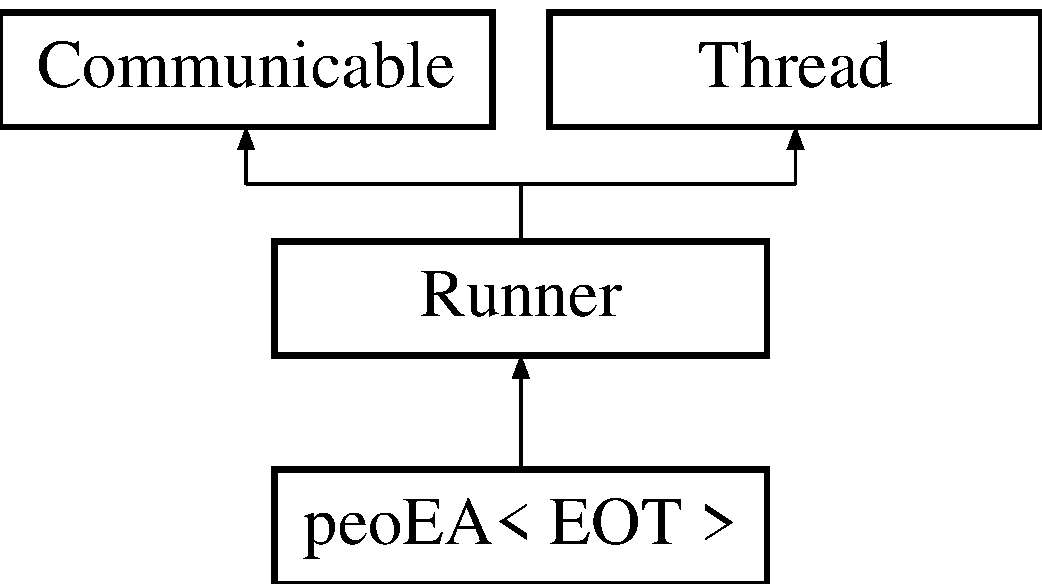
\includegraphics[height=3cm]{classpeoEA}
\end{center}
\end{figure}
\subsection*{Public Member Functions}
\begin{CompactItemize}
\item 
\hyperlink{classpeoEA_dbfc4f8907bef234602149229f132371}{peo\-EA} (\bf{eo\-Continue}$<$ EOT $>$ \&\_\-\_\-cont, \hyperlink{classpeoPopEval}{peo\-Pop\-Eval}$<$ EOT $>$ \&\_\-\_\-pop\_\-eval, \bf{eo\-Select}$<$ EOT $>$ \&\_\-\_\-select, \hyperlink{classpeoTransform}{peo\-Transform}$<$ EOT $>$ \&\_\-\_\-trans, \bf{eo\-Replacement}$<$ EOT $>$ \&\_\-\_\-replace)
\begin{CompactList}\small\item\em Constructor for the evolutionary algorithm object - several basic parameters have to be specified, allowing for different levels of parallelism. \item\end{CompactList}\item 
\hypertarget{classpeoEA_6ab8c321d29350634143a2a01cf2ad24}{
void \hyperlink{classpeoEA_6ab8c321d29350634143a2a01cf2ad24}{run} ()}
\label{classpeoEA_6ab8c321d29350634143a2a01cf2ad24}

\begin{CompactList}\small\item\em Evolutionary algorithm function - a side effect of the fact that the class is derived from the {\bf \hyperlink{classRunner}{Runner}} class, thus requiring the existence of a {\em run\/} function, the algorithm being executed on a distinct thread. \item\end{CompactList}\item 
void \hyperlink{classpeoEA_3c709e3b2491147d26fee36138644613}{operator()} (\bf{eo\-Pop}$<$ EOT $>$ \&\_\-\_\-pop)
\begin{CompactList}\small\item\em \doxyref{Function} operator for specifying the population to be associated with the algorithm. \item\end{CompactList}\end{CompactItemize}
\subsection*{Private Attributes}
\begin{CompactItemize}
\item 
\hypertarget{classpeoEA_5f015eebf42f176b9fe322488c446c2a}{
\bf{eo\-Continue}$<$ EOT $>$ \& \hyperlink{classpeoEA_5f015eebf42f176b9fe322488c446c2a}{cont}}
\label{classpeoEA_5f015eebf42f176b9fe322488c446c2a}

\item 
\hypertarget{classpeoEA_9140259f50c9186edcb062b023624c96}{
\hyperlink{classpeoPopEval}{peo\-Pop\-Eval}$<$ EOT $>$ \& \hyperlink{classpeoEA_9140259f50c9186edcb062b023624c96}{pop\_\-eval}}
\label{classpeoEA_9140259f50c9186edcb062b023624c96}

\item 
\hypertarget{classpeoEA_2d8428d69fdd6aefefbaf543fdd46d19}{
\bf{eo\-Select}$<$ EOT $>$ \& \hyperlink{classpeoEA_2d8428d69fdd6aefefbaf543fdd46d19}{select}}
\label{classpeoEA_2d8428d69fdd6aefefbaf543fdd46d19}

\item 
\hypertarget{classpeoEA_713c77935eb8aafebfb9488cfaa4a363}{
\hyperlink{classpeoTransform}{peo\-Transform}$<$ EOT $>$ \& \hyperlink{classpeoEA_713c77935eb8aafebfb9488cfaa4a363}{trans}}
\label{classpeoEA_713c77935eb8aafebfb9488cfaa4a363}

\item 
\hypertarget{classpeoEA_9bd2d4356cf7e69e3141dc269213aa8a}{
\bf{eo\-Replacement}$<$ EOT $>$ \& \hyperlink{classpeoEA_9bd2d4356cf7e69e3141dc269213aa8a}{replace}}
\label{classpeoEA_9bd2d4356cf7e69e3141dc269213aa8a}

\item 
\hypertarget{classpeoEA_c0b110e410bc16283e8339f24b733772}{
\bf{eo\-Pop}$<$ EOT $>$ $\ast$ \hyperlink{classpeoEA_c0b110e410bc16283e8339f24b733772}{pop}}
\label{classpeoEA_c0b110e410bc16283e8339f24b733772}

\end{CompactItemize}


\subsection{Detailed Description}
\subsubsection*{template$<$class EOT$>$ class peo\-EA$<$ EOT $>$}

The \hyperlink{classpeoEA}{peo\-EA} class offers an elementary evolutionary algorithm implementation. 

In addition, as compared with the algorithms provided by the \doxyref{EO} framework, the \hyperlink{classpeoEA}{peo\-EA} class has the underlying necessary structure for including, for example, parallel evaluation and parallel transformation operators, migration operators etc. Although there is no restriction on using the algorithms provided by the \doxyref{EO} framework, the drawback resides in the fact that the \doxyref{EO} implementation is exclusively sequential and, in consequence, no parallelism is provided. A simple example for constructing a \hyperlink{classpeoEA}{peo\-EA} object:

\begin{TabularC}{2}
\hline
... ~ &~  \\\hline
eo\-Pop$<$ EOT $>$ population( POP\_\-SIZE, pop\-Initializer ); ~ &// creation of a population with POP\_\-SIZE individuals - the pop\-Initializer is a functor to be called for each individual \\\hline
~  &~  \\\hline
eo\-Gen\-Continue$<$ EOT $>$ ea\-Cont( NUM\_\-GEN ); ~ &// number of generations for the evolutionary algorithm \\\hline
eo\-Check\-Point$<$ EOT $>$ ea\-Checkpoint\-Continue( ea\-Cont ); ~ &// checkpoint incorporating the continuation criterion - startpoint for adding other checkpoint objects \\\hline
~  &~  \\\hline
peo\-Seq\-Pop\-Eval$<$ EOT $>$ ea\-Pop\-Eval( eval\-Function ); ~ &// sequential evaluation functor wrapper - eval\-Function represents the actual evaluation functor  \\\hline
~  &~  \\\hline
eo\-Ranking\-Select$<$ EOT $>$ selection\-Strategy; ~ &// selection strategy for creating the offspring population - a simple ranking selection in this case  \\\hline
eo\-Select\-Number$<$ EOT $>$ ea\-Select( selection\-Strategy, POP\_\-SIZE ); ~ &// the number of individuals to be selected for creating the offspring population  \\\hline
eo\-Ranking\-Select$<$ EOT $>$ selection\-Strategy; ~ &// selection strategy for creating the offspring population - a simple ranking selection in this case  \\\hline
~  &~  \\\hline
eo\-SGATransform$<$ EOT $>$ transform( crossover, CROSS\_\-RATE, mutation, MUT\_\-RATE ); ~ &// transformation operator - crossover and mutation operators with their associated probabilities  \\\hline
peo\-Seq\-Transform$<$ EOT $>$ ea\-Transform( transform ); ~ &// Paradis\-EO specific sequential operator - a parallel version may be specified in the same manner  \\\hline
~  &~  \\\hline
eo\-Plus\-Replacement$<$ EOT $>$ ea\-Replace; ~ &// replacement strategy - for integrating the offspring resulting individuals in the initial population  \\\hline
~  &~  \\\hline
peo\-EA$<$ EOT $>$ ea\-Alg( ea\-Checkpoint\-Continue, ea\-Pop\-Eval, ea\-Select, ea\-Transform, ea\-Replace ); ~ &// Paradis\-EO evolutionary algorithm integrating the above defined objects  \\\hline
ea\-Alg( population ); ~ &// specifying the initial population for the algorithm  \\\hline
... ~ &~  \\\hline
\end{TabularC}




Definition at line 82 of file peo\-EA.h.

\subsection{Constructor \& Destructor Documentation}
\hypertarget{classpeoEA_dbfc4f8907bef234602149229f132371}{
\index{peoEA@{peo\-EA}!peoEA@{peoEA}}
\index{peoEA@{peoEA}!peoEA@{peo\-EA}}
\subsubsection[peoEA]{\setlength{\rightskip}{0pt plus 5cm}template$<$class EOT$>$ \hyperlink{classpeoEA}{peo\-EA}$<$ EOT $>$::\hyperlink{classpeoEA}{peo\-EA} (\bf{eo\-Continue}$<$ EOT $>$ \& {\em \_\-\_\-cont}, \hyperlink{classpeoPopEval}{peo\-Pop\-Eval}$<$ EOT $>$ \& {\em \_\-\_\-pop\_\-eval}, \bf{eo\-Select}$<$ EOT $>$ \& {\em \_\-\_\-select}, \hyperlink{classpeoTransform}{peo\-Transform}$<$ EOT $>$ \& {\em \_\-\_\-trans}, \bf{eo\-Replacement}$<$ EOT $>$ \& {\em \_\-\_\-replace})}}
\label{classpeoEA_dbfc4f8907bef234602149229f132371}


Constructor for the evolutionary algorithm object - several basic parameters have to be specified, allowing for different levels of parallelism. 

Depending on the requirements, a sequential or a parallel evaluation operator may be specified or, in the same manner, a sequential or a parallel transformation operator may be given as parameter. Out of the box objects may be provided, from the \doxyref{EO} package, for example, or custom defined ones may be specified, provided that they are derived from the correct base classes.

\begin{Desc}
\item[Parameters:]
\begin{description}
\item[{\em eo\-Continue$<$}]EOT $>$\& \_\-\_\-cont - continuation criterion specifying whether the algorithm should continue or not; \item[{\em peo\-Pop\-Eval$<$}]EOT $>$\& \_\-\_\-pop\_\-eval - evaluation operator; it allows the specification of parallel evaluation operators, aggregate evaluation functions, etc.; \item[{\em eo\-Select$<$}]EOT $>$\& \_\-\_\-select - selection strategy to be applied for constructing a list of offspring individuals; \item[{\em peo\-Transform$<$}]EOT $>$\& \_\-\_\-trans - transformation operator, i.e. crossover and mutation; allows for sequential or parallel transform; \item[{\em eo\-Replacement$<$}]EOT $>$\& \_\-\_\-replace - replacement strategy for integrating the offspring individuals in the initial population; \end{description}
\end{Desc}


Definition at line 126 of file peo\-EA.h.

References peo\-EA$<$ EOT $>$::pop\_\-eval, and peo\-EA$<$ EOT $>$::trans.

\subsection{Member Function Documentation}
\hypertarget{classpeoEA_3c709e3b2491147d26fee36138644613}{
\index{peoEA@{peo\-EA}!operator()@{operator()}}
\index{operator()@{operator()}!peoEA@{peo\-EA}}
\subsubsection[operator()]{\setlength{\rightskip}{0pt plus 5cm}template$<$class EOT$>$ void \hyperlink{classpeoEA}{peo\-EA}$<$ EOT $>$::operator() (\bf{eo\-Pop}$<$ EOT $>$ \& {\em \_\-\_\-pop})}}
\label{classpeoEA_3c709e3b2491147d26fee36138644613}


\doxyref{Function} operator for specifying the population to be associated with the algorithm. 

\begin{Desc}
\item[Parameters:]
\begin{description}
\item[{\em eo\-Pop$<$}]EOT $>$\& \_\-\_\-pop - initial population of the algorithm, to be iteratively evolved; \end{description}
\end{Desc}


Definition at line 142 of file peo\-EA.h.

References peo\-EA$<$ EOT $>$::pop.

The documentation for this class was generated from the following file:\begin{CompactItemize}
\item 
peo\-EA.h\end{CompactItemize}

\hypertarget{classpeoNoAggEvalFunc}{
\section{peo\-No\-Agg\-Eval\-Func$<$ EOT $>$ Class Template Reference}
\label{classpeoNoAggEvalFunc}\index{peoNoAggEvalFunc@{peoNoAggEvalFunc}}
}
The \hyperlink{classpeoNoAggEvalFunc}{peo\-No\-Agg\-Eval\-Func} class does nothing more than an association between a fitness value and a specified individual.  


{\tt \#include $<$peo\-No\-Agg\-Eval\-Func.h$>$}

Inheritance diagram for peo\-No\-Agg\-Eval\-Func$<$ EOT $>$::\begin{figure}[H]
\begin{center}
\leavevmode
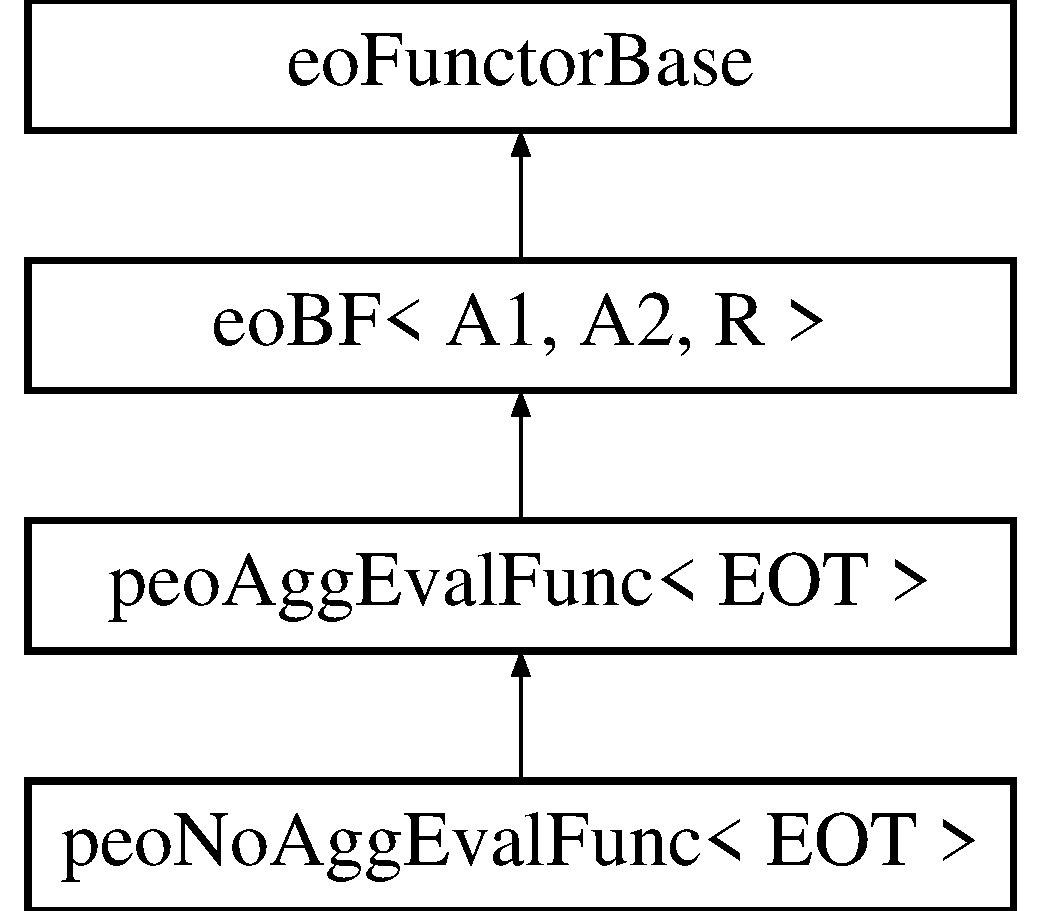
\includegraphics[height=4cm]{classpeoNoAggEvalFunc}
\end{center}
\end{figure}
\subsection*{Public Member Functions}
\begin{CompactItemize}
\item 
\hypertarget{classpeoNoAggEvalFunc_1a69ee1af8745ac75c864bf884436de5}{
void \hyperlink{classpeoNoAggEvalFunc_1a69ee1af8745ac75c864bf884436de5}{operator()} (EOT \&\_\-\_\-sol, const typename EOT::Fitness \&\_\-\_\-fit)}
\label{classpeoNoAggEvalFunc_1a69ee1af8745ac75c864bf884436de5}

\begin{CompactList}\small\item\em Operator which sets as fitness the {\bf \_\-\_\-fit} value for the {\bf \_\-\_\-sol} individual. \item\end{CompactList}\end{CompactItemize}


\subsection{Detailed Description}
\subsubsection*{template$<$class EOT$>$ class peo\-No\-Agg\-Eval\-Func$<$ EOT $>$}

The \hyperlink{classpeoNoAggEvalFunc}{peo\-No\-Agg\-Eval\-Func} class does nothing more than an association between a fitness value and a specified individual. 

The class is provided as a mean of declaring that no aggregation is required for the evaluation function - the fitness value is explicitly specified. 



Definition at line 47 of file peo\-No\-Agg\-Eval\-Func.h.

The documentation for this class was generated from the following file:\begin{CompactItemize}
\item 
peo\-No\-Agg\-Eval\-Func.h\end{CompactItemize}

\hypertarget{classpeoParallelAlgorithmWrapper}{
\section{peo\-Parallel\-Algorithm\-Wrapper Class Reference}
\label{classpeoParallelAlgorithmWrapper}\index{peoParallelAlgorithmWrapper@{peoParallelAlgorithmWrapper}}
}
Inheritance diagram for peo\-Parallel\-Algorithm\-Wrapper::\begin{figure}[H]
\begin{center}
\leavevmode
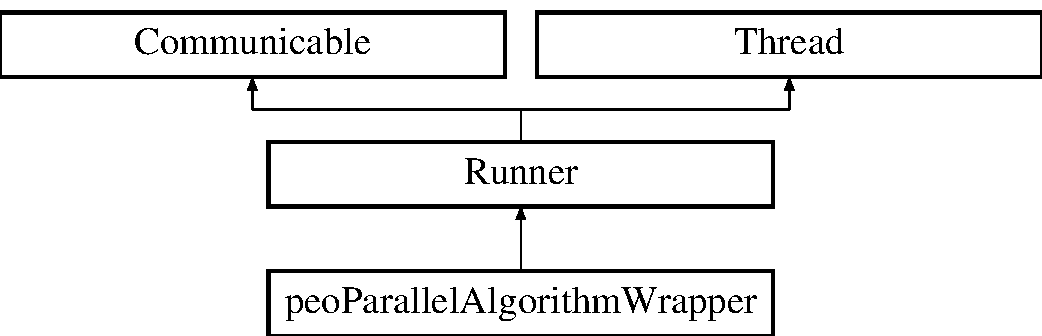
\includegraphics[height=3cm]{classpeoParallelAlgorithmWrapper}
\end{center}
\end{figure}
\subsection*{Public Member Functions}
\begin{CompactItemize}
\item 
\hypertarget{classpeoParallelAlgorithmWrapper_e1e1de8b007934080876df1c65c4d8b0}{
template$<$typename Algorithm\-Type$>$ \hyperlink{classpeoParallelAlgorithmWrapper_e1e1de8b007934080876df1c65c4d8b0}{peo\-Parallel\-Algorithm\-Wrapper} (Algorithm\-Type \&external\-Algorithm)}
\label{classpeoParallelAlgorithmWrapper_e1e1de8b007934080876df1c65c4d8b0}

\item 
\hypertarget{classpeoParallelAlgorithmWrapper_1ebfe70e6826002f6280aba01e141ad5}{
template$<$typename Algorithm\-Type, typename Algorithm\-Data\-Type$>$ \hyperlink{classpeoParallelAlgorithmWrapper_1ebfe70e6826002f6280aba01e141ad5}{peo\-Parallel\-Algorithm\-Wrapper} (Algorithm\-Type \&external\-Algorithm, Algorithm\-Data\-Type \&external\-Data)}
\label{classpeoParallelAlgorithmWrapper_1ebfe70e6826002f6280aba01e141ad5}

\item 
\hypertarget{classpeoParallelAlgorithmWrapper_0e64f517afe790db467750a6980e1666}{
\hyperlink{classpeoParallelAlgorithmWrapper_0e64f517afe790db467750a6980e1666}{$\sim$peo\-Parallel\-Algorithm\-Wrapper} ()}
\label{classpeoParallelAlgorithmWrapper_0e64f517afe790db467750a6980e1666}

\item 
\hypertarget{classpeoParallelAlgorithmWrapper_4b10b46b4ea2e3f66c660c15f3c98e6c}{
void \hyperlink{classpeoParallelAlgorithmWrapper_4b10b46b4ea2e3f66c660c15f3c98e6c}{run} ()}
\label{classpeoParallelAlgorithmWrapper_4b10b46b4ea2e3f66c660c15f3c98e6c}

\end{CompactItemize}
\subsection*{Private Attributes}
\begin{CompactItemize}
\item 
\hypertarget{classpeoParallelAlgorithmWrapper_99f10723f15c63c4822dd6431b9d6d7d}{
\hyperlink{structpeoParallelAlgorithmWrapper_1_1AbstractAlgorithm}{Abstract\-Algorithm} $\ast$ \hyperlink{classpeoParallelAlgorithmWrapper_99f10723f15c63c4822dd6431b9d6d7d}{algorithm}}
\label{classpeoParallelAlgorithmWrapper_99f10723f15c63c4822dd6431b9d6d7d}

\end{CompactItemize}
\subsection*{Classes}
\begin{CompactItemize}
\item 
struct \hyperlink{structpeoParallelAlgorithmWrapper_1_1AbstractAlgorithm}{Abstract\-Algorithm}
\item 
struct \hyperlink{structpeoParallelAlgorithmWrapper_1_1Algorithm}{Algorithm}
\item 
struct \hyperlink{structpeoParallelAlgorithmWrapper_1_1Algorithm_3_01AlgorithmType_00_01void_01_4}{Algorithm$<$ Algorithm\-Type, void $>$}
\end{CompactItemize}


\subsection{Detailed Description}




Definition at line 47 of file peo\-Parallel\-Algorithm\-Wrapper.h.

The documentation for this class was generated from the following file:\begin{CompactItemize}
\item 
peo\-Parallel\-Algorithm\-Wrapper.h\end{CompactItemize}

\hypertarget{structpeoParallelAlgorithmWrapper_1_1AbstractAlgorithm}{
\section{peo\-Parallel\-Algorithm\-Wrapper::Abstract\-Algorithm Struct Reference}
\label{structpeoParallelAlgorithmWrapper_1_1AbstractAlgorithm}\index{peoParallelAlgorithmWrapper::AbstractAlgorithm@{peoParallelAlgorithmWrapper::AbstractAlgorithm}}
}
Inheritance diagram for peo\-Parallel\-Algorithm\-Wrapper::Abstract\-Algorithm::\begin{figure}[H]
\begin{center}
\leavevmode
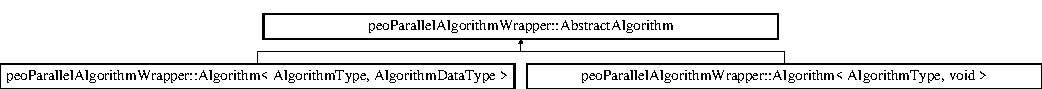
\includegraphics[height=1.20172cm]{structpeoParallelAlgorithmWrapper_1_1AbstractAlgorithm}
\end{center}
\end{figure}
\subsection*{Public Member Functions}
\begin{CompactItemize}
\item 
\hypertarget{structpeoParallelAlgorithmWrapper_1_1AbstractAlgorithm_af530b7731cb212f8dd74e5a57484a9e}{
virtual \hyperlink{structpeoParallelAlgorithmWrapper_1_1AbstractAlgorithm_af530b7731cb212f8dd74e5a57484a9e}{$\sim$Abstract\-Algorithm} ()}
\label{structpeoParallelAlgorithmWrapper_1_1AbstractAlgorithm_af530b7731cb212f8dd74e5a57484a9e}

\item 
\hypertarget{structpeoParallelAlgorithmWrapper_1_1AbstractAlgorithm_32e08b3810cef49d0b8751645ef79b6f}{
virtual void \hyperlink{structpeoParallelAlgorithmWrapper_1_1AbstractAlgorithm_32e08b3810cef49d0b8751645ef79b6f}{operator()} ()}
\label{structpeoParallelAlgorithmWrapper_1_1AbstractAlgorithm_32e08b3810cef49d0b8751645ef79b6f}

\end{CompactItemize}


\subsection{Detailed Description}




Definition at line 71 of file peo\-Parallel\-Algorithm\-Wrapper.h.

The documentation for this struct was generated from the following file:\begin{CompactItemize}
\item 
peo\-Parallel\-Algorithm\-Wrapper.h\end{CompactItemize}

\hypertarget{structpeoParallelAlgorithmWrapper_1_1Algorithm}{
\section{peo\-Parallel\-Algorithm\-Wrapper::Algorithm$<$ Algorithm\-Type, Algorithm\-Data\-Type $>$ Struct Template Reference}
\label{structpeoParallelAlgorithmWrapper_1_1Algorithm}\index{peoParallelAlgorithmWrapper::Algorithm@{peoParallelAlgorithmWrapper::Algorithm}}
}
Inheritance diagram for peo\-Parallel\-Algorithm\-Wrapper::Algorithm$<$ Algorithm\-Type, Algorithm\-Data\-Type $>$::\begin{figure}[H]
\begin{center}
\leavevmode
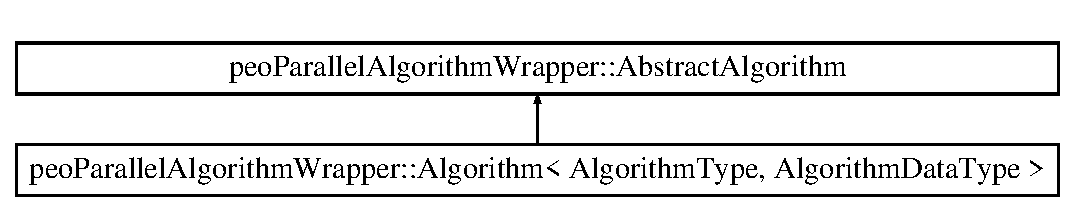
\includegraphics[height=2cm]{structpeoParallelAlgorithmWrapper_1_1Algorithm}
\end{center}
\end{figure}
\subsection*{Public Member Functions}
\begin{CompactItemize}
\item 
\hypertarget{structpeoParallelAlgorithmWrapper_1_1Algorithm_bdd2048610a35f525d7cef9a9041caba}{
\hyperlink{structpeoParallelAlgorithmWrapper_1_1Algorithm_bdd2048610a35f525d7cef9a9041caba}{Algorithm} (Algorithm\-Type \&external\-Algorithm, Algorithm\-Data\-Type \&external\-Data)}
\label{structpeoParallelAlgorithmWrapper_1_1Algorithm_bdd2048610a35f525d7cef9a9041caba}

\item 
\hypertarget{structpeoParallelAlgorithmWrapper_1_1Algorithm_a54fa5366a7663491608399ab21ea092}{
virtual void \hyperlink{structpeoParallelAlgorithmWrapper_1_1Algorithm_a54fa5366a7663491608399ab21ea092}{operator()} ()}
\label{structpeoParallelAlgorithmWrapper_1_1Algorithm_a54fa5366a7663491608399ab21ea092}

\end{CompactItemize}
\subsection*{Public Attributes}
\begin{CompactItemize}
\item 
\hypertarget{structpeoParallelAlgorithmWrapper_1_1Algorithm_91681bf54649f58335c181515a92db7a}{
Algorithm\-Type \& \hyperlink{structpeoParallelAlgorithmWrapper_1_1Algorithm_91681bf54649f58335c181515a92db7a}{algorithm}}
\label{structpeoParallelAlgorithmWrapper_1_1Algorithm_91681bf54649f58335c181515a92db7a}

\item 
\hypertarget{structpeoParallelAlgorithmWrapper_1_1Algorithm_e812277c85c5b6884d2019849e7eabde}{
Algorithm\-Data\-Type \& \hyperlink{structpeoParallelAlgorithmWrapper_1_1Algorithm_e812277c85c5b6884d2019849e7eabde}{algorithm\-Data}}
\label{structpeoParallelAlgorithmWrapper_1_1Algorithm_e812277c85c5b6884d2019849e7eabde}

\end{CompactItemize}


\subsection{Detailed Description}
\subsubsection*{template$<$typename Algorithm\-Type, typename Algorithm\-Data\-Type$>$ struct peo\-Parallel\-Algorithm\-Wrapper::Algorithm$<$ Algorithm\-Type, Algorithm\-Data\-Type $>$}





Definition at line 81 of file peo\-Parallel\-Algorithm\-Wrapper.h.

The documentation for this struct was generated from the following file:\begin{CompactItemize}
\item 
peo\-Parallel\-Algorithm\-Wrapper.h\end{CompactItemize}

\hypertarget{structpeoParallelAlgorithmWrapper_1_1Algorithm_3_01AlgorithmType_00_01void_01_4}{
\section{peo\-Parallel\-Algorithm\-Wrapper::Algorithm$<$ Algorithm\-Type, void $>$ Struct Template Reference}
\label{structpeoParallelAlgorithmWrapper_1_1Algorithm_3_01AlgorithmType_00_01void_01_4}\index{peoParallelAlgorithmWrapper::Algorithm< AlgorithmType, void >@{peoParallelAlgorithmWrapper::Algorithm$<$ AlgorithmType, void $>$}}
}
Inheritance diagram for peo\-Parallel\-Algorithm\-Wrapper::Algorithm$<$ Algorithm\-Type, void $>$::\begin{figure}[H]
\begin{center}
\leavevmode
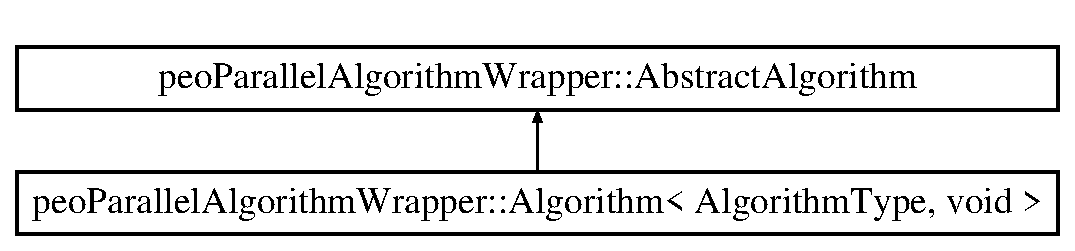
\includegraphics[height=2cm]{structpeoParallelAlgorithmWrapper_1_1Algorithm_3_01AlgorithmType_00_01void_01_4}
\end{center}
\end{figure}
\subsection*{Public Member Functions}
\begin{CompactItemize}
\item 
\hypertarget{structpeoParallelAlgorithmWrapper_1_1Algorithm_3_01AlgorithmType_00_01void_01_4_c44d45b69accab079e1fb30d7ddf6b4e}{
\hyperlink{structpeoParallelAlgorithmWrapper_1_1Algorithm_3_01AlgorithmType_00_01void_01_4_c44d45b69accab079e1fb30d7ddf6b4e}{Algorithm} (Algorithm\-Type \&external\-Algorithm)}
\label{structpeoParallelAlgorithmWrapper_1_1Algorithm_3_01AlgorithmType_00_01void_01_4_c44d45b69accab079e1fb30d7ddf6b4e}

\item 
\hypertarget{structpeoParallelAlgorithmWrapper_1_1Algorithm_3_01AlgorithmType_00_01void_01_4_27b5bd346932e7f3ba9dd8c9e0dd952b}{
virtual void \hyperlink{structpeoParallelAlgorithmWrapper_1_1Algorithm_3_01AlgorithmType_00_01void_01_4_27b5bd346932e7f3ba9dd8c9e0dd952b}{operator()} ()}
\label{structpeoParallelAlgorithmWrapper_1_1Algorithm_3_01AlgorithmType_00_01void_01_4_27b5bd346932e7f3ba9dd8c9e0dd952b}

\end{CompactItemize}
\subsection*{Public Attributes}
\begin{CompactItemize}
\item 
\hypertarget{structpeoParallelAlgorithmWrapper_1_1Algorithm_3_01AlgorithmType_00_01void_01_4_7dcb305dd8c78ffac232bd86b913183d}{
Algorithm\-Type \& \hyperlink{structpeoParallelAlgorithmWrapper_1_1Algorithm_3_01AlgorithmType_00_01void_01_4_7dcb305dd8c78ffac232bd86b913183d}{algorithm}}
\label{structpeoParallelAlgorithmWrapper_1_1Algorithm_3_01AlgorithmType_00_01void_01_4_7dcb305dd8c78ffac232bd86b913183d}

\end{CompactItemize}


\subsection{Detailed Description}
\subsubsection*{template$<$typename Algorithm\-Type$>$ struct peo\-Parallel\-Algorithm\-Wrapper::Algorithm$<$ Algorithm\-Type, void $>$}





Definition at line 95 of file peo\-Parallel\-Algorithm\-Wrapper.h.

The documentation for this struct was generated from the following file:\begin{CompactItemize}
\item 
peo\-Parallel\-Algorithm\-Wrapper.h\end{CompactItemize}

\hypertarget{classpeoParaPopEval}{
\section{peo\-Para\-Pop\-Eval$<$ EOT $>$ Class Template Reference}
\label{classpeoParaPopEval}\index{peoParaPopEval@{peoParaPopEval}}
}
The \hyperlink{classpeoParaPopEval}{peo\-Para\-Pop\-Eval} represents a wrapper for creating a functor capable of applying in parallel an EO-derived evaluation functor.  


{\tt \#include $<$peo\-Para\-Pop\-Eval.h$>$}

Inheritance diagram for peo\-Para\-Pop\-Eval$<$ EOT $>$::\begin{figure}[H]
\begin{center}
\leavevmode
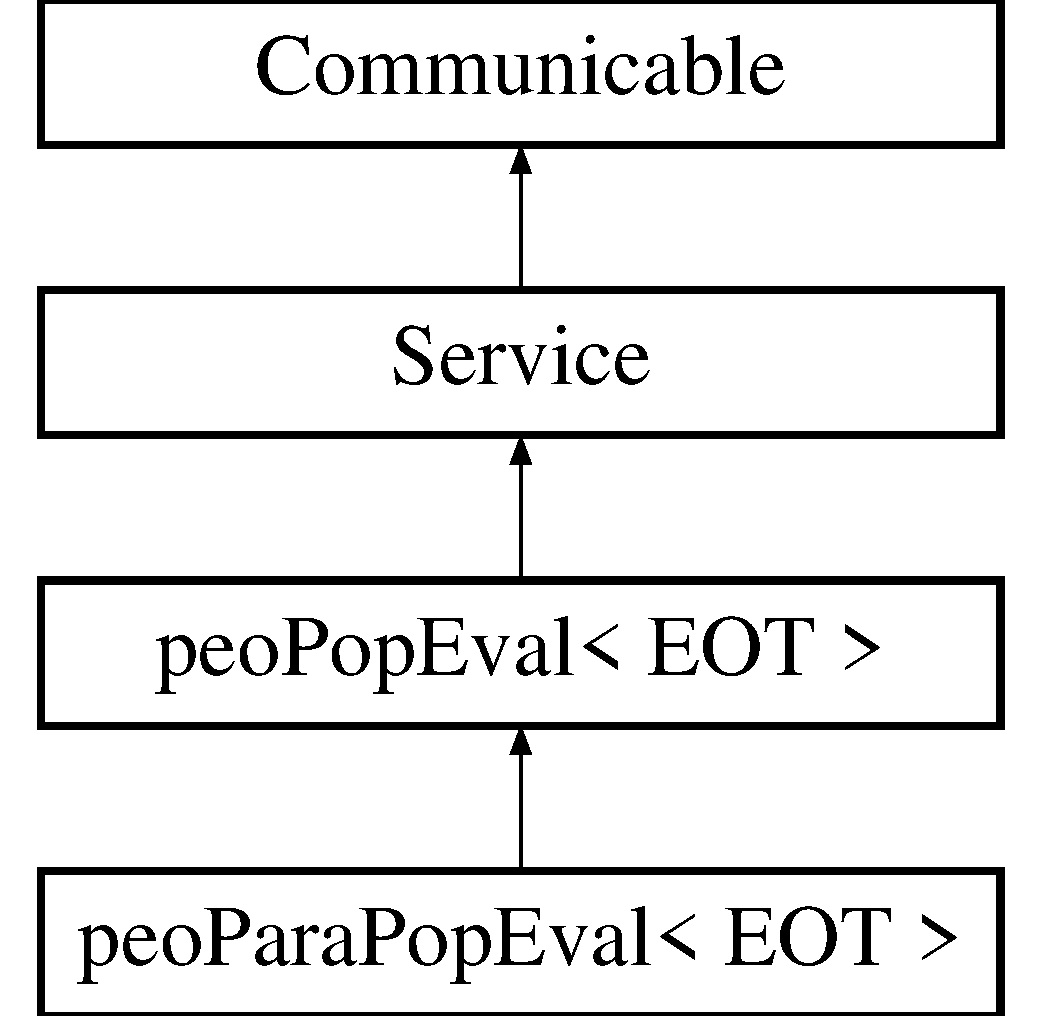
\includegraphics[height=4cm]{classpeoParaPopEval}
\end{center}
\end{figure}
\subsection*{Public Member Functions}
\begin{CompactItemize}
\item 
\hyperlink{classpeoParaPopEval_bcb540510a7038520bec41a7af332daf}{peo\-Para\-Pop\-Eval} (\bf{eo\-Eval\-Func}$<$ EOT $>$ \&\_\-\_\-eval\_\-func)
\begin{CompactList}\small\item\em Constructor function - an EO-derived evaluation functor has to be specified; an internal reference is set towards the specified evaluation functor. \item\end{CompactList}\item 
\hyperlink{classpeoParaPopEval_1cc13a1ec366f95d219d682eccb455bc}{peo\-Para\-Pop\-Eval} (const std::vector$<$ \bf{eo\-Eval\-Func}$<$ EOT $>$ $\ast$ $>$ \&\_\-\_\-funcs, \hyperlink{classpeoAggEvalFunc}{peo\-Agg\-Eval\-Func}$<$ EOT $>$ \&\_\-\_\-merge\_\-eval)
\begin{CompactList}\small\item\em Constructor function - a vector of EO-derived evaluation functors has to be specified as well as an aggregation function. \item\end{CompactList}\item 
void \hyperlink{classpeoParaPopEval_aeaa4fca4f8650e453e308838b4a2cb5}{operator()} (\bf{eo\-Pop}$<$ EOT $>$ \&\_\-\_\-pop)
\begin{CompactList}\small\item\em Operator for applying the evaluation functor (direct or aggregate) for each individual of the specified population. \item\end{CompactList}\item 
void \hyperlink{classpeoParaPopEval_fea632bd645ab11182782fd3c038d6d8}{pack\-Data} ()
\begin{CompactList}\small\item\em Auxiliary function for transferring data between the process requesting an evaluation operation and the process that performs the actual evaluation phase. \item\end{CompactList}\item 
void \hyperlink{classpeoParaPopEval_410bf4c173e2f36df82251cb16ce1b05}{unpack\-Data} ()
\begin{CompactList}\small\item\em Auxiliary function for transferring data between the process requesting an evaluation operation and the process that performs the actual evaluation phase. \item\end{CompactList}\item 
\hypertarget{classpeoParaPopEval_3af76378611eac5a36da9a0a00aeeb6c}{
void \hyperlink{classpeoParaPopEval_3af76378611eac5a36da9a0a00aeeb6c}{execute} ()}
\label{classpeoParaPopEval_3af76378611eac5a36da9a0a00aeeb6c}

\begin{CompactList}\small\item\em Auxiliary function - it calls the specified evaluation functor(s). There is no need to explicitly call the function. \item\end{CompactList}\item 
void \hyperlink{classpeoParaPopEval_24bb4ae84b0b9f64e7170e3d2b0e1223}{pack\-Result} ()
\begin{CompactList}\small\item\em Auxiliary function for transferring data between the process requesting an evaluation operation and the process that performs the actual evaluation phase. \item\end{CompactList}\item 
void \hyperlink{classpeoParaPopEval_fd7f0afe9cba30be39269d16097e190e}{unpack\-Result} ()
\begin{CompactList}\small\item\em Auxiliary function for transferring data between the process requesting an evaluation operation and the process that performs the actual evaluation phase. \item\end{CompactList}\item 
void \hyperlink{classpeoParaPopEval_1f78c3cec2940af08a059cc1aa96a9c8}{notify\-Sending\-Data} ()
\begin{CompactList}\small\item\em Auxiliary function for notifications between the process requesting an evaluation operation and the processes that performs the actual evaluation phase. \item\end{CompactList}\item 
void \hyperlink{classpeoParaPopEval_b77031fc4807921ffaf7cf6b669a7665}{notify\-Sending\-All\-Resource\-Requests} ()
\begin{CompactList}\small\item\em Auxiliary function for notifications between the process requesting an evaluation operation and the processes that performs the actual evaluation phase. \item\end{CompactList}\end{CompactItemize}
\subsection*{Private Attributes}
\begin{CompactItemize}
\item 
\hypertarget{classpeoParaPopEval_6d69b8f73c0b5d72baf75d6e53f025b7}{
const std::vector$<$ \bf{eo\-Eval\-Func}$<$ EOT $>$ $\ast$ $>$ \& \hyperlink{classpeoParaPopEval_6d69b8f73c0b5d72baf75d6e53f025b7}{funcs}}
\label{classpeoParaPopEval_6d69b8f73c0b5d72baf75d6e53f025b7}

\item 
\hypertarget{classpeoParaPopEval_f0e8af3ee442d2b6baf0bd122226be3c}{
std::vector$<$ \bf{eo\-Eval\-Func}$<$ EOT $>$ $\ast$ $>$ \hyperlink{classpeoParaPopEval_f0e8af3ee442d2b6baf0bd122226be3c}{one\_\-func}}
\label{classpeoParaPopEval_f0e8af3ee442d2b6baf0bd122226be3c}

\item 
\hypertarget{classpeoParaPopEval_b48bcd4e9f92f364118304535c089456}{
\hyperlink{classpeoAggEvalFunc}{peo\-Agg\-Eval\-Func}$<$ EOT $>$ \& \hyperlink{classpeoParaPopEval_b48bcd4e9f92f364118304535c089456}{merge\_\-eval}}
\label{classpeoParaPopEval_b48bcd4e9f92f364118304535c089456}

\item 
\hypertarget{classpeoParaPopEval_bf255dd5861e27108c2abae7309d7690}{
\hyperlink{classpeoNoAggEvalFunc}{peo\-No\-Agg\-Eval\-Func}$<$ EOT $>$ \hyperlink{classpeoParaPopEval_bf255dd5861e27108c2abae7309d7690}{no\_\-merge\_\-eval}}
\label{classpeoParaPopEval_bf255dd5861e27108c2abae7309d7690}

\item 
\hypertarget{classpeoParaPopEval_af76cd18368a0f6185878f37f0b5f272}{
std::queue$<$ EOT $\ast$ $>$ \hyperlink{classpeoParaPopEval_af76cd18368a0f6185878f37f0b5f272}{tasks}}
\label{classpeoParaPopEval_af76cd18368a0f6185878f37f0b5f272}

\item 
\hypertarget{classpeoParaPopEval_80e7e34bb1bb2d12f1f2eed3feac6ecf}{
std::map$<$ EOT $\ast$, std::pair$<$ unsigned, unsigned $>$ $>$ \hyperlink{classpeoParaPopEval_80e7e34bb1bb2d12f1f2eed3feac6ecf}{progression}}
\label{classpeoParaPopEval_80e7e34bb1bb2d12f1f2eed3feac6ecf}

\item 
\hypertarget{classpeoParaPopEval_87abb090c0de39f0ccc36af1f07cca0c}{
unsigned \hyperlink{classpeoParaPopEval_87abb090c0de39f0ccc36af1f07cca0c}{num\_\-func}}
\label{classpeoParaPopEval_87abb090c0de39f0ccc36af1f07cca0c}

\item 
\hypertarget{classpeoParaPopEval_fb6941e0455515a908eb82342b995163}{
EOT \hyperlink{classpeoParaPopEval_fb6941e0455515a908eb82342b995163}{sol}}
\label{classpeoParaPopEval_fb6941e0455515a908eb82342b995163}

\item 
\hypertarget{classpeoParaPopEval_60cafeab376262af675fdff43434c8d8}{
EOT $\ast$ \hyperlink{classpeoParaPopEval_60cafeab376262af675fdff43434c8d8}{ad\_\-sol}}
\label{classpeoParaPopEval_60cafeab376262af675fdff43434c8d8}

\item 
\hypertarget{classpeoParaPopEval_b528ad9dd9006c3dd57f149a3843e57d}{
unsigned \hyperlink{classpeoParaPopEval_b528ad9dd9006c3dd57f149a3843e57d}{total}}
\label{classpeoParaPopEval_b528ad9dd9006c3dd57f149a3843e57d}

\end{CompactItemize}


\subsection{Detailed Description}
\subsubsection*{template$<$class EOT$>$ class peo\-Para\-Pop\-Eval$<$ EOT $>$}

The \hyperlink{classpeoParaPopEval}{peo\-Para\-Pop\-Eval} represents a wrapper for creating a functor capable of applying in parallel an EO-derived evaluation functor. 

The class offers the possibility of chosing between a single-function evaluation and an aggregate evaluation function, including several sub-evalution functions. 



Definition at line 54 of file peo\-Para\-Pop\-Eval.h.

\subsection{Constructor \& Destructor Documentation}
\hypertarget{classpeoParaPopEval_bcb540510a7038520bec41a7af332daf}{
\index{peoParaPopEval@{peo\-Para\-Pop\-Eval}!peoParaPopEval@{peoParaPopEval}}
\index{peoParaPopEval@{peoParaPopEval}!peoParaPopEval@{peo\-Para\-Pop\-Eval}}
\subsubsection[peoParaPopEval]{\setlength{\rightskip}{0pt plus 5cm}template$<$class EOT$>$ \hyperlink{classpeoParaPopEval}{peo\-Para\-Pop\-Eval}$<$ EOT $>$::\hyperlink{classpeoParaPopEval}{peo\-Para\-Pop\-Eval} (\bf{eo\-Eval\-Func}$<$ EOT $>$ \& {\em \_\-\_\-eval\_\-func})}}
\label{classpeoParaPopEval_bcb540510a7038520bec41a7af332daf}


Constructor function - an EO-derived evaluation functor has to be specified; an internal reference is set towards the specified evaluation functor. 

\begin{Desc}
\item[Parameters:]
\begin{description}
\item[{\em eo\-Eval\-Func$<$}]EOT $>$\& \_\-\_\-eval\_\-func - EO-derived evaluation functor to be applied in parallel on each individual of a specified population \end{description}
\end{Desc}


Definition at line 130 of file peo\-Para\-Pop\-Eval.h.

References peo\-Para\-Pop\-Eval$<$ EOT $>$::one\_\-func.\hypertarget{classpeoParaPopEval_1cc13a1ec366f95d219d682eccb455bc}{
\index{peoParaPopEval@{peo\-Para\-Pop\-Eval}!peoParaPopEval@{peoParaPopEval}}
\index{peoParaPopEval@{peoParaPopEval}!peoParaPopEval@{peo\-Para\-Pop\-Eval}}
\subsubsection[peoParaPopEval]{\setlength{\rightskip}{0pt plus 5cm}template$<$class EOT$>$ \hyperlink{classpeoParaPopEval}{peo\-Para\-Pop\-Eval}$<$ EOT $>$::\hyperlink{classpeoParaPopEval}{peo\-Para\-Pop\-Eval} (const std::vector$<$ \bf{eo\-Eval\-Func}$<$ EOT $>$ $\ast$ $>$ \& {\em \_\-\_\-funcs}, \hyperlink{classpeoAggEvalFunc}{peo\-Agg\-Eval\-Func}$<$ EOT $>$ \& {\em \_\-\_\-merge\_\-eval})}}
\label{classpeoParaPopEval_1cc13a1ec366f95d219d682eccb455bc}


Constructor function - a vector of EO-derived evaluation functors has to be specified as well as an aggregation function. 

\begin{Desc}
\item[Parameters:]
\begin{description}
\item[{\em const}]std :: vector$<$ \doxyref{eo\-Eval\-Func} $<$ EOT $>$$\ast$ $>$\& \_\-\_\-funcs - vector of EO-derived partial evaluation functors; \item[{\em peo\-Agg\-Eval\-Func$<$}]EOT $>$\& \_\-\_\-merge\_\-eval - aggregation functor for creating a fitness value out of the partial fitness values. \end{description}
\end{Desc}


Definition at line 139 of file peo\-Para\-Pop\-Eval.h.

\subsection{Member Function Documentation}
\hypertarget{classpeoParaPopEval_aeaa4fca4f8650e453e308838b4a2cb5}{
\index{peoParaPopEval@{peo\-Para\-Pop\-Eval}!operator()@{operator()}}
\index{operator()@{operator()}!peoParaPopEval@{peo\-Para\-Pop\-Eval}}
\subsubsection[operator()]{\setlength{\rightskip}{0pt plus 5cm}template$<$class EOT$>$ void \hyperlink{classpeoParaPopEval}{peo\-Para\-Pop\-Eval}$<$ EOT $>$::operator() (\bf{eo\-Pop}$<$ EOT $>$ \& {\em \_\-\_\-pop})\hspace{0.3cm}{\tt  \mbox{[}virtual\mbox{]}}}}
\label{classpeoParaPopEval_aeaa4fca4f8650e453e308838b4a2cb5}


Operator for applying the evaluation functor (direct or aggregate) for each individual of the specified population. 

\begin{Desc}
\item[Parameters:]
\begin{description}
\item[{\em eo\-Pop$<$}]EOT $>$\& \_\-\_\-pop - population to be evaluated by applying the evaluation functor specified in the constructor. \end{description}
\end{Desc}


Implements \hyperlink{classpeoPopEval_2f208067a5e39c3b26c1234050a41e8f}{peo\-Pop\-Eval$<$ EOT $>$}.

Definition at line 150 of file peo\-Para\-Pop\-Eval.h.

References peo\-Para\-Pop\-Eval$<$ EOT $>$::funcs, peo\-Para\-Pop\-Eval$<$ EOT $>$::progression, Service::request\-Resource\-Request(), Communicable::stop(), peo\-Para\-Pop\-Eval$<$ EOT $>$::tasks, and peo\-Para\-Pop\-Eval$<$ EOT $>$::total.\hypertarget{classpeoParaPopEval_fea632bd645ab11182782fd3c038d6d8}{
\index{peoParaPopEval@{peo\-Para\-Pop\-Eval}!packData@{packData}}
\index{packData@{packData}!peoParaPopEval@{peo\-Para\-Pop\-Eval}}
\subsubsection[packData]{\setlength{\rightskip}{0pt plus 5cm}template$<$class EOT$>$ void \hyperlink{classpeoParaPopEval}{peo\-Para\-Pop\-Eval}$<$ EOT $>$::pack\-Data ()\hspace{0.3cm}{\tt  \mbox{[}virtual\mbox{]}}}}
\label{classpeoParaPopEval_fea632bd645ab11182782fd3c038d6d8}


Auxiliary function for transferring data between the process requesting an evaluation operation and the process that performs the actual evaluation phase. 

There is no need to explicitly call the function. 

Reimplemented from \hyperlink{classService_aea4b8f7f8fb88e83862ee4bfd9ab207}{Service}.

Definition at line 171 of file peo\-Para\-Pop\-Eval.h.

References peo\-Para\-Pop\-Eval$<$ EOT $>$::progression, and peo\-Para\-Pop\-Eval$<$ EOT $>$::tasks.\hypertarget{classpeoParaPopEval_410bf4c173e2f36df82251cb16ce1b05}{
\index{peoParaPopEval@{peo\-Para\-Pop\-Eval}!unpackData@{unpackData}}
\index{unpackData@{unpackData}!peoParaPopEval@{peo\-Para\-Pop\-Eval}}
\subsubsection[unpackData]{\setlength{\rightskip}{0pt plus 5cm}template$<$class EOT$>$ void \hyperlink{classpeoParaPopEval}{peo\-Para\-Pop\-Eval}$<$ EOT $>$::unpack\-Data ()\hspace{0.3cm}{\tt  \mbox{[}virtual\mbox{]}}}}
\label{classpeoParaPopEval_410bf4c173e2f36df82251cb16ce1b05}


Auxiliary function for transferring data between the process requesting an evaluation operation and the process that performs the actual evaluation phase. 

There is no need to explicitly call the function. 

Reimplemented from \hyperlink{classService_3bd87b444710813d30fd754d4d0b4df3}{Service}.

Definition at line 185 of file peo\-Para\-Pop\-Eval.h.

References peo\-Para\-Pop\-Eval$<$ EOT $>$::ad\_\-sol, peo\-Para\-Pop\-Eval$<$ EOT $>$::num\_\-func, and peo\-Para\-Pop\-Eval$<$ EOT $>$::sol.\hypertarget{classpeoParaPopEval_24bb4ae84b0b9f64e7170e3d2b0e1223}{
\index{peoParaPopEval@{peo\-Para\-Pop\-Eval}!packResult@{packResult}}
\index{packResult@{packResult}!peoParaPopEval@{peo\-Para\-Pop\-Eval}}
\subsubsection[packResult]{\setlength{\rightskip}{0pt plus 5cm}template$<$class EOT$>$ void \hyperlink{classpeoParaPopEval}{peo\-Para\-Pop\-Eval}$<$ EOT $>$::pack\-Result ()\hspace{0.3cm}{\tt  \mbox{[}virtual\mbox{]}}}}
\label{classpeoParaPopEval_24bb4ae84b0b9f64e7170e3d2b0e1223}


Auxiliary function for transferring data between the process requesting an evaluation operation and the process that performs the actual evaluation phase. 

There is no need to explicitly call the function. 

Reimplemented from \hyperlink{classService_e5e4f90b2315e15c2a2913bd370f4cf5}{Service}.

Definition at line 202 of file peo\-Para\-Pop\-Eval.h.

References peo\-Para\-Pop\-Eval$<$ EOT $>$::ad\_\-sol, and peo\-Para\-Pop\-Eval$<$ EOT $>$::sol.\hypertarget{classpeoParaPopEval_fd7f0afe9cba30be39269d16097e190e}{
\index{peoParaPopEval@{peo\-Para\-Pop\-Eval}!unpackResult@{unpackResult}}
\index{unpackResult@{unpackResult}!peoParaPopEval@{peo\-Para\-Pop\-Eval}}
\subsubsection[unpackResult]{\setlength{\rightskip}{0pt plus 5cm}template$<$class EOT$>$ void \hyperlink{classpeoParaPopEval}{peo\-Para\-Pop\-Eval}$<$ EOT $>$::unpack\-Result ()\hspace{0.3cm}{\tt  \mbox{[}virtual\mbox{]}}}}
\label{classpeoParaPopEval_fd7f0afe9cba30be39269d16097e190e}


Auxiliary function for transferring data between the process requesting an evaluation operation and the process that performs the actual evaluation phase. 

There is no need to explicitly call the function. 

Reimplemented from \hyperlink{classService_45c06344edbfa482b91f68e2035a6099}{Service}.

Definition at line 211 of file peo\-Para\-Pop\-Eval.h.

References peo\-Para\-Pop\-Eval$<$ EOT $>$::ad\_\-sol, Service::get\-Owner(), peo\-Para\-Pop\-Eval$<$ EOT $>$::merge\_\-eval, peo\-Para\-Pop\-Eval$<$ EOT $>$::progression, Communicable::resume(), Thread::set\-Active(), and peo\-Para\-Pop\-Eval$<$ EOT $>$::total.\hypertarget{classpeoParaPopEval_1f78c3cec2940af08a059cc1aa96a9c8}{
\index{peoParaPopEval@{peo\-Para\-Pop\-Eval}!notifySendingData@{notifySendingData}}
\index{notifySendingData@{notifySendingData}!peoParaPopEval@{peo\-Para\-Pop\-Eval}}
\subsubsection[notifySendingData]{\setlength{\rightskip}{0pt plus 5cm}template$<$class EOT$>$ void \hyperlink{classpeoParaPopEval}{peo\-Para\-Pop\-Eval}$<$ EOT $>$::notify\-Sending\-Data ()\hspace{0.3cm}{\tt  \mbox{[}virtual\mbox{]}}}}
\label{classpeoParaPopEval_1f78c3cec2940af08a059cc1aa96a9c8}


Auxiliary function for notifications between the process requesting an evaluation operation and the processes that performs the actual evaluation phase. 

There is no need to explicitly call the function. 

Reimplemented from \hyperlink{classService_81ad4d6ebb50045b8977e2ab74826f30}{Service}.

Definition at line 242 of file peo\-Para\-Pop\-Eval.h.\hypertarget{classpeoParaPopEval_b77031fc4807921ffaf7cf6b669a7665}{
\index{peoParaPopEval@{peo\-Para\-Pop\-Eval}!notifySendingAllResourceRequests@{notifySendingAllResourceRequests}}
\index{notifySendingAllResourceRequests@{notifySendingAllResourceRequests}!peoParaPopEval@{peo\-Para\-Pop\-Eval}}
\subsubsection[notifySendingAllResourceRequests]{\setlength{\rightskip}{0pt plus 5cm}template$<$class EOT$>$ void \hyperlink{classpeoParaPopEval}{peo\-Para\-Pop\-Eval}$<$ EOT $>$::notify\-Sending\-All\-Resource\-Requests ()\hspace{0.3cm}{\tt  \mbox{[}virtual\mbox{]}}}}
\label{classpeoParaPopEval_b77031fc4807921ffaf7cf6b669a7665}


Auxiliary function for notifications between the process requesting an evaluation operation and the processes that performs the actual evaluation phase. 

There is no need to explicitly call the function. 

Reimplemented from \hyperlink{classService_f94cc8a5c2665d4574041737e61e9ffc}{Service}.

Definition at line 247 of file peo\-Para\-Pop\-Eval.h.

References Service::get\-Owner(), and Thread::set\-Passive().

The documentation for this class was generated from the following file:\begin{CompactItemize}
\item 
peo\-Para\-Pop\-Eval.h\end{CompactItemize}

\hypertarget{classpeoParaSGATransform}{
\section{peo\-Para\-SGATransform$<$ EOT $>$ Class Template Reference}
\label{classpeoParaSGATransform}\index{peoParaSGATransform@{peoParaSGATransform}}
}
Inheritance diagram for peo\-Para\-SGATransform$<$ EOT $>$::\begin{figure}[H]
\begin{center}
\leavevmode
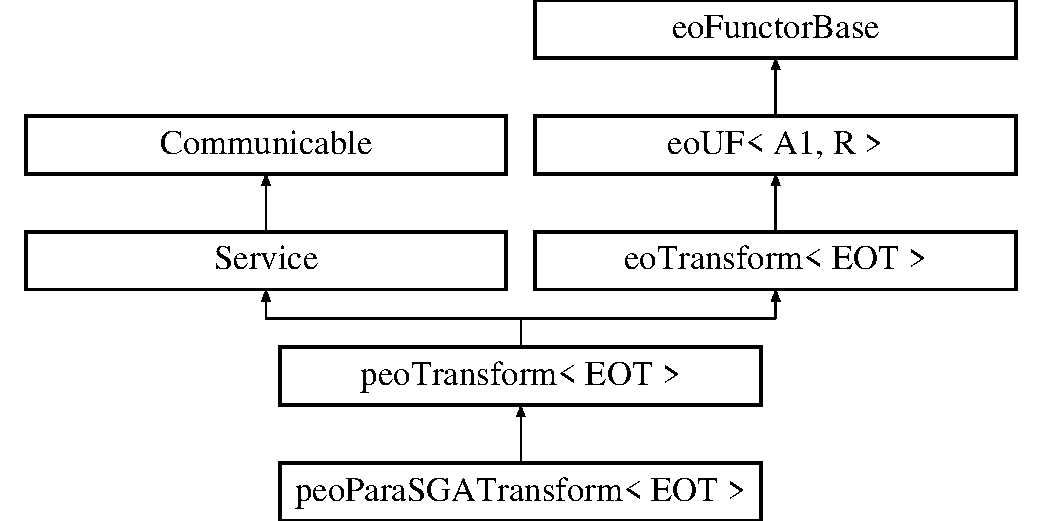
\includegraphics[height=5cm]{classpeoParaSGATransform}
\end{center}
\end{figure}
\subsection*{Public Member Functions}
\begin{CompactItemize}
\item 
\hypertarget{classpeoParaSGATransform_2052bca82fbbfe5455bf6f69246d4dbf}{
\hyperlink{classpeoParaSGATransform_2052bca82fbbfe5455bf6f69246d4dbf}{peo\-Para\-SGATransform} (\bf{eo\-Quad\-Op}$<$ EOT $>$ \&\_\-\_\-cross, double \_\-\_\-cross\_\-rate, \bf{eo\-Mon\-Op}$<$ EOT $>$ \&\_\-\_\-mut, double \_\-\_\-mut\_\-rate)}
\label{classpeoParaSGATransform_2052bca82fbbfe5455bf6f69246d4dbf}

\item 
\hypertarget{classpeoParaSGATransform_669de7f7c6316fa745a15b909efb6527}{
void \hyperlink{classpeoParaSGATransform_669de7f7c6316fa745a15b909efb6527}{operator()} (\bf{eo\-Pop}$<$ EOT $>$ \&\_\-\_\-pop)}
\label{classpeoParaSGATransform_669de7f7c6316fa745a15b909efb6527}

\item 
\hypertarget{classpeoParaSGATransform_fd278bcde58d29c9a343d5cbead81a1e}{
void \hyperlink{classpeoParaSGATransform_fd278bcde58d29c9a343d5cbead81a1e}{pack\-Data} ()}
\label{classpeoParaSGATransform_fd278bcde58d29c9a343d5cbead81a1e}

\item 
\hypertarget{classpeoParaSGATransform_a43a487a6e81791c8bbf6ce30f4336ab}{
void \hyperlink{classpeoParaSGATransform_a43a487a6e81791c8bbf6ce30f4336ab}{unpack\-Data} ()}
\label{classpeoParaSGATransform_a43a487a6e81791c8bbf6ce30f4336ab}

\item 
\hypertarget{classpeoParaSGATransform_c9de2100fb897177a401c634002f6dd9}{
void \hyperlink{classpeoParaSGATransform_c9de2100fb897177a401c634002f6dd9}{execute} ()}
\label{classpeoParaSGATransform_c9de2100fb897177a401c634002f6dd9}

\item 
\hypertarget{classpeoParaSGATransform_ba08e224ceaa4149e8e1a88694a2ccf2}{
void \hyperlink{classpeoParaSGATransform_ba08e224ceaa4149e8e1a88694a2ccf2}{pack\-Result} ()}
\label{classpeoParaSGATransform_ba08e224ceaa4149e8e1a88694a2ccf2}

\item 
\hypertarget{classpeoParaSGATransform_257663dcdc6cc95b6183d472ffba1b2f}{
void \hyperlink{classpeoParaSGATransform_257663dcdc6cc95b6183d472ffba1b2f}{unpack\-Result} ()}
\label{classpeoParaSGATransform_257663dcdc6cc95b6183d472ffba1b2f}

\item 
\hypertarget{classpeoParaSGATransform_4e19dfc22b6f69fa8b93537226551866}{
void \hyperlink{classpeoParaSGATransform_4e19dfc22b6f69fa8b93537226551866}{notify\-Sending\-Data} ()}
\label{classpeoParaSGATransform_4e19dfc22b6f69fa8b93537226551866}

\item 
\hypertarget{classpeoParaSGATransform_8a0316e33897c395a81787f59ea7a1c8}{
void \hyperlink{classpeoParaSGATransform_8a0316e33897c395a81787f59ea7a1c8}{notify\-Sending\-All\-Resource\-Requests} ()}
\label{classpeoParaSGATransform_8a0316e33897c395a81787f59ea7a1c8}

\end{CompactItemize}
\subsection*{Private Attributes}
\begin{CompactItemize}
\item 
\hypertarget{classpeoParaSGATransform_c6f97deabe7502c84f5b6c479013f6dc}{
\bf{eo\-Quad\-Op}$<$ EOT $>$ \& \hyperlink{classpeoParaSGATransform_c6f97deabe7502c84f5b6c479013f6dc}{cross}}
\label{classpeoParaSGATransform_c6f97deabe7502c84f5b6c479013f6dc}

\item 
\hypertarget{classpeoParaSGATransform_dfcf216e2df05016db4d57a5ffb0b0e2}{
double \hyperlink{classpeoParaSGATransform_dfcf216e2df05016db4d57a5ffb0b0e2}{cross\_\-rate}}
\label{classpeoParaSGATransform_dfcf216e2df05016db4d57a5ffb0b0e2}

\item 
\hypertarget{classpeoParaSGATransform_34ff5f9d285ca4879cf8865fb425a311}{
\bf{eo\-Mon\-Op}$<$ EOT $>$ \& \hyperlink{classpeoParaSGATransform_34ff5f9d285ca4879cf8865fb425a311}{mut}}
\label{classpeoParaSGATransform_34ff5f9d285ca4879cf8865fb425a311}

\item 
\hypertarget{classpeoParaSGATransform_b9d3a2094737d0bbd034aac942cc53e3}{
double \hyperlink{classpeoParaSGATransform_b9d3a2094737d0bbd034aac942cc53e3}{mut\_\-rate}}
\label{classpeoParaSGATransform_b9d3a2094737d0bbd034aac942cc53e3}

\item 
\hypertarget{classpeoParaSGATransform_03972feadc86626e58fe60bd4061b57e}{
unsigned \hyperlink{classpeoParaSGATransform_03972feadc86626e58fe60bd4061b57e}{idx}}
\label{classpeoParaSGATransform_03972feadc86626e58fe60bd4061b57e}

\item 
\hypertarget{classpeoParaSGATransform_94e10a1285e128aba6e71517c941f961}{
\bf{eo\-Pop}$<$ EOT $>$ $\ast$ \hyperlink{classpeoParaSGATransform_94e10a1285e128aba6e71517c941f961}{pop}}
\label{classpeoParaSGATransform_94e10a1285e128aba6e71517c941f961}

\item 
\hypertarget{classpeoParaSGATransform_9ef60190e2e3bd5961a93d1b52cb275d}{
EOT \hyperlink{classpeoParaSGATransform_9ef60190e2e3bd5961a93d1b52cb275d}{father}}
\label{classpeoParaSGATransform_9ef60190e2e3bd5961a93d1b52cb275d}

\item 
\hypertarget{classpeoParaSGATransform_e991ad2af6d116afd855de2db46e1d27}{
EOT \hyperlink{classpeoParaSGATransform_e991ad2af6d116afd855de2db46e1d27}{mother}}
\label{classpeoParaSGATransform_e991ad2af6d116afd855de2db46e1d27}

\item 
\hypertarget{classpeoParaSGATransform_589ea7cd72d522ae51a07de4d8ffbf11}{
unsigned \hyperlink{classpeoParaSGATransform_589ea7cd72d522ae51a07de4d8ffbf11}{num\_\-term}}
\label{classpeoParaSGATransform_589ea7cd72d522ae51a07de4d8ffbf11}

\end{CompactItemize}


\subsection{Detailed Description}
\subsubsection*{template$<$class EOT$>$ class peo\-Para\-SGATransform$<$ EOT $>$}





Definition at line 49 of file peo\-Para\-SGATransform.h.

The documentation for this class was generated from the following file:\begin{CompactItemize}
\item 
peo\-Para\-SGATransform.h\end{CompactItemize}

\hypertarget{classpeoPopEval}{
\section{peo\-Pop\-Eval$<$ EOT $>$ Class Template Reference}
\label{classpeoPopEval}\index{peoPopEval@{peoPopEval}}
}
Parallel evaluation functor wrapper with MOEO.  


{\tt \#include $<$peo\-Moeo\-Pop\-Eval.h$>$}

Inheritance diagram for peo\-Pop\-Eval$<$ EOT $>$::\begin{figure}[H]
\begin{center}
\leavevmode
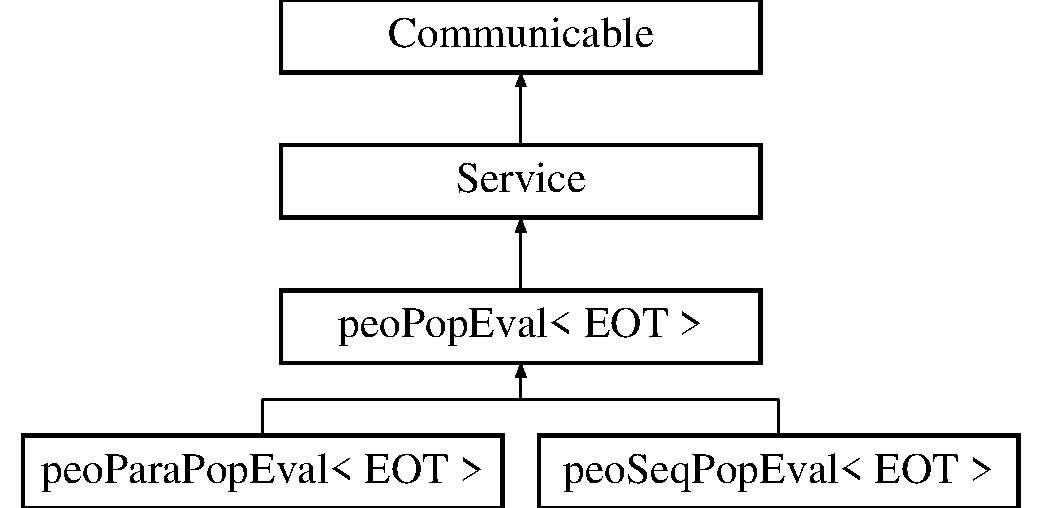
\includegraphics[height=3cm]{classpeoPopEval}
\end{center}
\end{figure}
\subsection*{Public Member Functions}
\begin{CompactItemize}
\item 
\hyperlink{classpeoPopEval_878297ba0de14593bd9cc03b2daf52df}{peo\-Pop\-Eval} (eo\-Eval\-Func$<$ EOT $>$ \&\_\-\_\-eval\_\-func)
\begin{CompactList}\small\item\em Constructor function - an EO-derived evaluation functor has to be specified; an internal reference is set towards the specified evaluation functor. \item\end{CompactList}\item 
\hyperlink{classpeoPopEval_088822da7a0c92bc21574358d2e5f87c}{peo\-Pop\-Eval} (const std::vector$<$ eo\-Eval\-Func$<$ EOT $>$ $\ast$ $>$ \&\_\-\_\-funcs, \hyperlink{classpeoAggEvalFunc}{peo\-Agg\-Eval\-Func}$<$ EOT $>$ \&\_\-\_\-merge\_\-eval)
\begin{CompactList}\small\item\em Constructor function - a vector of EO-derived evaluation functors has to be specified as well as an aggregation function. \item\end{CompactList}\item 
void \hyperlink{classpeoPopEval_593dd60fc004edea8994d5575bf66e05}{operator()} (eo\-Pop$<$ EOT $>$ \&\_\-\_\-pop)
\begin{CompactList}\small\item\em Operator for applying the evaluation functor (direct or aggregate) for each individual of the specified population. \item\end{CompactList}\item 
void \hyperlink{classpeoPopEval_fd942c2b66f31c7d12a9ad48f1529a16}{operator()} (eo\-Pop$<$ EOT $>$ \&\_\-\_\-dummy, eo\-Pop$<$ EOT $>$ \&\_\-\_\-pop)
\item 
void \hyperlink{classpeoPopEval_95351dcd81d1bf878d839e52a02a902d}{pack\-Data} ()
\begin{CompactList}\small\item\em Auxiliary function for transferring data between the process requesting an evaluation operation and the process that performs the actual evaluation phase. \item\end{CompactList}\item 
void \hyperlink{classpeoPopEval_cb256d94000a47af06d3e8a3f7ab0eff}{unpack\-Data} ()
\begin{CompactList}\small\item\em Auxiliary function for transferring data between the process requesting an evaluation operation and the process that performs the actual evaluation phase. \item\end{CompactList}\item 
\hypertarget{classpeoPopEval_05a85a265971d4b12f2f0014d33f705c}{
void \hyperlink{classpeoPopEval_05a85a265971d4b12f2f0014d33f705c}{execute} ()}
\label{classpeoPopEval_05a85a265971d4b12f2f0014d33f705c}

\begin{CompactList}\small\item\em Auxiliary function - it calls the specified evaluation functor(s). There is no need to explicitly call the function. \item\end{CompactList}\item 
void \hyperlink{classpeoPopEval_9d0d10865d677c1ec84f496bed62a8c6}{pack\-Result} ()
\begin{CompactList}\small\item\em Auxiliary function for transferring data between the process requesting an evaluation operation and the process that performs the actual evaluation phase. \item\end{CompactList}\item 
void \hyperlink{classpeoPopEval_f64aa1322e8e26f39143e1a6395206b6}{unpack\-Result} ()
\begin{CompactList}\small\item\em Auxiliary function for transferring data between the process requesting an evaluation operation and the process that performs the actual evaluation phase. \item\end{CompactList}\item 
void \hyperlink{classpeoPopEval_9708f67fc813d397de3d13830ed09820}{notify\-Sending\-Data} ()
\begin{CompactList}\small\item\em Auxiliary function for notifications between the process requesting an evaluation operation and the processes that performs the actual evaluation phase. \item\end{CompactList}\item 
void \hyperlink{classpeoPopEval_b1e33394ba9797237cb8c7c1f410bd67}{notify\-Sending\-All\-Resource\-Requests} ()
\begin{CompactList}\small\item\em Auxiliary function for notifications between the process requesting an evaluation operation and the processes that performs the actual evaluation phase. \item\end{CompactList}\end{CompactItemize}
\subsection*{Private Attributes}
\begin{CompactItemize}
\item 
const std::vector$<$ eo\-Eval\-Func$<$ EOT $>$ $\ast$ $>$ \& \hyperlink{classpeoPopEval_5862b3661c5b0531d55870b5f3881d1e}{funcs}
\item 
\hypertarget{classpeoPopEval_4c563a67b776d97b25a05013ddc99921}{
std::vector$<$ eo\-Eval\-Func$<$ EOT $>$ $\ast$ $>$ \hyperlink{classpeoPopEval_4c563a67b776d97b25a05013ddc99921}{one\_\-func}}
\label{classpeoPopEval_4c563a67b776d97b25a05013ddc99921}

\item 
\hypertarget{classpeoPopEval_765f1941fcb630b6ed5c4cf0e1e845f9}{
\hyperlink{classpeoAggEvalFunc}{peo\-Agg\-Eval\-Func}$<$ EOT $>$ \& \hyperlink{classpeoPopEval_765f1941fcb630b6ed5c4cf0e1e845f9}{merge\_\-eval}}
\label{classpeoPopEval_765f1941fcb630b6ed5c4cf0e1e845f9}

\item 
\hypertarget{classpeoPopEval_8558f626aca54bdc3bbeb78c774ca4ef}{
\hyperlink{classpeoNoAggEvalFunc}{peo\-No\-Agg\-Eval\-Func}$<$ EOT $>$ \hyperlink{classpeoPopEval_8558f626aca54bdc3bbeb78c774ca4ef}{no\_\-merge\_\-eval}}
\label{classpeoPopEval_8558f626aca54bdc3bbeb78c774ca4ef}

\item 
\hypertarget{classpeoPopEval_fc1e9fba1a220550c332c70250f775cc}{
std::queue$<$ EOT $\ast$ $>$ \hyperlink{classpeoPopEval_fc1e9fba1a220550c332c70250f775cc}{tasks}}
\label{classpeoPopEval_fc1e9fba1a220550c332c70250f775cc}

\item 
\hypertarget{classpeoPopEval_25646d6ec0df9f281b17d96956d2201f}{
std::map$<$ EOT $\ast$, std::pair$<$ unsigned, unsigned $>$ $>$ \hyperlink{classpeoPopEval_25646d6ec0df9f281b17d96956d2201f}{progression}}
\label{classpeoPopEval_25646d6ec0df9f281b17d96956d2201f}

\item 
\hypertarget{classpeoPopEval_a6753e36522ece615fb44f91b2986dc6}{
unsigned \hyperlink{classpeoPopEval_a6753e36522ece615fb44f91b2986dc6}{num\_\-func}}
\label{classpeoPopEval_a6753e36522ece615fb44f91b2986dc6}

\item 
\hypertarget{classpeoPopEval_d2bb78c4092b2f57a70fa6f90354ea91}{
EOT \hyperlink{classpeoPopEval_d2bb78c4092b2f57a70fa6f90354ea91}{sol}}
\label{classpeoPopEval_d2bb78c4092b2f57a70fa6f90354ea91}

\item 
\hypertarget{classpeoPopEval_140a0ffb2a481238dde05e7f0324d516}{
EOT $\ast$ \hyperlink{classpeoPopEval_140a0ffb2a481238dde05e7f0324d516}{ad\_\-sol}}
\label{classpeoPopEval_140a0ffb2a481238dde05e7f0324d516}

\item 
\hypertarget{classpeoPopEval_83b38d0977e5c8666c5aa5293c53bb3e}{
unsigned \hyperlink{classpeoPopEval_83b38d0977e5c8666c5aa5293c53bb3e}{total}}
\label{classpeoPopEval_83b38d0977e5c8666c5aa5293c53bb3e}

\end{CompactItemize}


\subsection{Detailed Description}
\subsubsection*{template$<$class EOT$>$ class peo\-Pop\-Eval$<$ EOT $>$}

Parallel evaluation functor wrapper with MOEO. 

\begin{Desc}
\item[See also:]\hyperlink{classService}{Service} eo\-Pop\-Eval\-Func \end{Desc}
\begin{Desc}
\item[Version:]1.0 \end{Desc}
\begin{Desc}
\item[Date:]2008 \end{Desc}




Definition at line 53 of file peo\-Pop\-Eval.h.

\subsection{Constructor \& Destructor Documentation}
\hypertarget{classpeoPopEval_878297ba0de14593bd9cc03b2daf52df}{
\index{peoPopEval@{peo\-Pop\-Eval}!peoPopEval@{peoPopEval}}
\index{peoPopEval@{peoPopEval}!peoPopEval@{peo\-Pop\-Eval}}
\subsubsection[peoPopEval]{\setlength{\rightskip}{0pt plus 5cm}template$<$class EOT$>$ \hyperlink{classpeoPopEval}{peo\-Pop\-Eval}$<$ EOT $>$::\hyperlink{classpeoPopEval}{peo\-Pop\-Eval} (eo\-Eval\-Func$<$ EOT $>$ \& {\em \_\-\_\-eval\_\-func})}}
\label{classpeoPopEval_878297ba0de14593bd9cc03b2daf52df}


Constructor function - an EO-derived evaluation functor has to be specified; an internal reference is set towards the specified evaluation functor. 

\begin{Desc}
\item[Parameters:]
\begin{description}
\item[{\em eo\-Eval\-Func$<$}]EOT $>$\& \_\-\_\-eval\_\-func - EO-derived evaluation functor to be applied in parallel on each individual of a specified population \end{description}
\end{Desc}


Definition at line 132 of file peo\-Pop\-Eval.h.

References peo\-Pop\-Eval$<$ EOT $>$::one\_\-func.\hypertarget{classpeoPopEval_088822da7a0c92bc21574358d2e5f87c}{
\index{peoPopEval@{peo\-Pop\-Eval}!peoPopEval@{peoPopEval}}
\index{peoPopEval@{peoPopEval}!peoPopEval@{peo\-Pop\-Eval}}
\subsubsection[peoPopEval]{\setlength{\rightskip}{0pt plus 5cm}template$<$class EOT$>$ \hyperlink{classpeoPopEval}{peo\-Pop\-Eval}$<$ EOT $>$::\hyperlink{classpeoPopEval}{peo\-Pop\-Eval} (const std::vector$<$ eo\-Eval\-Func$<$ EOT $>$ $\ast$ $>$ \& {\em \_\-\_\-funcs}, \hyperlink{classpeoAggEvalFunc}{peo\-Agg\-Eval\-Func}$<$ EOT $>$ \& {\em \_\-\_\-merge\_\-eval})}}
\label{classpeoPopEval_088822da7a0c92bc21574358d2e5f87c}


Constructor function - a vector of EO-derived evaluation functors has to be specified as well as an aggregation function. 

\begin{Desc}
\item[Parameters:]
\begin{description}
\item[{\em const}]std :: vector$<$ eo\-Eval\-Func $<$ EOT $>$$\ast$ $>$\& \_\-\_\-funcs - vector of EO-derived partial evaluation functors; \item[{\em peo\-Agg\-Eval\-Func$<$}]EOT $>$\& \_\-\_\-merge\_\-eval - aggregation functor for creating a fitness value out of the partial fitness values. \end{description}
\end{Desc}


Definition at line 141 of file peo\-Pop\-Eval.h.

\subsection{Member Function Documentation}
\hypertarget{classpeoPopEval_593dd60fc004edea8994d5575bf66e05}{
\index{peoPopEval@{peo\-Pop\-Eval}!operator()@{operator()}}
\index{operator()@{operator()}!peoPopEval@{peo\-Pop\-Eval}}
\subsubsection[operator()]{\setlength{\rightskip}{0pt plus 5cm}template$<$class EOT$>$ void \hyperlink{classpeoPopEval}{peo\-Pop\-Eval}$<$ EOT $>$::operator() (eo\-Pop$<$ EOT $>$ \& {\em \_\-\_\-pop})}}
\label{classpeoPopEval_593dd60fc004edea8994d5575bf66e05}


Operator for applying the evaluation functor (direct or aggregate) for each individual of the specified population. 

\begin{Desc}
\item[Parameters:]
\begin{description}
\item[{\em eo\-Pop$<$}]EOT $>$\& \_\-\_\-pop - population to be evaluated by applying the evaluation functor specified in the constructor. \end{description}
\end{Desc}


Definition at line 154 of file peo\-Pop\-Eval.h.

References peo\-Pop\-Eval$<$ EOT $>$::funcs, peo\-Pop\-Eval$<$ EOT $>$::progression, Service::request\-Resource\-Request(), Communicable::stop(), peo\-Pop\-Eval$<$ EOT $>$::tasks, and peo\-Pop\-Eval$<$ EOT $>$::total.

Referenced by peo\-Pop\-Eval$<$ EOT $>$::operator()().\hypertarget{classpeoPopEval_fd942c2b66f31c7d12a9ad48f1529a16}{
\index{peoPopEval@{peo\-Pop\-Eval}!operator()@{operator()}}
\index{operator()@{operator()}!peoPopEval@{peo\-Pop\-Eval}}
\subsubsection[operator()]{\setlength{\rightskip}{0pt plus 5cm}template$<$class EOT$>$ void \hyperlink{classpeoPopEval}{peo\-Pop\-Eval}$<$ EOT $>$::operator() (eo\-Pop$<$ EOT $>$ \& {\em \_\-\_\-dummy}, eo\-Pop$<$ EOT $>$ \& {\em \_\-\_\-pop})}}
\label{classpeoPopEval_fd942c2b66f31c7d12a9ad48f1529a16}


\begin{Desc}
\item[Parameters:]
\begin{description}
\item[{\em eo\-Pop$<$}]EOT $>$\& \_\-\_\-dummy \item[{\em eo\-Pop$<$}]EOT $>$\& \_\-\_\-pop \end{description}
\end{Desc}


Definition at line 149 of file peo\-Pop\-Eval.h.

References peo\-Pop\-Eval$<$ EOT $>$::operator()().\hypertarget{classpeoPopEval_95351dcd81d1bf878d839e52a02a902d}{
\index{peoPopEval@{peo\-Pop\-Eval}!packData@{packData}}
\index{packData@{packData}!peoPopEval@{peo\-Pop\-Eval}}
\subsubsection[packData]{\setlength{\rightskip}{0pt plus 5cm}template$<$class EOT$>$ void \hyperlink{classpeoPopEval}{peo\-Pop\-Eval}$<$ EOT $>$::pack\-Data ()\hspace{0.3cm}{\tt  \mbox{[}virtual\mbox{]}}}}
\label{classpeoPopEval_95351dcd81d1bf878d839e52a02a902d}


Auxiliary function for transferring data between the process requesting an evaluation operation and the process that performs the actual evaluation phase. 

There is no need to explicitly call the function. 

Reimplemented from \hyperlink{classService_aea4b8f7f8fb88e83862ee4bfd9ab207}{Service}.

Definition at line 173 of file peo\-Pop\-Eval.h.

References peo\-Pop\-Eval$<$ EOT $>$::progression, and peo\-Pop\-Eval$<$ EOT $>$::tasks.\hypertarget{classpeoPopEval_cb256d94000a47af06d3e8a3f7ab0eff}{
\index{peoPopEval@{peo\-Pop\-Eval}!unpackData@{unpackData}}
\index{unpackData@{unpackData}!peoPopEval@{peo\-Pop\-Eval}}
\subsubsection[unpackData]{\setlength{\rightskip}{0pt plus 5cm}template$<$class EOT$>$ void \hyperlink{classpeoPopEval}{peo\-Pop\-Eval}$<$ EOT $>$::unpack\-Data ()\hspace{0.3cm}{\tt  \mbox{[}virtual\mbox{]}}}}
\label{classpeoPopEval_cb256d94000a47af06d3e8a3f7ab0eff}


Auxiliary function for transferring data between the process requesting an evaluation operation and the process that performs the actual evaluation phase. 

There is no need to explicitly call the function. 

Reimplemented from \hyperlink{classService_3bd87b444710813d30fd754d4d0b4df3}{Service}.

Definition at line 187 of file peo\-Pop\-Eval.h.

References peo\-Pop\-Eval$<$ EOT $>$::ad\_\-sol, peo\-Pop\-Eval$<$ EOT $>$::num\_\-func, and peo\-Pop\-Eval$<$ EOT $>$::sol.\hypertarget{classpeoPopEval_9d0d10865d677c1ec84f496bed62a8c6}{
\index{peoPopEval@{peo\-Pop\-Eval}!packResult@{packResult}}
\index{packResult@{packResult}!peoPopEval@{peo\-Pop\-Eval}}
\subsubsection[packResult]{\setlength{\rightskip}{0pt plus 5cm}template$<$class EOT$>$ void \hyperlink{classpeoPopEval}{peo\-Pop\-Eval}$<$ EOT $>$::pack\-Result ()\hspace{0.3cm}{\tt  \mbox{[}virtual\mbox{]}}}}
\label{classpeoPopEval_9d0d10865d677c1ec84f496bed62a8c6}


Auxiliary function for transferring data between the process requesting an evaluation operation and the process that performs the actual evaluation phase. 

There is no need to explicitly call the function. 

Reimplemented from \hyperlink{classService_e5e4f90b2315e15c2a2913bd370f4cf5}{Service}.

Definition at line 205 of file peo\-Pop\-Eval.h.

References peo\-Pop\-Eval$<$ EOT $>$::ad\_\-sol, and peo\-Pop\-Eval$<$ EOT $>$::sol.\hypertarget{classpeoPopEval_f64aa1322e8e26f39143e1a6395206b6}{
\index{peoPopEval@{peo\-Pop\-Eval}!unpackResult@{unpackResult}}
\index{unpackResult@{unpackResult}!peoPopEval@{peo\-Pop\-Eval}}
\subsubsection[unpackResult]{\setlength{\rightskip}{0pt plus 5cm}template$<$class EOT$>$ void \hyperlink{classpeoPopEval}{peo\-Pop\-Eval}$<$ EOT $>$::unpack\-Result ()\hspace{0.3cm}{\tt  \mbox{[}virtual\mbox{]}}}}
\label{classpeoPopEval_f64aa1322e8e26f39143e1a6395206b6}


Auxiliary function for transferring data between the process requesting an evaluation operation and the process that performs the actual evaluation phase. 

There is no need to explicitly call the function. 

Reimplemented from \hyperlink{classService_45c06344edbfa482b91f68e2035a6099}{Service}.

Definition at line 214 of file peo\-Pop\-Eval.h.

References peo\-Pop\-Eval$<$ EOT $>$::ad\_\-sol, Service::get\-Owner(), peo\-Pop\-Eval$<$ EOT $>$::merge\_\-eval, peo\-Pop\-Eval$<$ EOT $>$::progression, Communicable::resume(), Thread::set\-Active(), and peo\-Pop\-Eval$<$ EOT $>$::total.\hypertarget{classpeoPopEval_9708f67fc813d397de3d13830ed09820}{
\index{peoPopEval@{peo\-Pop\-Eval}!notifySendingData@{notifySendingData}}
\index{notifySendingData@{notifySendingData}!peoPopEval@{peo\-Pop\-Eval}}
\subsubsection[notifySendingData]{\setlength{\rightskip}{0pt plus 5cm}template$<$class EOT$>$ void \hyperlink{classpeoPopEval}{peo\-Pop\-Eval}$<$ EOT $>$::notify\-Sending\-Data ()\hspace{0.3cm}{\tt  \mbox{[}virtual\mbox{]}}}}
\label{classpeoPopEval_9708f67fc813d397de3d13830ed09820}


Auxiliary function for notifications between the process requesting an evaluation operation and the processes that performs the actual evaluation phase. 

There is no need to explicitly call the function. 

Reimplemented from \hyperlink{classService_81ad4d6ebb50045b8977e2ab74826f30}{Service}.

Definition at line 247 of file peo\-Pop\-Eval.h.\hypertarget{classpeoPopEval_b1e33394ba9797237cb8c7c1f410bd67}{
\index{peoPopEval@{peo\-Pop\-Eval}!notifySendingAllResourceRequests@{notifySendingAllResourceRequests}}
\index{notifySendingAllResourceRequests@{notifySendingAllResourceRequests}!peoPopEval@{peo\-Pop\-Eval}}
\subsubsection[notifySendingAllResourceRequests]{\setlength{\rightskip}{0pt plus 5cm}template$<$class EOT$>$ void \hyperlink{classpeoPopEval}{peo\-Pop\-Eval}$<$ EOT $>$::notify\-Sending\-All\-Resource\-Requests ()\hspace{0.3cm}{\tt  \mbox{[}virtual\mbox{]}}}}
\label{classpeoPopEval_b1e33394ba9797237cb8c7c1f410bd67}


Auxiliary function for notifications between the process requesting an evaluation operation and the processes that performs the actual evaluation phase. 

There is no need to explicitly call the function. 

Reimplemented from \hyperlink{classService_f94cc8a5c2665d4574041737e61e9ffc}{Service}.

Definition at line 251 of file peo\-Pop\-Eval.h.

References Service::get\-Owner(), and Thread::set\-Passive().

\subsection{Member Data Documentation}
\hypertarget{classpeoPopEval_5862b3661c5b0531d55870b5f3881d1e}{
\index{peoPopEval@{peo\-Pop\-Eval}!funcs@{funcs}}
\index{funcs@{funcs}!peoPopEval@{peo\-Pop\-Eval}}
\subsubsection[funcs]{\setlength{\rightskip}{0pt plus 5cm}template$<$class EOT$>$ const std :: vector$<$ eo\-Eval\-Func $<$ EOT $>$$\ast$ $>$\& \hyperlink{classpeoPopEval}{peo\-Pop\-Eval}$<$ EOT $>$::\hyperlink{classpeoPopEval_5862b3661c5b0531d55870b5f3881d1e}{funcs}\hspace{0.3cm}{\tt  \mbox{[}private\mbox{]}}}}
\label{classpeoPopEval_5862b3661c5b0531d55870b5f3881d1e}


\begin{Desc}
\item[Parameters:]
\begin{description}
\item[{\em std}]:: vector$<$ eo\-Eval\-Func $<$ EOT $>$$\ast$ $>$\& funcs \item[{\em std}]:: vector$<$ eo\-Eval\-Func $<$ EOT $>$$\ast$ $>$ one\_\-func \item[{\em peo\-Agg\-Eval\-Func$<$}]EOT $>$\& merge\_\-eval \item[{\em peo\-No\-Agg\-Eval\-Func$<$}]EOT $>$ no\_\-merge\_\-eval \item[{\em std}]:: queue$<$ EOT$\ast$ $>$tasks \item[{\em std}]:: map$<$ EOT$\ast$, std :: pair$<$ unsigned, unsigned $>$ $>$ progression \item[{\em unsigned}]num\_\-func \item[{\em EOT}]sol \item[{\em EOT}]$\ast$ad\_\-sol \item[{\em unsigned}]total \end{description}
\end{Desc}


Definition at line 119 of file peo\-Pop\-Eval.h.

Referenced by peo\-Pop\-Eval$<$ EOT $>$::execute(), and peo\-Pop\-Eval$<$ EOT $>$::operator()().

The documentation for this class was generated from the following file:\begin{CompactItemize}
\item 
peo\-Pop\-Eval.h\end{CompactItemize}

\hypertarget{classpeoSeqPopEval}{
\section{peo\-Seq\-Pop\-Eval$<$ EOT $>$ Class Template Reference}
\label{classpeoSeqPopEval}\index{peoSeqPopEval@{peoSeqPopEval}}
}
The \hyperlink{classpeoSeqPopEval}{peo\-Seq\-Pop\-Eval} class acts only as a Paradis\-EO specific sequential evaluation functor - a wrapper for incorporating an {\bf eo\-Eval\-Func$<$ EOT $>$}-derived class as evaluation functor.  


{\tt \#include $<$peo\-Seq\-Pop\-Eval.h$>$}

Inheritance diagram for peo\-Seq\-Pop\-Eval$<$ EOT $>$::\begin{figure}[H]
\begin{center}
\leavevmode
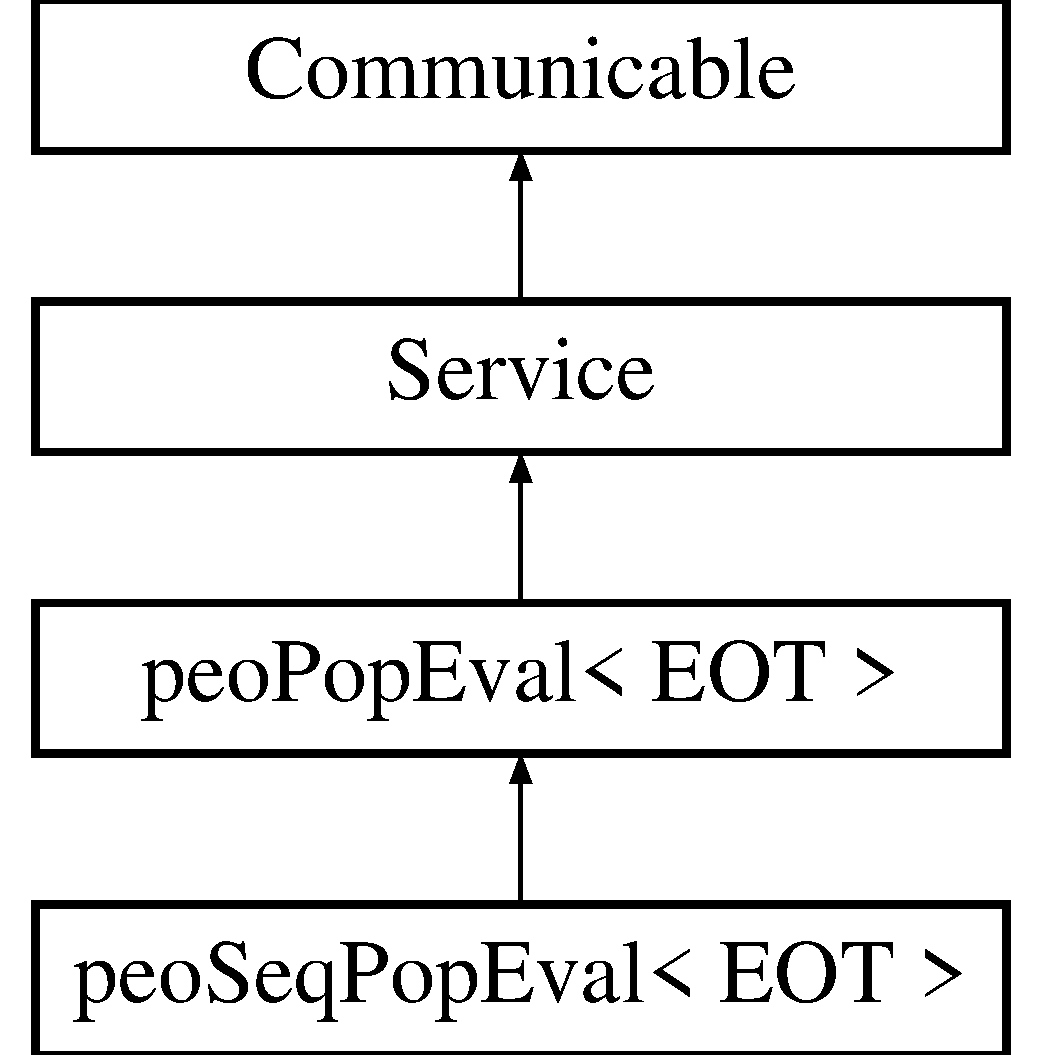
\includegraphics[height=4cm]{classpeoSeqPopEval}
\end{center}
\end{figure}
\subsection*{Public Member Functions}
\begin{CompactItemize}
\item 
\hyperlink{classpeoSeqPopEval_a41f91ab4b2aeb325ff75feb66d4e003}{peo\-Seq\-Pop\-Eval} (\bf{eo\-Eval\-Func}$<$ EOT $>$ \&\_\-\_\-eval)
\begin{CompactList}\small\item\em Constructor function - it only sets an internal reference to point to the specified evaluation object. \item\end{CompactList}\item 
void \hyperlink{classpeoSeqPopEval_b2c88b9a3ad9091949acf741844eb02f}{operator()} (\bf{eo\-Pop}$<$ EOT $>$ \&\_\-\_\-pop)
\begin{CompactList}\small\item\em Operator for evaluating all the individuals of a given population - in a sequential iterative manner. \item\end{CompactList}\end{CompactItemize}
\subsection*{Private Attributes}
\begin{CompactItemize}
\item 
\hypertarget{classpeoSeqPopEval_5465f31386c6b96bc8f7fb9393a28a2f}{
\bf{eo\-Eval\-Func}$<$ EOT $>$ \& \hyperlink{classpeoSeqPopEval_5465f31386c6b96bc8f7fb9393a28a2f}{eval}}
\label{classpeoSeqPopEval_5465f31386c6b96bc8f7fb9393a28a2f}

\end{CompactItemize}


\subsection{Detailed Description}
\subsubsection*{template$<$class EOT$>$ class peo\-Seq\-Pop\-Eval$<$ EOT $>$}

The \hyperlink{classpeoSeqPopEval}{peo\-Seq\-Pop\-Eval} class acts only as a Paradis\-EO specific sequential evaluation functor - a wrapper for incorporating an {\bf eo\-Eval\-Func$<$ EOT $>$}-derived class as evaluation functor. 

The specified \doxyref{EO} evaluation object is applyied in an iterative manner to each individual of a specified population. 



Definition at line 49 of file peo\-Seq\-Pop\-Eval.h.

\subsection{Constructor \& Destructor Documentation}
\hypertarget{classpeoSeqPopEval_a41f91ab4b2aeb325ff75feb66d4e003}{
\index{peoSeqPopEval@{peo\-Seq\-Pop\-Eval}!peoSeqPopEval@{peoSeqPopEval}}
\index{peoSeqPopEval@{peoSeqPopEval}!peoSeqPopEval@{peo\-Seq\-Pop\-Eval}}
\subsubsection[peoSeqPopEval]{\setlength{\rightskip}{0pt plus 5cm}template$<$class EOT$>$ \hyperlink{classpeoSeqPopEval}{peo\-Seq\-Pop\-Eval}$<$ EOT $>$::\hyperlink{classpeoSeqPopEval}{peo\-Seq\-Pop\-Eval} (\bf{eo\-Eval\-Func}$<$ EOT $>$ \& {\em \_\-\_\-eval})}}
\label{classpeoSeqPopEval_a41f91ab4b2aeb325ff75feb66d4e003}


Constructor function - it only sets an internal reference to point to the specified evaluation object. 

\begin{Desc}
\item[Parameters:]
\begin{description}
\item[{\em eo\-Eval\-Func$<$}]EOT $>$\& \_\-\_\-eval - evaluation object to be applied for each individual of a specified population \end{description}
\end{Desc}


Definition at line 69 of file peo\-Seq\-Pop\-Eval.h.

\subsection{Member Function Documentation}
\hypertarget{classpeoSeqPopEval_b2c88b9a3ad9091949acf741844eb02f}{
\index{peoSeqPopEval@{peo\-Seq\-Pop\-Eval}!operator()@{operator()}}
\index{operator()@{operator()}!peoSeqPopEval@{peo\-Seq\-Pop\-Eval}}
\subsubsection[operator()]{\setlength{\rightskip}{0pt plus 5cm}template$<$class EOT$>$ void \hyperlink{classpeoSeqPopEval}{peo\-Seq\-Pop\-Eval}$<$ EOT $>$::operator() (\bf{eo\-Pop}$<$ EOT $>$ \& {\em \_\-\_\-pop})\hspace{0.3cm}{\tt  \mbox{[}virtual\mbox{]}}}}
\label{classpeoSeqPopEval_b2c88b9a3ad9091949acf741844eb02f}


Operator for evaluating all the individuals of a given population - in a sequential iterative manner. 

\begin{Desc}
\item[Parameters:]
\begin{description}
\item[{\em eo\-Pop$<$}]EOT $>$\& \_\-\_\-pop - population to be evaluated. \end{description}
\end{Desc}


Implements \hyperlink{classpeoPopEval_2f208067a5e39c3b26c1234050a41e8f}{peo\-Pop\-Eval$<$ EOT $>$}.

Definition at line 74 of file peo\-Seq\-Pop\-Eval.h.

References peo\-Seq\-Pop\-Eval$<$ EOT $>$::eval.

The documentation for this class was generated from the following file:\begin{CompactItemize}
\item 
peo\-Seq\-Pop\-Eval.h\end{CompactItemize}

\hypertarget{classpeoSeqTransform}{
\section{peo\-Seq\-Transform$<$ EOT $>$ Class Template Reference}
\label{classpeoSeqTransform}\index{peoSeqTransform@{peoSeqTransform}}
}
The \hyperlink{classpeoSeqTransform}{peo\-Seq\-Transform} represent a wrapper for offering the possibility of using \doxyref{EO} derived transform operators along with the Paradis\-EO evolutionary algorithms.  


{\tt \#include $<$peo\-Seq\-Transform.h$>$}

Inheritance diagram for peo\-Seq\-Transform$<$ EOT $>$::\begin{figure}[H]
\begin{center}
\leavevmode
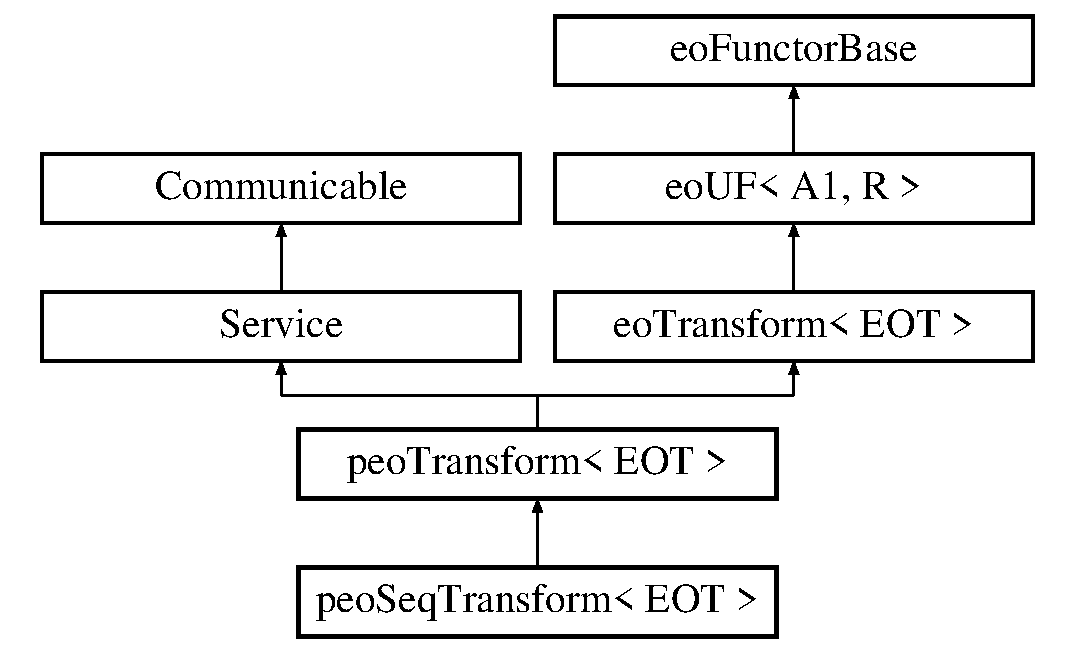
\includegraphics[height=5cm]{classpeoSeqTransform}
\end{center}
\end{figure}
\subsection*{Public Member Functions}
\begin{CompactItemize}
\item 
\hyperlink{classpeoSeqTransform_3b8e4ed19d9458938eb669d83a53c626}{peo\-Seq\-Transform} (\bf{eo\-Transform}$<$ EOT $>$ \&\_\-\_\-trans)
\begin{CompactList}\small\item\em Constructor function - sets an internal reference towards the specified EO-derived transform object. \item\end{CompactList}\item 
void \hyperlink{classpeoSeqTransform_1ba63536abb6c4e1c369e0b7e066872e}{operator()} (\bf{eo\-Pop}$<$ EOT $>$ \&\_\-\_\-pop)
\begin{CompactList}\small\item\em Operator for applying the specified transform operators on each individual of the given population. \item\end{CompactList}\item 
\hypertarget{classpeoSeqTransform_c4bf2724e9f6055f12bd169fad893be3}{
virtual void \hyperlink{classpeoSeqTransform_c4bf2724e9f6055f12bd169fad893be3}{pack\-Data} ()}
\label{classpeoSeqTransform_c4bf2724e9f6055f12bd169fad893be3}

\begin{CompactList}\small\item\em Interface function for providing a link with the parallel architecture of the Paradis\-EO framework. \item\end{CompactList}\item 
\hypertarget{classpeoSeqTransform_24e6cf15ef230ed538031b522ddd4ae6}{
virtual void \hyperlink{classpeoSeqTransform_24e6cf15ef230ed538031b522ddd4ae6}{unpack\-Data} ()}
\label{classpeoSeqTransform_24e6cf15ef230ed538031b522ddd4ae6}

\begin{CompactList}\small\item\em Interface function for providing a link with the parallel architecture of the Paradis\-EO framework. \item\end{CompactList}\item 
\hypertarget{classpeoSeqTransform_0294a2f9d6b44ec74d22eaceccdffc2b}{
virtual void \hyperlink{classpeoSeqTransform_0294a2f9d6b44ec74d22eaceccdffc2b}{execute} ()}
\label{classpeoSeqTransform_0294a2f9d6b44ec74d22eaceccdffc2b}

\begin{CompactList}\small\item\em Interface function for providing a link with the parallel architecture of the Paradis\-EO framework. \item\end{CompactList}\item 
\hypertarget{classpeoSeqTransform_4861c61f9e46d83964ea8a156a9a3ee0}{
virtual void \hyperlink{classpeoSeqTransform_4861c61f9e46d83964ea8a156a9a3ee0}{pack\-Result} ()}
\label{classpeoSeqTransform_4861c61f9e46d83964ea8a156a9a3ee0}

\begin{CompactList}\small\item\em Interface function for providing a link with the parallel architecture of the Paradis\-EO framework. \item\end{CompactList}\item 
\hypertarget{classpeoSeqTransform_5dd029fc011eb2a810ca1140025129b1}{
virtual void \hyperlink{classpeoSeqTransform_5dd029fc011eb2a810ca1140025129b1}{unpack\-Result} ()}
\label{classpeoSeqTransform_5dd029fc011eb2a810ca1140025129b1}

\begin{CompactList}\small\item\em Interface function for providing a link with the parallel architecture of the Paradis\-EO framework. \item\end{CompactList}\end{CompactItemize}
\subsection*{Private Attributes}
\begin{CompactItemize}
\item 
\hypertarget{classpeoSeqTransform_ad3e16c59dd6c46dfc1baf7b88af30cf}{
\bf{eo\-Transform}$<$ EOT $>$ \& \hyperlink{classpeoSeqTransform_ad3e16c59dd6c46dfc1baf7b88af30cf}{trans}}
\label{classpeoSeqTransform_ad3e16c59dd6c46dfc1baf7b88af30cf}

\end{CompactItemize}


\subsection{Detailed Description}
\subsubsection*{template$<$class EOT$>$ class peo\-Seq\-Transform$<$ EOT $>$}

The \hyperlink{classpeoSeqTransform}{peo\-Seq\-Transform} represent a wrapper for offering the possibility of using \doxyref{EO} derived transform operators along with the Paradis\-EO evolutionary algorithms. 

A minimal set of interface functions is also provided for creating the link with the parallel architecture of the Paradis\-EO framework. 



Definition at line 48 of file peo\-Seq\-Transform.h.

\subsection{Constructor \& Destructor Documentation}
\hypertarget{classpeoSeqTransform_3b8e4ed19d9458938eb669d83a53c626}{
\index{peoSeqTransform@{peo\-Seq\-Transform}!peoSeqTransform@{peoSeqTransform}}
\index{peoSeqTransform@{peoSeqTransform}!peoSeqTransform@{peo\-Seq\-Transform}}
\subsubsection[peoSeqTransform]{\setlength{\rightskip}{0pt plus 5cm}template$<$class EOT$>$ \hyperlink{classpeoSeqTransform}{peo\-Seq\-Transform}$<$ EOT $>$::\hyperlink{classpeoSeqTransform}{peo\-Seq\-Transform} (\bf{eo\-Transform}$<$ EOT $>$ \& {\em \_\-\_\-trans})}}
\label{classpeoSeqTransform_3b8e4ed19d9458938eb669d83a53c626}


Constructor function - sets an internal reference towards the specified EO-derived transform object. 

\begin{Desc}
\item[Parameters:]
\begin{description}
\item[{\em eo\-Transform$<$}]EOT $>$\& \_\-\_\-trans - EO-derived transform object including crossover and mutation operators. \end{description}
\end{Desc}


Definition at line 83 of file peo\-Seq\-Transform.h.

\subsection{Member Function Documentation}
\hypertarget{classpeoSeqTransform_1ba63536abb6c4e1c369e0b7e066872e}{
\index{peoSeqTransform@{peo\-Seq\-Transform}!operator()@{operator()}}
\index{operator()@{operator()}!peoSeqTransform@{peo\-Seq\-Transform}}
\subsubsection[operator()]{\setlength{\rightskip}{0pt plus 5cm}template$<$class EOT$>$ void \hyperlink{classpeoSeqTransform}{peo\-Seq\-Transform}$<$ EOT $>$::operator() (\bf{eo\-Pop}$<$ EOT $>$ \& {\em \_\-\_\-pop})}}
\label{classpeoSeqTransform_1ba63536abb6c4e1c369e0b7e066872e}


Operator for applying the specified transform operators on each individual of the given population. 

\begin{Desc}
\item[Parameters:]
\begin{description}
\item[{\em eo\-Pop$<$}]EOT $>$\& \_\-\_\-pop - population to be transformed by applying the crossover and mutation operators. \end{description}
\end{Desc}


Definition at line 88 of file peo\-Seq\-Transform.h.

References peo\-Seq\-Transform$<$ EOT $>$::trans.

The documentation for this class was generated from the following file:\begin{CompactItemize}
\item 
peo\-Seq\-Transform.h\end{CompactItemize}

\hypertarget{classpeoSynchronousMultiStart}{
\section{peo\-Synchronous\-Multi\-Start$<$ Entity\-Type $>$ Class Template Reference}
\label{classpeoSynchronousMultiStart}\index{peoSynchronousMultiStart@{peoSynchronousMultiStart}}
}
Inheritance diagram for peo\-Synchronous\-Multi\-Start$<$ Entity\-Type $>$::\begin{figure}[H]
\begin{center}
\leavevmode
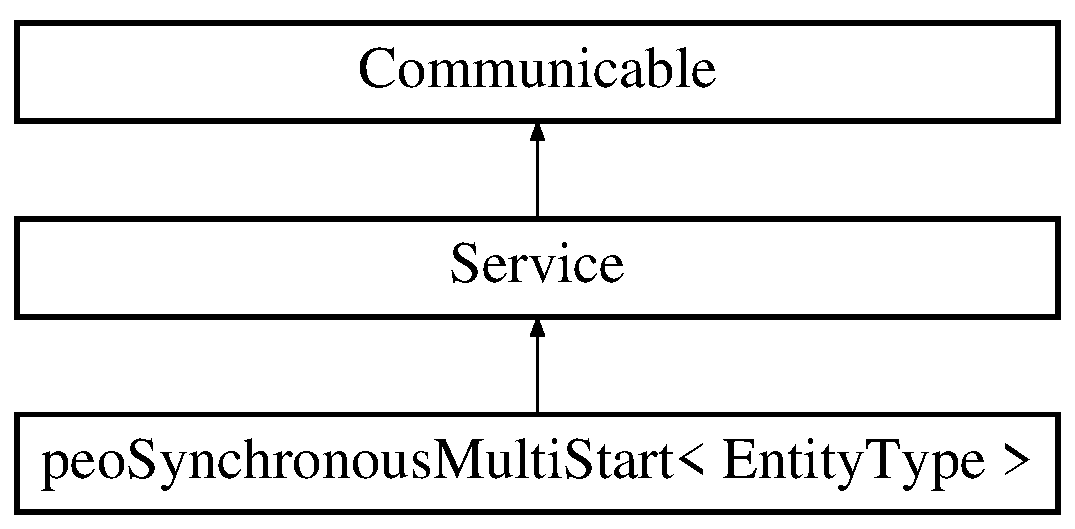
\includegraphics[height=3cm]{classpeoSynchronousMultiStart}
\end{center}
\end{figure}
\subsection*{Public Member Functions}
\begin{CompactItemize}
\item 
\hypertarget{classpeoSynchronousMultiStart_e9a336c61dd6216d7d15253ff9c9d2a3}{
template$<$typename Algorithm\-Type$>$ \hyperlink{classpeoSynchronousMultiStart_e9a336c61dd6216d7d15253ff9c9d2a3}{peo\-Synchronous\-Multi\-Start} (Algorithm\-Type \&external\-Algorithm)}
\label{classpeoSynchronousMultiStart_e9a336c61dd6216d7d15253ff9c9d2a3}

\item 
\hypertarget{classpeoSynchronousMultiStart_689374232ff67f266ddaa5d309ea54ac}{
template$<$typename Algorithm\-Type, typename Aggregation\-Function\-Type$>$ \hyperlink{classpeoSynchronousMultiStart_689374232ff67f266ddaa5d309ea54ac}{peo\-Synchronous\-Multi\-Start} (std::vector$<$ Algorithm\-Type $\ast$ $>$ \&external\-Algorithms, Aggregation\-Function\-Type \&external\-Aggregation\-Function)}
\label{classpeoSynchronousMultiStart_689374232ff67f266ddaa5d309ea54ac}

\item 
\hypertarget{classpeoSynchronousMultiStart_f9ec55d67f5f45f5a737064fae569277}{
\hyperlink{classpeoSynchronousMultiStart_f9ec55d67f5f45f5a737064fae569277}{$\sim$peo\-Synchronous\-Multi\-Start} ()}
\label{classpeoSynchronousMultiStart_f9ec55d67f5f45f5a737064fae569277}

\item 
\hypertarget{classpeoSynchronousMultiStart_1fd09337a6edcf173edff1fdda2387c7}{
template$<$typename Type$>$ void \hyperlink{classpeoSynchronousMultiStart_1fd09337a6edcf173edff1fdda2387c7}{operator()} (Type \&external\-Data)}
\label{classpeoSynchronousMultiStart_1fd09337a6edcf173edff1fdda2387c7}

\item 
\hypertarget{classpeoSynchronousMultiStart_45372c26ac5b979d29458815debceff8}{
template$<$typename Type$>$ void \hyperlink{classpeoSynchronousMultiStart_45372c26ac5b979d29458815debceff8}{operator()} (const Type \&external\-Data\-Begin, const Type \&external\-Data\-End)}
\label{classpeoSynchronousMultiStart_45372c26ac5b979d29458815debceff8}

\item 
\hypertarget{classpeoSynchronousMultiStart_c73358b4f04f258c55f631660a7992fb}{
void \hyperlink{classpeoSynchronousMultiStart_c73358b4f04f258c55f631660a7992fb}{pack\-Data} ()}
\label{classpeoSynchronousMultiStart_c73358b4f04f258c55f631660a7992fb}

\item 
\hypertarget{classpeoSynchronousMultiStart_9881b3f05c9f90bcb3c3ec0af8109ccc}{
void \hyperlink{classpeoSynchronousMultiStart_9881b3f05c9f90bcb3c3ec0af8109ccc}{unpack\-Data} ()}
\label{classpeoSynchronousMultiStart_9881b3f05c9f90bcb3c3ec0af8109ccc}

\item 
\hypertarget{classpeoSynchronousMultiStart_da98ee86056eca293b3f08c89584b701}{
void \hyperlink{classpeoSynchronousMultiStart_da98ee86056eca293b3f08c89584b701}{execute} ()}
\label{classpeoSynchronousMultiStart_da98ee86056eca293b3f08c89584b701}

\item 
\hypertarget{classpeoSynchronousMultiStart_0a5e0e1c1db5af61351e201e019f5a89}{
void \hyperlink{classpeoSynchronousMultiStart_0a5e0e1c1db5af61351e201e019f5a89}{pack\-Result} ()}
\label{classpeoSynchronousMultiStart_0a5e0e1c1db5af61351e201e019f5a89}

\item 
\hypertarget{classpeoSynchronousMultiStart_976b78c11073ee3be09c1aed7826411a}{
void \hyperlink{classpeoSynchronousMultiStart_976b78c11073ee3be09c1aed7826411a}{unpack\-Result} ()}
\label{classpeoSynchronousMultiStart_976b78c11073ee3be09c1aed7826411a}

\item 
\hypertarget{classpeoSynchronousMultiStart_de581c634fa9f952d571f9ed0a6611ed}{
void \hyperlink{classpeoSynchronousMultiStart_de581c634fa9f952d571f9ed0a6611ed}{notify\-Sending\-Data} ()}
\label{classpeoSynchronousMultiStart_de581c634fa9f952d571f9ed0a6611ed}

\item 
\hypertarget{classpeoSynchronousMultiStart_e328547d97849bfc85f2a7356e5e7927}{
void \hyperlink{classpeoSynchronousMultiStart_e328547d97849bfc85f2a7356e5e7927}{notify\-Sending\-All\-Resource\-Requests} ()}
\label{classpeoSynchronousMultiStart_e328547d97849bfc85f2a7356e5e7927}

\end{CompactItemize}
\subsection*{Private Attributes}
\begin{CompactItemize}
\item 
\hypertarget{classpeoSynchronousMultiStart_ea22b8cd0f4974da519ec416904d772e}{
\hyperlink{structpeoSynchronousMultiStart_1_1AbstractAlgorithm}{Abstract\-Algorithm} $\ast$ \hyperlink{classpeoSynchronousMultiStart_ea22b8cd0f4974da519ec416904d772e}{singular\-Algorithm}}
\label{classpeoSynchronousMultiStart_ea22b8cd0f4974da519ec416904d772e}

\item 
\hypertarget{classpeoSynchronousMultiStart_f47bb795f53df73f04c0d1528fa346a6}{
std::vector$<$ \hyperlink{structpeoSynchronousMultiStart_1_1AbstractAlgorithm}{Abstract\-Algorithm} $\ast$ $>$ \hyperlink{classpeoSynchronousMultiStart_f47bb795f53df73f04c0d1528fa346a6}{algorithms}}
\label{classpeoSynchronousMultiStart_f47bb795f53df73f04c0d1528fa346a6}

\item 
\hypertarget{classpeoSynchronousMultiStart_abcd58d71eabf2fab35c662fb300e61c}{
\hyperlink{structpeoSynchronousMultiStart_1_1AbstractAggregationAlgorithm}{Abstract\-Aggregation\-Algorithm} $\ast$ \hyperlink{classpeoSynchronousMultiStart_abcd58d71eabf2fab35c662fb300e61c}{aggregation\-Function}}
\label{classpeoSynchronousMultiStart_abcd58d71eabf2fab35c662fb300e61c}

\item 
\hypertarget{classpeoSynchronousMultiStart_6efedfa64f7a4f3a0d81002e8226dcea}{
Entity\-Type \hyperlink{classpeoSynchronousMultiStart_6efedfa64f7a4f3a0d81002e8226dcea}{entity\-Type\-Instance}}
\label{classpeoSynchronousMultiStart_6efedfa64f7a4f3a0d81002e8226dcea}

\item 
\hypertarget{classpeoSynchronousMultiStart_f729f5a1671437dce7607ad5b7253560}{
std::vector$<$ \hyperlink{structpeoSynchronousMultiStart_1_1AbstractDataType}{Abstract\-Data\-Type} $\ast$ $>$ \hyperlink{classpeoSynchronousMultiStart_f729f5a1671437dce7607ad5b7253560}{data}}
\label{classpeoSynchronousMultiStart_f729f5a1671437dce7607ad5b7253560}

\item 
\hypertarget{classpeoSynchronousMultiStart_0264a28725fb4a030ed1e4010e07e69e}{
unsigned \hyperlink{classpeoSynchronousMultiStart_0264a28725fb4a030ed1e4010e07e69e}{idx}}
\label{classpeoSynchronousMultiStart_0264a28725fb4a030ed1e4010e07e69e}

\item 
\hypertarget{classpeoSynchronousMultiStart_e8c889e6228535ce02086c76d3480cbb}{
unsigned \hyperlink{classpeoSynchronousMultiStart_e8c889e6228535ce02086c76d3480cbb}{num\_\-term}}
\label{classpeoSynchronousMultiStart_e8c889e6228535ce02086c76d3480cbb}

\item 
\hypertarget{classpeoSynchronousMultiStart_a49cb2d76e6fdbfdbe0788c8388d6a0f}{
unsigned \hyperlink{classpeoSynchronousMultiStart_a49cb2d76e6fdbfdbe0788c8388d6a0f}{data\-Index}}
\label{classpeoSynchronousMultiStart_a49cb2d76e6fdbfdbe0788c8388d6a0f}

\item 
\hypertarget{classpeoSynchronousMultiStart_20cff9a01fb7bb621264b901dab7f336}{
unsigned \hyperlink{classpeoSynchronousMultiStart_20cff9a01fb7bb621264b901dab7f336}{function\-Index}}
\label{classpeoSynchronousMultiStart_20cff9a01fb7bb621264b901dab7f336}

\end{CompactItemize}
\subsection*{Classes}
\begin{CompactItemize}
\item 
struct \hyperlink{structpeoSynchronousMultiStart_1_1AbstractAggregationAlgorithm}{Abstract\-Aggregation\-Algorithm}
\item 
struct \hyperlink{structpeoSynchronousMultiStart_1_1AbstractAlgorithm}{Abstract\-Algorithm}
\item 
struct \hyperlink{structpeoSynchronousMultiStart_1_1AbstractDataType}{Abstract\-Data\-Type}
\item 
struct \hyperlink{structpeoSynchronousMultiStart_1_1AggregationAlgorithm}{Aggregation\-Algorithm}
\item 
struct \hyperlink{structpeoSynchronousMultiStart_1_1Algorithm}{Algorithm}
\item 
struct \hyperlink{structpeoSynchronousMultiStart_1_1DataType}{Data\-Type}
\item 
struct \hyperlink{structpeoSynchronousMultiStart_1_1NoAggregationFunction}{No\-Aggregation\-Function}
\end{CompactItemize}


\subsection{Detailed Description}
\subsubsection*{template$<$typename Entity\-Type$>$ class peo\-Synchronous\-Multi\-Start$<$ Entity\-Type $>$}





Definition at line 45 of file peo\-Synchronous\-Multi\-Start.h.

The documentation for this class was generated from the following file:\begin{CompactItemize}
\item 
peo\-Synchronous\-Multi\-Start.h\end{CompactItemize}

\hypertarget{structpeoSynchronousMultiStart_1_1AbstractAggregationAlgorithm}{
\section{peo\-Synchronous\-Multi\-Start$<$ Entity\-Type $>$::Abstract\-Aggregation\-Algorithm Struct Reference}
\label{structpeoSynchronousMultiStart_1_1AbstractAggregationAlgorithm}\index{peoSynchronousMultiStart::AbstractAggregationAlgorithm@{peoSynchronousMultiStart::AbstractAggregationAlgorithm}}
}
Inheritance diagram for peo\-Synchronous\-Multi\-Start$<$ Entity\-Type $>$::Abstract\-Aggregation\-Algorithm::\begin{figure}[H]
\begin{center}
\leavevmode
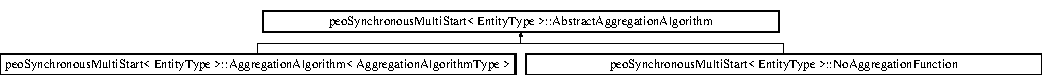
\includegraphics[height=1.01083cm]{structpeoSynchronousMultiStart_1_1AbstractAggregationAlgorithm}
\end{center}
\end{figure}
\subsection*{Public Member Functions}
\begin{CompactItemize}
\item 
\hypertarget{structpeoSynchronousMultiStart_1_1AbstractAggregationAlgorithm_d5bb9f3712564b788bb7c6da71ef2d3f}{
virtual \hyperlink{structpeoSynchronousMultiStart_1_1AbstractAggregationAlgorithm_d5bb9f3712564b788bb7c6da71ef2d3f}{$\sim$Abstract\-Aggregation\-Algorithm} ()}
\label{structpeoSynchronousMultiStart_1_1AbstractAggregationAlgorithm_d5bb9f3712564b788bb7c6da71ef2d3f}

\item 
\hypertarget{structpeoSynchronousMultiStart_1_1AbstractAggregationAlgorithm_cf9b3275e26f24984c9bb839e7f07ba6}{
virtual void \hyperlink{structpeoSynchronousMultiStart_1_1AbstractAggregationAlgorithm_cf9b3275e26f24984c9bb839e7f07ba6}{operator()} (\hyperlink{structpeoSynchronousMultiStart_1_1AbstractDataType}{Abstract\-Data\-Type} \&data\-Type\-Instance\-A, \hyperlink{structpeoSynchronousMultiStart_1_1AbstractDataType}{Abstract\-Data\-Type} \&data\-Type\-Instance\-B)}
\label{structpeoSynchronousMultiStart_1_1AbstractAggregationAlgorithm_cf9b3275e26f24984c9bb839e7f07ba6}

\end{CompactItemize}


\subsection{Detailed Description}
\subsubsection*{template$<$typename Entity\-Type$>$ struct peo\-Synchronous\-Multi\-Start$<$ Entity\-Type $>$::Abstract\-Aggregation\-Algorithm}





Definition at line 157 of file peo\-Synchronous\-Multi\-Start.h.

The documentation for this struct was generated from the following file:\begin{CompactItemize}
\item 
peo\-Synchronous\-Multi\-Start.h\end{CompactItemize}

\hypertarget{structpeoSynchronousMultiStart_1_1AbstractAlgorithm}{
\section{peo\-Synchronous\-Multi\-Start$<$ Entity\-Type $>$::Abstract\-Algorithm Struct Reference}
\label{structpeoSynchronousMultiStart_1_1AbstractAlgorithm}\index{peoSynchronousMultiStart::AbstractAlgorithm@{peoSynchronousMultiStart::AbstractAlgorithm}}
}
Inheritance diagram for peo\-Synchronous\-Multi\-Start$<$ Entity\-Type $>$::Abstract\-Algorithm::\begin{figure}[H]
\begin{center}
\leavevmode
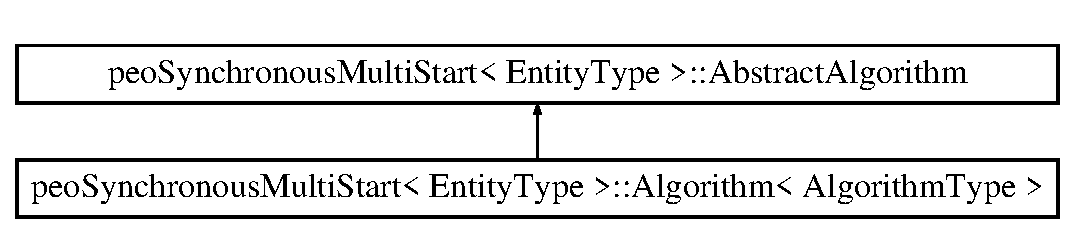
\includegraphics[height=2cm]{structpeoSynchronousMultiStart_1_1AbstractAlgorithm}
\end{center}
\end{figure}
\subsection*{Public Member Functions}
\begin{CompactItemize}
\item 
\hypertarget{structpeoSynchronousMultiStart_1_1AbstractAlgorithm_c77be114590c79c1b96d3afbe73596e0}{
virtual \hyperlink{structpeoSynchronousMultiStart_1_1AbstractAlgorithm_c77be114590c79c1b96d3afbe73596e0}{$\sim$Abstract\-Algorithm} ()}
\label{structpeoSynchronousMultiStart_1_1AbstractAlgorithm_c77be114590c79c1b96d3afbe73596e0}

\item 
\hypertarget{structpeoSynchronousMultiStart_1_1AbstractAlgorithm_a5f7790ac2b99e798e4e84f2d5a5f78c}{
virtual void \hyperlink{structpeoSynchronousMultiStart_1_1AbstractAlgorithm_a5f7790ac2b99e798e4e84f2d5a5f78c}{operator()} (\hyperlink{structpeoSynchronousMultiStart_1_1AbstractDataType}{Abstract\-Data\-Type} \&data\-Type\-Instance)}
\label{structpeoSynchronousMultiStart_1_1AbstractAlgorithm_a5f7790ac2b99e798e4e84f2d5a5f78c}

\end{CompactItemize}


\subsection{Detailed Description}
\subsubsection*{template$<$typename Entity\-Type$>$ struct peo\-Synchronous\-Multi\-Start$<$ Entity\-Type $>$::Abstract\-Algorithm}





Definition at line 139 of file peo\-Synchronous\-Multi\-Start.h.

The documentation for this struct was generated from the following file:\begin{CompactItemize}
\item 
peo\-Synchronous\-Multi\-Start.h\end{CompactItemize}

\hypertarget{structpeoSynchronousMultiStart_1_1AbstractDataType}{
\section{peo\-Synchronous\-Multi\-Start$<$ Entity\-Type $>$::Abstract\-Data\-Type Struct Reference}
\label{structpeoSynchronousMultiStart_1_1AbstractDataType}\index{peoSynchronousMultiStart::AbstractDataType@{peoSynchronousMultiStart::AbstractDataType}}
}
Inheritance diagram for peo\-Synchronous\-Multi\-Start$<$ Entity\-Type $>$::Abstract\-Data\-Type::\begin{figure}[H]
\begin{center}
\leavevmode
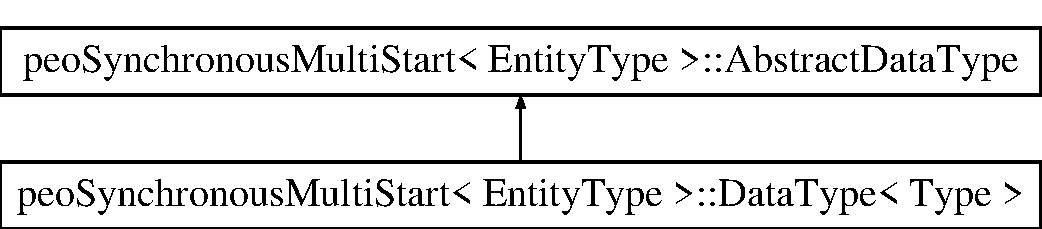
\includegraphics[height=2cm]{structpeoSynchronousMultiStart_1_1AbstractDataType}
\end{center}
\end{figure}
\subsection*{Public Member Functions}
\begin{CompactItemize}
\item 
\hypertarget{structpeoSynchronousMultiStart_1_1AbstractDataType_4d868a93f8e97621ec5c7b6a2e28b265}{
virtual \hyperlink{structpeoSynchronousMultiStart_1_1AbstractDataType_4d868a93f8e97621ec5c7b6a2e28b265}{$\sim$Abstract\-Data\-Type} ()}
\label{structpeoSynchronousMultiStart_1_1AbstractDataType_4d868a93f8e97621ec5c7b6a2e28b265}

\item 
\hypertarget{structpeoSynchronousMultiStart_1_1AbstractDataType_a4addfca8a9acecadb4c786deed36934}{
template$<$typename Type$>$ \hyperlink{structpeoSynchronousMultiStart_1_1AbstractDataType_a4addfca8a9acecadb4c786deed36934}{operator Type \&} ()}
\label{structpeoSynchronousMultiStart_1_1AbstractDataType_a4addfca8a9acecadb4c786deed36934}

\end{CompactItemize}


\subsection{Detailed Description}
\subsubsection*{template$<$typename Entity\-Type$>$ struct peo\-Synchronous\-Multi\-Start$<$ Entity\-Type $>$::Abstract\-Data\-Type}





Definition at line 122 of file peo\-Synchronous\-Multi\-Start.h.

The documentation for this struct was generated from the following file:\begin{CompactItemize}
\item 
peo\-Synchronous\-Multi\-Start.h\end{CompactItemize}

\hypertarget{structpeoSynchronousMultiStart_1_1AggregationAlgorithm}{
\section{peo\-Synchronous\-Multi\-Start$<$ Entity\-Type $>$::Aggregation\-Algorithm$<$ Aggregation\-Algorithm\-Type $>$ Struct Template Reference}
\label{structpeoSynchronousMultiStart_1_1AggregationAlgorithm}\index{peoSynchronousMultiStart::AggregationAlgorithm@{peoSynchronousMultiStart::AggregationAlgorithm}}
}
Inheritance diagram for peo\-Synchronous\-Multi\-Start$<$ Entity\-Type $>$::Aggregation\-Algorithm$<$ Aggregation\-Algorithm\-Type $>$::\begin{figure}[H]
\begin{center}
\leavevmode
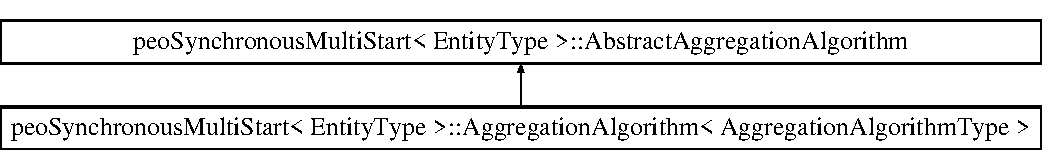
\includegraphics[height=2cm]{structpeoSynchronousMultiStart_1_1AggregationAlgorithm}
\end{center}
\end{figure}
\subsection*{Public Member Functions}
\begin{CompactItemize}
\item 
\hypertarget{structpeoSynchronousMultiStart_1_1AggregationAlgorithm_1e03bf7728d19f4649366238962ca365}{
\hyperlink{structpeoSynchronousMultiStart_1_1AggregationAlgorithm_1e03bf7728d19f4649366238962ca365}{Aggregation\-Algorithm} (Aggregation\-Algorithm\-Type \&external\-Aggregation\-Algorithm)}
\label{structpeoSynchronousMultiStart_1_1AggregationAlgorithm_1e03bf7728d19f4649366238962ca365}

\item 
\hypertarget{structpeoSynchronousMultiStart_1_1AggregationAlgorithm_f8abe94db942aa42f0e3d9c1657db581}{
void \hyperlink{structpeoSynchronousMultiStart_1_1AggregationAlgorithm_f8abe94db942aa42f0e3d9c1657db581}{operator()} (\hyperlink{structpeoSynchronousMultiStart_1_1AbstractDataType}{Abstract\-Data\-Type} \&data\-Type\-Instance\-A, \hyperlink{structpeoSynchronousMultiStart_1_1AbstractDataType}{Abstract\-Data\-Type} \&data\-Type\-Instance\-B)}
\label{structpeoSynchronousMultiStart_1_1AggregationAlgorithm_f8abe94db942aa42f0e3d9c1657db581}

\end{CompactItemize}
\subsection*{Public Attributes}
\begin{CompactItemize}
\item 
\hypertarget{structpeoSynchronousMultiStart_1_1AggregationAlgorithm_3c701a64f21aa00278c58b5b4ac914a1}{
Aggregation\-Algorithm\-Type \& \hyperlink{structpeoSynchronousMultiStart_1_1AggregationAlgorithm_3c701a64f21aa00278c58b5b4ac914a1}{aggregation\-Algorithm}}
\label{structpeoSynchronousMultiStart_1_1AggregationAlgorithm_3c701a64f21aa00278c58b5b4ac914a1}

\end{CompactItemize}


\subsection{Detailed Description}
\subsubsection*{template$<$typename Entity\-Type$>$template$<$typename Aggregation\-Algorithm\-Type$>$ struct peo\-Synchronous\-Multi\-Start$<$ Entity\-Type $>$::Aggregation\-Algorithm$<$ Aggregation\-Algorithm\-Type $>$}





Definition at line 164 of file peo\-Synchronous\-Multi\-Start.h.

The documentation for this struct was generated from the following file:\begin{CompactItemize}
\item 
peo\-Synchronous\-Multi\-Start.h\end{CompactItemize}

\hypertarget{structpeoSynchronousMultiStart_1_1Algorithm}{
\section{peo\-Synchronous\-Multi\-Start$<$ Entity\-Type $>$::Algorithm$<$ Algorithm\-Type $>$ Struct Template Reference}
\label{structpeoSynchronousMultiStart_1_1Algorithm}\index{peoSynchronousMultiStart::Algorithm@{peoSynchronousMultiStart::Algorithm}}
}
Inheritance diagram for peo\-Synchronous\-Multi\-Start$<$ Entity\-Type $>$::Algorithm$<$ Algorithm\-Type $>$::\begin{figure}[H]
\begin{center}
\leavevmode
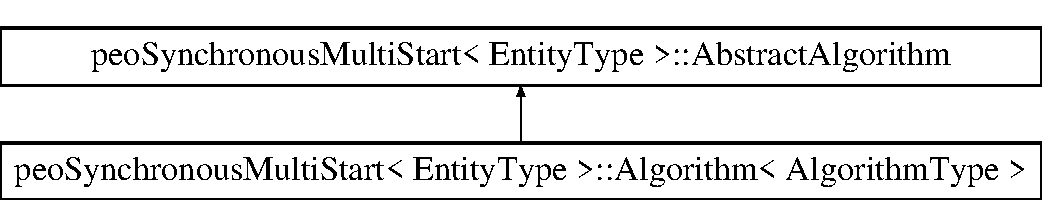
\includegraphics[height=2cm]{structpeoSynchronousMultiStart_1_1Algorithm}
\end{center}
\end{figure}
\subsection*{Public Member Functions}
\begin{CompactItemize}
\item 
\hypertarget{structpeoSynchronousMultiStart_1_1Algorithm_8ba4ac2674ca61a8e6b0af2e8e25ba66}{
\hyperlink{structpeoSynchronousMultiStart_1_1Algorithm_8ba4ac2674ca61a8e6b0af2e8e25ba66}{Algorithm} (Algorithm\-Type \&external\-Algorithm)}
\label{structpeoSynchronousMultiStart_1_1Algorithm_8ba4ac2674ca61a8e6b0af2e8e25ba66}

\item 
\hypertarget{structpeoSynchronousMultiStart_1_1Algorithm_d8902e501b61a8d5727589a5a106bb10}{
void \hyperlink{structpeoSynchronousMultiStart_1_1Algorithm_d8902e501b61a8d5727589a5a106bb10}{operator()} (\hyperlink{structpeoSynchronousMultiStart_1_1AbstractDataType}{Abstract\-Data\-Type} \&data\-Type\-Instance)}
\label{structpeoSynchronousMultiStart_1_1Algorithm_d8902e501b61a8d5727589a5a106bb10}

\end{CompactItemize}
\subsection*{Public Attributes}
\begin{CompactItemize}
\item 
\hypertarget{structpeoSynchronousMultiStart_1_1Algorithm_2d533c96d2eefea51a72d241d39abf22}{
Algorithm\-Type \& \hyperlink{structpeoSynchronousMultiStart_1_1Algorithm_2d533c96d2eefea51a72d241d39abf22}{algorithm}}
\label{structpeoSynchronousMultiStart_1_1Algorithm_2d533c96d2eefea51a72d241d39abf22}

\end{CompactItemize}


\subsection{Detailed Description}
\subsubsection*{template$<$typename Entity\-Type$>$template$<$typename Algorithm\-Type$>$ struct peo\-Synchronous\-Multi\-Start$<$ Entity\-Type $>$::Algorithm$<$ Algorithm\-Type $>$}





Definition at line 146 of file peo\-Synchronous\-Multi\-Start.h.

The documentation for this struct was generated from the following file:\begin{CompactItemize}
\item 
peo\-Synchronous\-Multi\-Start.h\end{CompactItemize}

\hypertarget{structpeoSynchronousMultiStart_1_1DataType}{
\section{peo\-Synchronous\-Multi\-Start$<$ Entity\-Type $>$::Data\-Type$<$ Type $>$ Struct Template Reference}
\label{structpeoSynchronousMultiStart_1_1DataType}\index{peoSynchronousMultiStart::DataType@{peoSynchronousMultiStart::DataType}}
}
Inheritance diagram for peo\-Synchronous\-Multi\-Start$<$ Entity\-Type $>$::Data\-Type$<$ Type $>$::\begin{figure}[H]
\begin{center}
\leavevmode
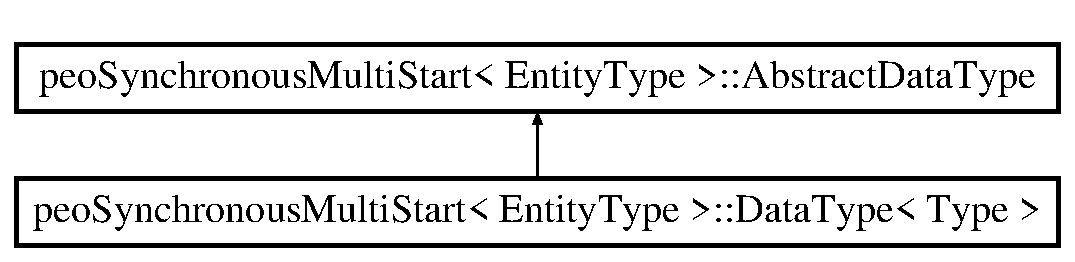
\includegraphics[height=2cm]{structpeoSynchronousMultiStart_1_1DataType}
\end{center}
\end{figure}
\subsection*{Public Member Functions}
\begin{CompactItemize}
\item 
\hypertarget{structpeoSynchronousMultiStart_1_1DataType_cf5b9add5416139738e152b461008a89}{
\hyperlink{structpeoSynchronousMultiStart_1_1DataType_cf5b9add5416139738e152b461008a89}{Data\-Type} (Type \&external\-Data)}
\label{structpeoSynchronousMultiStart_1_1DataType_cf5b9add5416139738e152b461008a89}

\end{CompactItemize}
\subsection*{Public Attributes}
\begin{CompactItemize}
\item 
\hypertarget{structpeoSynchronousMultiStart_1_1DataType_76abc322ae058a820b2c964907bc0d80}{
Type \& \hyperlink{structpeoSynchronousMultiStart_1_1DataType_76abc322ae058a820b2c964907bc0d80}{data}}
\label{structpeoSynchronousMultiStart_1_1DataType_76abc322ae058a820b2c964907bc0d80}

\end{CompactItemize}


\subsection{Detailed Description}
\subsubsection*{template$<$typename Entity\-Type$>$template$<$typename Type$>$ struct peo\-Synchronous\-Multi\-Start$<$ Entity\-Type $>$::Data\-Type$<$ Type $>$}





Definition at line 132 of file peo\-Synchronous\-Multi\-Start.h.

The documentation for this struct was generated from the following file:\begin{CompactItemize}
\item 
peo\-Synchronous\-Multi\-Start.h\end{CompactItemize}

\hypertarget{structpeoSynchronousMultiStart_1_1NoAggregationFunction}{
\section{peo\-Synchronous\-Multi\-Start$<$ Entity\-Type $>$::No\-Aggregation\-Function Struct Reference}
\label{structpeoSynchronousMultiStart_1_1NoAggregationFunction}\index{peoSynchronousMultiStart::NoAggregationFunction@{peoSynchronousMultiStart::NoAggregationFunction}}
}
Inheritance diagram for peo\-Synchronous\-Multi\-Start$<$ Entity\-Type $>$::No\-Aggregation\-Function::\begin{figure}[H]
\begin{center}
\leavevmode
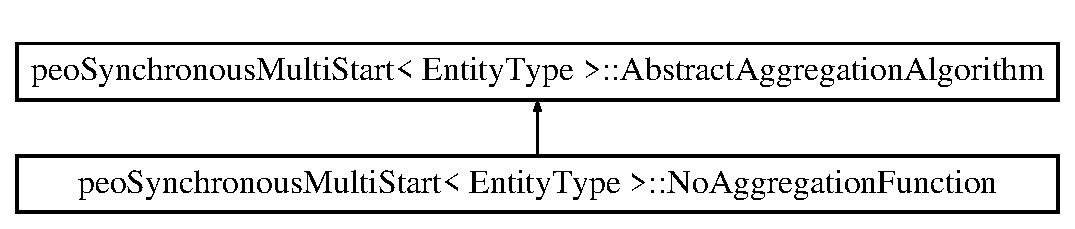
\includegraphics[height=2cm]{structpeoSynchronousMultiStart_1_1NoAggregationFunction}
\end{center}
\end{figure}
\subsection*{Public Member Functions}
\begin{CompactItemize}
\item 
\hypertarget{structpeoSynchronousMultiStart_1_1NoAggregationFunction_d094bb3cca92a48de0afadf576cda044}{
void \hyperlink{structpeoSynchronousMultiStart_1_1NoAggregationFunction_d094bb3cca92a48de0afadf576cda044}{operator()} (\hyperlink{structpeoSynchronousMultiStart_1_1AbstractDataType}{Abstract\-Data\-Type} \&data\-Type\-Instance\-A, \hyperlink{structpeoSynchronousMultiStart_1_1AbstractDataType}{Abstract\-Data\-Type} \&data\-Type\-Instance\-B)}
\label{structpeoSynchronousMultiStart_1_1NoAggregationFunction_d094bb3cca92a48de0afadf576cda044}

\end{CompactItemize}


\subsection{Detailed Description}
\subsubsection*{template$<$typename Entity\-Type$>$ struct peo\-Synchronous\-Multi\-Start$<$ Entity\-Type $>$::No\-Aggregation\-Function}





Definition at line 176 of file peo\-Synchronous\-Multi\-Start.h.

The documentation for this struct was generated from the following file:\begin{CompactItemize}
\item 
peo\-Synchronous\-Multi\-Start.h\end{CompactItemize}

\hypertarget{classpeoSyncIslandMig}{
\section{peo\-Sync\-Island\-Mig$<$ TYPESELECT, TYPEREPLACE $>$ Class Template Reference}
\label{classpeoSyncIslandMig}\index{peoSyncIslandMig@{peoSyncIslandMig}}
}
Specific class for a synchronous migration.  


{\tt \#include $<$peo\-Sync\-Island\-Mig.h$>$}

Inheritance diagram for peo\-Sync\-Island\-Mig$<$ TYPESELECT, TYPEREPLACE $>$::\begin{figure}[H]
\begin{center}
\leavevmode
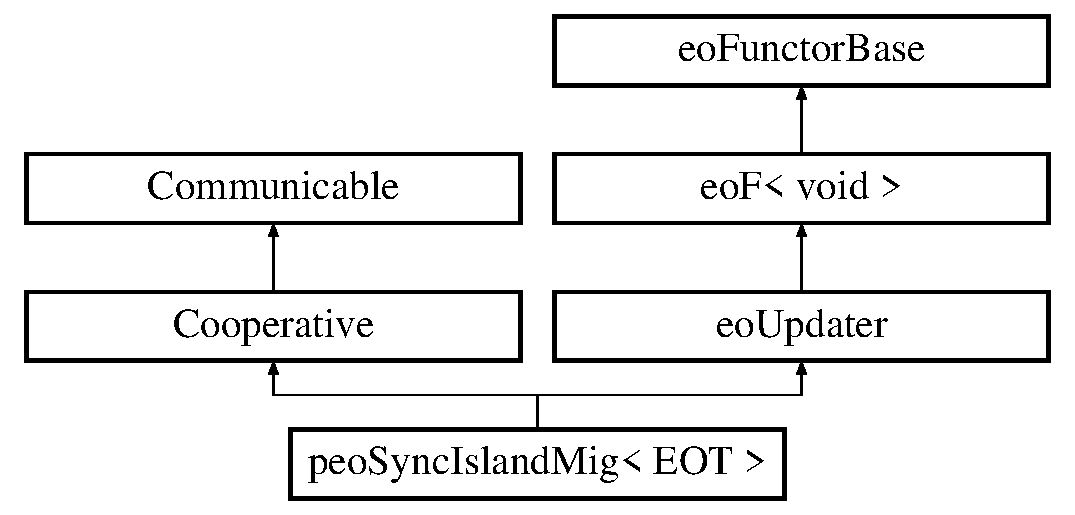
\includegraphics[height=3cm]{classpeoSyncIslandMig}
\end{center}
\end{figure}
\subsection*{Public Member Functions}
\begin{CompactItemize}
\item 
\hyperlink{classpeoSyncIslandMig_24f4d1ea8bb63c09b9d6cd8476014082}{peo\-Sync\-Island\-Mig} (unsigned \_\-\_\-frequency, \hyperlink{classselector}{selector}$<$ TYPESELECT $>$ \&\_\-\_\-select, \hyperlink{classreplacement}{replacement}$<$ TYPEREPLACE $>$ \&\_\-\_\-replace, \hyperlink{classTopology}{Topology} \&\_\-\_\-topology)
\item 
\hypertarget{classpeoSyncIslandMig_0fd5b3b4e467ee33ae0186c0ae9d58ef}{
void \hyperlink{classpeoSyncIslandMig_0fd5b3b4e467ee33ae0186c0ae9d58ef}{operator()} ()}
\label{classpeoSyncIslandMig_0fd5b3b4e467ee33ae0186c0ae9d58ef}

\begin{CompactList}\small\item\em operator \item\end{CompactList}\item 
\hypertarget{classpeoSyncIslandMig_2daadf9928b8075ea469ca3cc49ddc88}{
void \hyperlink{classpeoSyncIslandMig_2daadf9928b8075ea469ca3cc49ddc88}{pack} ()}
\label{classpeoSyncIslandMig_2daadf9928b8075ea469ca3cc49ddc88}

\begin{CompactList}\small\item\em Function realizing packages. \item\end{CompactList}\item 
\hypertarget{classpeoSyncIslandMig_25bc1a03cc49e17dda34b6647df1f9c5}{
void \hyperlink{classpeoSyncIslandMig_25bc1a03cc49e17dda34b6647df1f9c5}{unpack} ()}
\label{classpeoSyncIslandMig_25bc1a03cc49e17dda34b6647df1f9c5}

\begin{CompactList}\small\item\em Function reconstituting packages. \item\end{CompactList}\item 
\hypertarget{classpeoSyncIslandMig_956f56110bccff8c8fae4b05aa804d32}{
void \hyperlink{classpeoSyncIslandMig_956f56110bccff8c8fae4b05aa804d32}{pack\-Synchronize\-Req} ()}
\label{classpeoSyncIslandMig_956f56110bccff8c8fae4b05aa804d32}

\begin{CompactList}\small\item\em Function pack\-Synchronize\-Req. \item\end{CompactList}\item 
\hypertarget{classpeoSyncIslandMig_5f403428cea887b07caf27ab265ebe03}{
void \hyperlink{classpeoSyncIslandMig_5f403428cea887b07caf27ab265ebe03}{notify\-Sending} ()}
\label{classpeoSyncIslandMig_5f403428cea887b07caf27ab265ebe03}

\begin{CompactList}\small\item\em Function notify\-Sending. \item\end{CompactList}\item 
\hypertarget{classpeoSyncIslandMig_75aacd3f7ffbc302c69addc342f45b8f}{
void \hyperlink{classpeoSyncIslandMig_75aacd3f7ffbc302c69addc342f45b8f}{notify\-Receiving} ()}
\label{classpeoSyncIslandMig_75aacd3f7ffbc302c69addc342f45b8f}

\begin{CompactList}\small\item\em Function notify\-Receiving. \item\end{CompactList}\item 
\hypertarget{classpeoSyncIslandMig_92fef53496f935fe450589f90aec7d72}{
void \hyperlink{classpeoSyncIslandMig_92fef53496f935fe450589f90aec7d72}{notify\-Sending\-Sync\-Req} ()}
\label{classpeoSyncIslandMig_92fef53496f935fe450589f90aec7d72}

\begin{CompactList}\small\item\em notify\-Sending\-Sync\-Req \item\end{CompactList}\item 
\hypertarget{classpeoSyncIslandMig_0abd0c5872195cea0cab4988f9a4ea4e}{
void \hyperlink{classpeoSyncIslandMig_0abd0c5872195cea0cab4988f9a4ea4e}{notify\-Synchronized} ()}
\label{classpeoSyncIslandMig_0abd0c5872195cea0cab4988f9a4ea4e}

\begin{CompactList}\small\item\em notify\-Synchronized \item\end{CompactList}\end{CompactItemize}
\subsection*{Private Member Functions}
\begin{CompactItemize}
\item 
\hypertarget{classpeoSyncIslandMig_3ab202cb311f67fdc827078b3bdfddf4}{
void \hyperlink{classpeoSyncIslandMig_3ab202cb311f67fdc827078b3bdfddf4}{emigrate} ()}
\label{classpeoSyncIslandMig_3ab202cb311f67fdc827078b3bdfddf4}

\item 
\hypertarget{classpeoSyncIslandMig_baed2215bf06f96aacf06b5abff79f28}{
void \hyperlink{classpeoSyncIslandMig_baed2215bf06f96aacf06b5abff79f28}{immigrate} ()}
\label{classpeoSyncIslandMig_baed2215bf06f96aacf06b5abff79f28}

\end{CompactItemize}
\subsection*{Private Attributes}
\begin{CompactItemize}
\item 
\hyperlink{classeoSyncContinue}{eo\-Sync\-Continue} \hyperlink{classpeoSyncIslandMig_a64e7c9da149773c5d264d128a1ea37a}{cont}
\item 
\hypertarget{classpeoSyncIslandMig_a399c2533598dc8018eb2ab2edabd6b9}{
\hyperlink{classselector}{selector}$<$ TYPESELECT $>$ \& \hyperlink{classpeoSyncIslandMig_a399c2533598dc8018eb2ab2edabd6b9}{select}}
\label{classpeoSyncIslandMig_a399c2533598dc8018eb2ab2edabd6b9}

\item 
\hypertarget{classpeoSyncIslandMig_34b69e0a2fa12ef0f6101c7d04ebc3ef}{
\hyperlink{classreplacement}{replacement}$<$ TYPEREPLACE $>$ \& \hyperlink{classpeoSyncIslandMig_34b69e0a2fa12ef0f6101c7d04ebc3ef}{replace}}
\label{classpeoSyncIslandMig_34b69e0a2fa12ef0f6101c7d04ebc3ef}

\item 
\hypertarget{classpeoSyncIslandMig_7376532c3a8bcab88a02601611db9f2f}{
\hyperlink{classTopology}{Topology} \& \hyperlink{classpeoSyncIslandMig_7376532c3a8bcab88a02601611db9f2f}{topology}}
\label{classpeoSyncIslandMig_7376532c3a8bcab88a02601611db9f2f}

\item 
\hypertarget{classpeoSyncIslandMig_4c734df065099cfd5693d35fae38ad29}{
std::queue$<$ TYPEREPLACE $>$ \hyperlink{classpeoSyncIslandMig_4c734df065099cfd5693d35fae38ad29}{imm}}
\label{classpeoSyncIslandMig_4c734df065099cfd5693d35fae38ad29}

\item 
\hypertarget{classpeoSyncIslandMig_b96f8caff26498798eb0e4c114ee5d9a}{
std::queue$<$ TYPESELECT $>$ \hyperlink{classpeoSyncIslandMig_b96f8caff26498798eb0e4c114ee5d9a}{em}}
\label{classpeoSyncIslandMig_b96f8caff26498798eb0e4c114ee5d9a}

\item 
\hypertarget{classpeoSyncIslandMig_ad56e3475d8ea7a83007c2e32c7da6a8}{
std::queue$<$ \hyperlink{classCooperative}{Cooperative} $\ast$ $>$ \hyperlink{classpeoSyncIslandMig_ad56e3475d8ea7a83007c2e32c7da6a8}{coop\_\-em}}
\label{classpeoSyncIslandMig_ad56e3475d8ea7a83007c2e32c7da6a8}

\item 
\hypertarget{classpeoSyncIslandMig_9431b7e1d629f238cd5f990d02926480}{
sem\_\-t \hyperlink{classpeoSyncIslandMig_9431b7e1d629f238cd5f990d02926480}{sync}}
\label{classpeoSyncIslandMig_9431b7e1d629f238cd5f990d02926480}

\item 
\hypertarget{classpeoSyncIslandMig_253dfbfebfadad0b4f49e60bb811b1db}{
bool \hyperlink{classpeoSyncIslandMig_253dfbfebfadad0b4f49e60bb811b1db}{explicit\-Passive}}
\label{classpeoSyncIslandMig_253dfbfebfadad0b4f49e60bb811b1db}

\item 
\hypertarget{classpeoSyncIslandMig_e5d64ff9718b746d2307379fb061ad96}{
bool \hyperlink{classpeoSyncIslandMig_e5d64ff9718b746d2307379fb061ad96}{standby\-Migration}}
\label{classpeoSyncIslandMig_e5d64ff9718b746d2307379fb061ad96}

\item 
\hypertarget{classpeoSyncIslandMig_6274e5185b6b7579dea71da3138d9d23}{
std::vector$<$ \hyperlink{classCooperative}{Cooperative} $\ast$ $>$ \hyperlink{classpeoSyncIslandMig_6274e5185b6b7579dea71da3138d9d23}{in}}
\label{classpeoSyncIslandMig_6274e5185b6b7579dea71da3138d9d23}

\item 
\hypertarget{classpeoSyncIslandMig_daae2fea2f447d35927e18a8f008a45d}{
std::vector$<$ \hyperlink{classCooperative}{Cooperative} $\ast$ $>$ \hyperlink{classpeoSyncIslandMig_daae2fea2f447d35927e18a8f008a45d}{out}}
\label{classpeoSyncIslandMig_daae2fea2f447d35927e18a8f008a45d}

\item 
\hypertarget{classpeoSyncIslandMig_2760dde833d7141ca86affb4df0fb163}{
std::vector$<$ \hyperlink{classCooperative}{Cooperative} $\ast$ $>$ \hyperlink{classpeoSyncIslandMig_2760dde833d7141ca86affb4df0fb163}{all}}
\label{classpeoSyncIslandMig_2760dde833d7141ca86affb4df0fb163}

\item 
\hypertarget{classpeoSyncIslandMig_cdd55a0ab14d659a2a68674a05ed8a1d}{
unsigned \hyperlink{classpeoSyncIslandMig_cdd55a0ab14d659a2a68674a05ed8a1d}{nb\-Migrations}}
\label{classpeoSyncIslandMig_cdd55a0ab14d659a2a68674a05ed8a1d}

\end{CompactItemize}


\subsection{Detailed Description}
\subsubsection*{template$<$class TYPESELECT, class TYPEREPLACE$>$ class peo\-Sync\-Island\-Mig$<$ TYPESELECT, TYPEREPLACE $>$}

Specific class for a synchronous migration. 

\begin{Desc}
\item[See also:]\hyperlink{classCooperative}{Cooperative} eo\-Updater \end{Desc}
\begin{Desc}
\item[Version:]2.0 \end{Desc}
\begin{Desc}
\item[Date:]january 2008 \end{Desc}




Definition at line 71 of file peo\-Sync\-Island\-Mig.h.

\subsection{Constructor \& Destructor Documentation}
\hypertarget{classpeoSyncIslandMig_24f4d1ea8bb63c09b9d6cd8476014082}{
\index{peoSyncIslandMig@{peo\-Sync\-Island\-Mig}!peoSyncIslandMig@{peoSyncIslandMig}}
\index{peoSyncIslandMig@{peoSyncIslandMig}!peoSyncIslandMig@{peo\-Sync\-Island\-Mig}}
\subsubsection[peoSyncIslandMig]{\setlength{\rightskip}{0pt plus 5cm}template$<$class TYPESELECT, class TYPEREPLACE$>$ \hyperlink{classpeoSyncIslandMig}{peo\-Sync\-Island\-Mig}$<$ TYPESELECT, TYPEREPLACE $>$::\hyperlink{classpeoSyncIslandMig}{peo\-Sync\-Island\-Mig} (unsigned {\em \_\-\_\-frequency}, \hyperlink{classselector}{selector}$<$ TYPESELECT $>$ \& {\em \_\-\_\-select}, \hyperlink{classreplacement}{replacement}$<$ TYPEREPLACE $>$ \& {\em \_\-\_\-replace}, \hyperlink{classTopology}{Topology} \& {\em \_\-\_\-topology})}}
\label{classpeoSyncIslandMig_24f4d1ea8bb63c09b9d6cd8476014082}


\begin{Desc}
\item[Parameters:]
\begin{description}
\item[{\em unsigned}]\_\-\_\-frequency \item[{\em selector}]$<$TYPESELECT$>$ \& \_\-\_\-select \item[{\em replacement}]$<$TYPEREPLACE$>$ \& \_\-\_\-replace \item[{\em Topology\&}]\_\-\_\-topology \end{description}
\end{Desc}


Definition at line 139 of file peo\-Sync\-Island\-Mig.h.

References Topology::add(), and peo\-Sync\-Island\-Mig$<$ TYPESELECT, TYPEREPLACE $>$::sync.

\subsection{Member Data Documentation}
\hypertarget{classpeoSyncIslandMig_a64e7c9da149773c5d264d128a1ea37a}{
\index{peoSyncIslandMig@{peo\-Sync\-Island\-Mig}!cont@{cont}}
\index{cont@{cont}!peoSyncIslandMig@{peo\-Sync\-Island\-Mig}}
\subsubsection[cont]{\setlength{\rightskip}{0pt plus 5cm}template$<$class TYPESELECT, class TYPEREPLACE$>$ \hyperlink{classeoSyncContinue}{eo\-Sync\-Continue} \hyperlink{classpeoSyncIslandMig}{peo\-Sync\-Island\-Mig}$<$ TYPESELECT, TYPEREPLACE $>$::\hyperlink{classpeoSyncIslandMig_a64e7c9da149773c5d264d128a1ea37a}{cont}\hspace{0.3cm}{\tt  \mbox{[}private\mbox{]}}}}
\label{classpeoSyncIslandMig_a64e7c9da149773c5d264d128a1ea37a}


\begin{Desc}
\item[Parameters:]
\begin{description}
\item[{\em \hyperlink{classeoSyncContinue}{eo\-Sync\-Continue}}]cont \item[{\em selector}]$<$TYPESELECT$>$ \& select \item[{\em replacement}]$<$TYPEREPLACE$>$ \& replace \item[{\em Topology\&}]topology \item[{\em std}]:: queue$<$ TYPEREPLACE $>$ imm \item[{\em std}]:: queue$<$ TYPESELECT $>$ em \item[{\em std}]:: queue$<$ Cooperative$\ast$ $>$ coop\_\-em \item[{\em sem\_\-t}]sync \item[{\em bool}]explicit\-Passive \item[{\em bool}]standby\-Migration \item[{\em std}]:: vector$<$ Cooperative$\ast$ $>$ in, out, all \item[{\em unsigned}]nb\-Migrations \end{description}
\end{Desc}


Definition at line 124 of file peo\-Sync\-Island\-Mig.h.

Referenced by peo\-Sync\-Island\-Mig$<$ TYPESELECT, TYPEREPLACE $>$::operator()().

The documentation for this class was generated from the following file:\begin{CompactItemize}
\item 
peo\-Sync\-Island\-Mig.h\end{CompactItemize}

\hypertarget{classpeoSyncMultiStart}{
\section{peo\-Sync\-Multi\-Start$<$ EOT $>$ Class Template Reference}
\label{classpeoSyncMultiStart}\index{peoSyncMultiStart@{peoSyncMultiStart}}
}
The \hyperlink{classpeoSyncMultiStart}{peo\-Sync\-Multi\-Start} class provides the basis for implementing the synchronous multi-start model, for launching several solution-based algorithms in parallel on a specified initial population.  


{\tt \#include $<$peo\-Sync\-Multi\-Start.h$>$}

Inheritance diagram for peo\-Sync\-Multi\-Start$<$ EOT $>$::\begin{figure}[H]
\begin{center}
\leavevmode
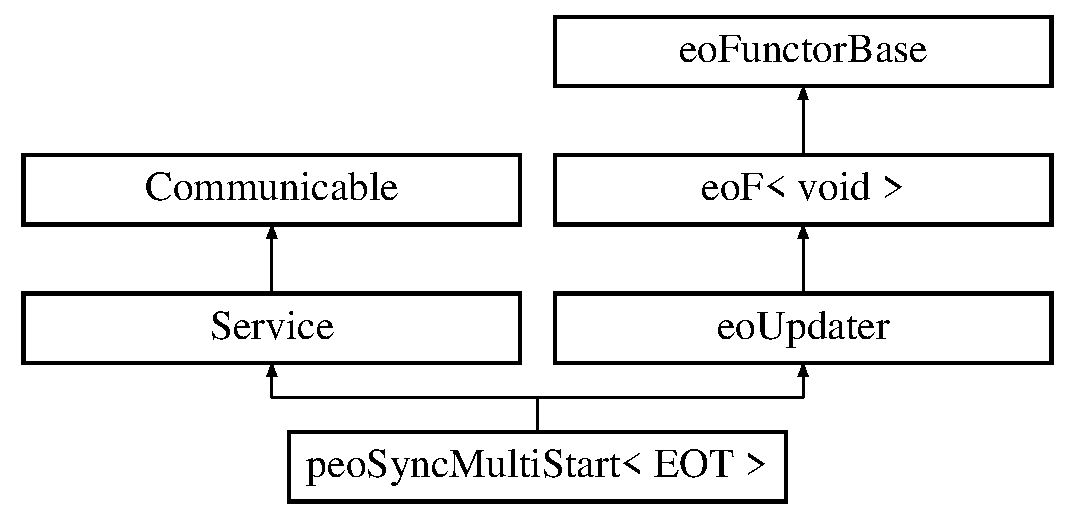
\includegraphics[height=4cm]{classpeoSyncMultiStart}
\end{center}
\end{figure}
\subsection*{Public Member Functions}
\begin{CompactItemize}
\item 
\hyperlink{classpeoSyncMultiStart_d29f94aad3c1f443bfffc8b6aee0704c}{peo\-Sync\-Multi\-Start} (\bf{eo\-Continue}$<$ EOT $>$ \&\_\-\_\-cont, \bf{eo\-Select}$<$ EOT $>$ \&\_\-\_\-select, \bf{eo\-Replacement}$<$ EOT $>$ \&\_\-\_\-replace, \bf{mo\-Algo}$<$ EOT $>$ \&\_\-\_\-ls, \bf{eo\-Pop}$<$ EOT $>$ \&\_\-\_\-pop)
\begin{CompactList}\small\item\em Constructor function - several simple parameters are required for defining the characteristics of the multi-start model. \item\end{CompactList}\item 
void \hyperlink{classpeoSyncMultiStart_76385b33fe514f91cb83f0fbecbeb3c2}{operator()} ()
\begin{CompactList}\small\item\em Operator which synchronously executes the specified algorithm on the individuals selected from the initial population. \item\end{CompactList}\item 
void \hyperlink{classpeoSyncMultiStart_8becfab1922b64708dca5a53e2932a5a}{pack\-Data} ()
\begin{CompactList}\small\item\em Auxiliary function for transferring data between the process requesting the synchronous execution of the specified algorithm and the process which actually executes the algorithm. \item\end{CompactList}\item 
void \hyperlink{classpeoSyncMultiStart_2903a441b77cded266b5fb651e17a5b5}{unpack\-Data} ()
\begin{CompactList}\small\item\em Auxiliary function for transferring data between the process requesting the synchronous execution of the specified algorithm and the process which actually executes the algorithm. \item\end{CompactList}\item 
void \hyperlink{classpeoSyncMultiStart_a4d1c2943c290de540800087b54dc49b}{execute} ()
\begin{CompactList}\small\item\em Auxiliary function for actually executing the specified algorithm on one assigned individual. \item\end{CompactList}\item 
void \hyperlink{classpeoSyncMultiStart_6c48eb0dae741cff7203b65e226f9616}{pack\-Result} ()
\begin{CompactList}\small\item\em Auxiliary function for transferring data between the process requesting the synchronous execution of the specified algorithm and the process which actually executes the algorithm. \item\end{CompactList}\item 
void \hyperlink{classpeoSyncMultiStart_c3cbd1f10a89d1915c5ccf82a2c34a1d}{unpack\-Result} ()
\begin{CompactList}\small\item\em Auxiliary function for transferring data between the process requesting the synchronous execution of the specified algorithm and the process which actually executes the algorithm. \item\end{CompactList}\item 
void \hyperlink{classpeoSyncMultiStart_32ec0d01d3fd8a9932abd68f4781fc94}{notify\-Sending\-Data} ()
\begin{CompactList}\small\item\em Auxiliary function for notifications between the process requesting the synchronous multi-start execution and the processes that performs the actual execution phase. \item\end{CompactList}\item 
void \hyperlink{classpeoSyncMultiStart_fc90282cc4e93cdea8f82fd52dd78fb0}{notify\-Sending\-All\-Resource\-Requests} ()
\begin{CompactList}\small\item\em Auxiliary function for notifications between the process requesting the synchronous multi-start execution and the processes that performs the actual execution phase. \item\end{CompactList}\end{CompactItemize}
\subsection*{Private Attributes}
\begin{CompactItemize}
\item 
\hypertarget{classpeoSyncMultiStart_43f4fa9b125baef6fc8b968dfd16f437}{
\bf{eo\-Continue}$<$ EOT $>$ \& \hyperlink{classpeoSyncMultiStart_43f4fa9b125baef6fc8b968dfd16f437}{cont}}
\label{classpeoSyncMultiStart_43f4fa9b125baef6fc8b968dfd16f437}

\item 
\hypertarget{classpeoSyncMultiStart_8fc9a3d046023ddd077defec3c23ab3b}{
\bf{eo\-Select}$<$ EOT $>$ \& \hyperlink{classpeoSyncMultiStart_8fc9a3d046023ddd077defec3c23ab3b}{select}}
\label{classpeoSyncMultiStart_8fc9a3d046023ddd077defec3c23ab3b}

\item 
\hypertarget{classpeoSyncMultiStart_a375ccea98e9bf2a0854dac27df4522f}{
\bf{eo\-Replacement}$<$ EOT $>$ \& \hyperlink{classpeoSyncMultiStart_a375ccea98e9bf2a0854dac27df4522f}{replace}}
\label{classpeoSyncMultiStart_a375ccea98e9bf2a0854dac27df4522f}

\item 
\hypertarget{classpeoSyncMultiStart_4d317966de767dcc87eee0286ea7f95d}{
\bf{mo\-Algo}$<$ EOT $>$ \& \hyperlink{classpeoSyncMultiStart_4d317966de767dcc87eee0286ea7f95d}{ls}}
\label{classpeoSyncMultiStart_4d317966de767dcc87eee0286ea7f95d}

\item 
\hypertarget{classpeoSyncMultiStart_391178bd6b8a97a08ab4e345f070e967}{
\bf{eo\-Pop}$<$ EOT $>$ \& \hyperlink{classpeoSyncMultiStart_391178bd6b8a97a08ab4e345f070e967}{pop}}
\label{classpeoSyncMultiStart_391178bd6b8a97a08ab4e345f070e967}

\item 
\hypertarget{classpeoSyncMultiStart_dbcc1a069ec72ecd8d40c392640d84b3}{
\bf{eo\-Pop}$<$ EOT $>$ \hyperlink{classpeoSyncMultiStart_dbcc1a069ec72ecd8d40c392640d84b3}{sel}}
\label{classpeoSyncMultiStart_dbcc1a069ec72ecd8d40c392640d84b3}

\item 
\hypertarget{classpeoSyncMultiStart_ca10f6d258105e3c4f0d1660db5b7679}{
\bf{eo\-Pop}$<$ EOT $>$ \hyperlink{classpeoSyncMultiStart_ca10f6d258105e3c4f0d1660db5b7679}{impr\_\-sel}}
\label{classpeoSyncMultiStart_ca10f6d258105e3c4f0d1660db5b7679}

\item 
\hypertarget{classpeoSyncMultiStart_2c2ebe46470d1425f0409897deab435b}{
EOT \hyperlink{classpeoSyncMultiStart_2c2ebe46470d1425f0409897deab435b}{sol}}
\label{classpeoSyncMultiStart_2c2ebe46470d1425f0409897deab435b}

\item 
\hypertarget{classpeoSyncMultiStart_64191ef79b7b589964ac9c3e23ae6718}{
unsigned \hyperlink{classpeoSyncMultiStart_64191ef79b7b589964ac9c3e23ae6718}{idx}}
\label{classpeoSyncMultiStart_64191ef79b7b589964ac9c3e23ae6718}

\item 
\hypertarget{classpeoSyncMultiStart_773eb9097550d9444f25ca8f48997a30}{
unsigned \hyperlink{classpeoSyncMultiStart_773eb9097550d9444f25ca8f48997a30}{num\_\-term}}
\label{classpeoSyncMultiStart_773eb9097550d9444f25ca8f48997a30}

\end{CompactItemize}


\subsection{Detailed Description}
\subsubsection*{template$<$class EOT$>$ class peo\-Sync\-Multi\-Start$<$ EOT $>$}

The \hyperlink{classpeoSyncMultiStart}{peo\-Sync\-Multi\-Start} class provides the basis for implementing the synchronous multi-start model, for launching several solution-based algorithms in parallel on a specified initial population. 

As a simple example, several hill climbing algorithms may be synchronously launched on the specified population, each algorithm acting upon one individual only, the final result being integrated back in the population. A \hyperlink{classpeoSyncMultiStart}{peo\-Sync\-Multi\-Start} object can be specified as checkpoint object for a classic Paradis\-EO evolutionary algorithm thus allowing for simple hybridization schemes which combine the evolutionary approach with a local search approach, for example, executed at the end of each generation. 



Definition at line 64 of file peo\-Sync\-Multi\-Start.h.

\subsection{Constructor \& Destructor Documentation}
\hypertarget{classpeoSyncMultiStart_d29f94aad3c1f443bfffc8b6aee0704c}{
\index{peoSyncMultiStart@{peo\-Sync\-Multi\-Start}!peoSyncMultiStart@{peoSyncMultiStart}}
\index{peoSyncMultiStart@{peoSyncMultiStart}!peoSyncMultiStart@{peo\-Sync\-Multi\-Start}}
\subsubsection[peoSyncMultiStart]{\setlength{\rightskip}{0pt plus 5cm}template$<$class EOT$>$ \hyperlink{classpeoSyncMultiStart}{peo\-Sync\-Multi\-Start}$<$ EOT $>$::\hyperlink{classpeoSyncMultiStart}{peo\-Sync\-Multi\-Start} (\bf{eo\-Continue}$<$ EOT $>$ \& {\em \_\-\_\-cont}, \bf{eo\-Select}$<$ EOT $>$ \& {\em \_\-\_\-select}, \bf{eo\-Replacement}$<$ EOT $>$ \& {\em \_\-\_\-replace}, \bf{mo\-Algo}$<$ EOT $>$ \& {\em \_\-\_\-ls}, \bf{eo\-Pop}$<$ EOT $>$ \& {\em \_\-\_\-pop})}}
\label{classpeoSyncMultiStart_d29f94aad3c1f443bfffc8b6aee0704c}


Constructor function - several simple parameters are required for defining the characteristics of the multi-start model. 

\begin{Desc}
\item[Parameters:]
\begin{description}
\item[{\em eo\-Continue$<$}]EOT $>$\& \_\-\_\-cont - defined for including further functionality - no semantics associated at this time; \item[{\em eo\-Select$<$}]EOT $>$\& \_\-\_\-select - selection strategy for obtaining a subset of the initial population on which to apply the specified algorithm; \item[{\em eo\-Replacement$<$}]EOT $>$\& \_\-\_\-replace - replacement strategy for integrating the resulting individuals in the initial population; \item[{\em mo\-Algo$<$}]EOT $>$\& \_\-\_\-ls - algorithm to be applied on each of the selected individuals - a {\bf mo\-Algo$<$ EOT $>$}-derived object must be specified; \item[{\em eo\-Pop$<$}]EOT $>$\& \_\-\_\-pop - the initial population from which the individuals are selected for applying the specified algorithm. \end{description}
\end{Desc}


Definition at line 134 of file peo\-Sync\-Multi\-Start.h.

\subsection{Member Function Documentation}
\hypertarget{classpeoSyncMultiStart_76385b33fe514f91cb83f0fbecbeb3c2}{
\index{peoSyncMultiStart@{peo\-Sync\-Multi\-Start}!operator()@{operator()}}
\index{operator()@{operator()}!peoSyncMultiStart@{peo\-Sync\-Multi\-Start}}
\subsubsection[operator()]{\setlength{\rightskip}{0pt plus 5cm}template$<$class EOT$>$ void \hyperlink{classpeoSyncMultiStart}{peo\-Sync\-Multi\-Start}$<$ EOT $>$::operator() ()\hspace{0.3cm}{\tt  \mbox{[}virtual\mbox{]}}}}
\label{classpeoSyncMultiStart_76385b33fe514f91cb83f0fbecbeb3c2}


Operator which synchronously executes the specified algorithm on the individuals selected from the initial population. 

There is no need to explicitly call the operator - automatically called as checkpoint operator. 

Implements \bf{eo\-F$<$ void $>$}.

Definition at line 189 of file peo\-Sync\-Multi\-Start.h.

References peo\-Sync\-Multi\-Start$<$ EOT $>$::idx, peo\-Sync\-Multi\-Start$<$ EOT $>$::impr\_\-sel, peo\-Sync\-Multi\-Start$<$ EOT $>$::num\_\-term, peo\-Sync\-Multi\-Start$<$ EOT $>$::pop, Service::request\-Resource\-Request(), peo\-Sync\-Multi\-Start$<$ EOT $>$::sel, peo\-Sync\-Multi\-Start$<$ EOT $>$::select, and Communicable::stop().\hypertarget{classpeoSyncMultiStart_8becfab1922b64708dca5a53e2932a5a}{
\index{peoSyncMultiStart@{peo\-Sync\-Multi\-Start}!packData@{packData}}
\index{packData@{packData}!peoSyncMultiStart@{peo\-Sync\-Multi\-Start}}
\subsubsection[packData]{\setlength{\rightskip}{0pt plus 5cm}template$<$class EOT$>$ void \hyperlink{classpeoSyncMultiStart}{peo\-Sync\-Multi\-Start}$<$ EOT $>$::pack\-Data ()\hspace{0.3cm}{\tt  \mbox{[}virtual\mbox{]}}}}
\label{classpeoSyncMultiStart_8becfab1922b64708dca5a53e2932a5a}


Auxiliary function for transferring data between the process requesting the synchronous execution of the specified algorithm and the process which actually executes the algorithm. 

There is no need to explicitly call the function. 

Reimplemented from \hyperlink{classService_aea4b8f7f8fb88e83862ee4bfd9ab207}{Service}.

Definition at line 148 of file peo\-Sync\-Multi\-Start.h.

References peo\-Sync\-Multi\-Start$<$ EOT $>$::idx, and peo\-Sync\-Multi\-Start$<$ EOT $>$::sel.\hypertarget{classpeoSyncMultiStart_2903a441b77cded266b5fb651e17a5b5}{
\index{peoSyncMultiStart@{peo\-Sync\-Multi\-Start}!unpackData@{unpackData}}
\index{unpackData@{unpackData}!peoSyncMultiStart@{peo\-Sync\-Multi\-Start}}
\subsubsection[unpackData]{\setlength{\rightskip}{0pt plus 5cm}template$<$class EOT$>$ void \hyperlink{classpeoSyncMultiStart}{peo\-Sync\-Multi\-Start}$<$ EOT $>$::unpack\-Data ()\hspace{0.3cm}{\tt  \mbox{[}virtual\mbox{]}}}}
\label{classpeoSyncMultiStart_2903a441b77cded266b5fb651e17a5b5}


Auxiliary function for transferring data between the process requesting the synchronous execution of the specified algorithm and the process which actually executes the algorithm. 

There is no need to explicitly call the function. 

Reimplemented from \hyperlink{classService_3bd87b444710813d30fd754d4d0b4df3}{Service}.

Definition at line 154 of file peo\-Sync\-Multi\-Start.h.

References peo\-Sync\-Multi\-Start$<$ EOT $>$::sol.\hypertarget{classpeoSyncMultiStart_a4d1c2943c290de540800087b54dc49b}{
\index{peoSyncMultiStart@{peo\-Sync\-Multi\-Start}!execute@{execute}}
\index{execute@{execute}!peoSyncMultiStart@{peo\-Sync\-Multi\-Start}}
\subsubsection[execute]{\setlength{\rightskip}{0pt plus 5cm}template$<$class EOT$>$ void \hyperlink{classpeoSyncMultiStart}{peo\-Sync\-Multi\-Start}$<$ EOT $>$::execute ()\hspace{0.3cm}{\tt  \mbox{[}virtual\mbox{]}}}}
\label{classpeoSyncMultiStart_a4d1c2943c290de540800087b54dc49b}


Auxiliary function for actually executing the specified algorithm on one assigned individual. 

There is no need to explicitly call the function. 

Reimplemented from \hyperlink{classService_e4f2894e6121e60f38d41cfbd7447ae4}{Service}.

Definition at line 160 of file peo\-Sync\-Multi\-Start.h.

References peo\-Sync\-Multi\-Start$<$ EOT $>$::ls, and peo\-Sync\-Multi\-Start$<$ EOT $>$::sol.\hypertarget{classpeoSyncMultiStart_6c48eb0dae741cff7203b65e226f9616}{
\index{peoSyncMultiStart@{peo\-Sync\-Multi\-Start}!packResult@{packResult}}
\index{packResult@{packResult}!peoSyncMultiStart@{peo\-Sync\-Multi\-Start}}
\subsubsection[packResult]{\setlength{\rightskip}{0pt plus 5cm}template$<$class EOT$>$ void \hyperlink{classpeoSyncMultiStart}{peo\-Sync\-Multi\-Start}$<$ EOT $>$::pack\-Result ()\hspace{0.3cm}{\tt  \mbox{[}virtual\mbox{]}}}}
\label{classpeoSyncMultiStart_6c48eb0dae741cff7203b65e226f9616}


Auxiliary function for transferring data between the process requesting the synchronous execution of the specified algorithm and the process which actually executes the algorithm. 

There is no need to explicitly call the function. 

Reimplemented from \hyperlink{classService_e5e4f90b2315e15c2a2913bd370f4cf5}{Service}.

Definition at line 166 of file peo\-Sync\-Multi\-Start.h.

References peo\-Sync\-Multi\-Start$<$ EOT $>$::sol.\hypertarget{classpeoSyncMultiStart_c3cbd1f10a89d1915c5ccf82a2c34a1d}{
\index{peoSyncMultiStart@{peo\-Sync\-Multi\-Start}!unpackResult@{unpackResult}}
\index{unpackResult@{unpackResult}!peoSyncMultiStart@{peo\-Sync\-Multi\-Start}}
\subsubsection[unpackResult]{\setlength{\rightskip}{0pt plus 5cm}template$<$class EOT$>$ void \hyperlink{classpeoSyncMultiStart}{peo\-Sync\-Multi\-Start}$<$ EOT $>$::unpack\-Result ()\hspace{0.3cm}{\tt  \mbox{[}virtual\mbox{]}}}}
\label{classpeoSyncMultiStart_c3cbd1f10a89d1915c5ccf82a2c34a1d}


Auxiliary function for transferring data between the process requesting the synchronous execution of the specified algorithm and the process which actually executes the algorithm. 

There is no need to explicitly call the function. 

Reimplemented from \hyperlink{classService_45c06344edbfa482b91f68e2035a6099}{Service}.

Definition at line 172 of file peo\-Sync\-Multi\-Start.h.

References Service::get\-Owner(), peo\-Sync\-Multi\-Start$<$ EOT $>$::impr\_\-sel, peo\-Sync\-Multi\-Start$<$ EOT $>$::num\_\-term, peo\-Sync\-Multi\-Start$<$ EOT $>$::pop, peo\-Sync\-Multi\-Start$<$ EOT $>$::replace, Communicable::resume(), peo\-Sync\-Multi\-Start$<$ EOT $>$::sel, Thread::set\-Active(), and peo\-Sync\-Multi\-Start$<$ EOT $>$::sol.\hypertarget{classpeoSyncMultiStart_32ec0d01d3fd8a9932abd68f4781fc94}{
\index{peoSyncMultiStart@{peo\-Sync\-Multi\-Start}!notifySendingData@{notifySendingData}}
\index{notifySendingData@{notifySendingData}!peoSyncMultiStart@{peo\-Sync\-Multi\-Start}}
\subsubsection[notifySendingData]{\setlength{\rightskip}{0pt plus 5cm}template$<$class EOT$>$ void \hyperlink{classpeoSyncMultiStart}{peo\-Sync\-Multi\-Start}$<$ EOT $>$::notify\-Sending\-Data ()\hspace{0.3cm}{\tt  \mbox{[}virtual\mbox{]}}}}
\label{classpeoSyncMultiStart_32ec0d01d3fd8a9932abd68f4781fc94}


Auxiliary function for notifications between the process requesting the synchronous multi-start execution and the processes that performs the actual execution phase. 

There is no need to explicitly call the function. 

Reimplemented from \hyperlink{classService_81ad4d6ebb50045b8977e2ab74826f30}{Service}.

Definition at line 200 of file peo\-Sync\-Multi\-Start.h.\hypertarget{classpeoSyncMultiStart_fc90282cc4e93cdea8f82fd52dd78fb0}{
\index{peoSyncMultiStart@{peo\-Sync\-Multi\-Start}!notifySendingAllResourceRequests@{notifySendingAllResourceRequests}}
\index{notifySendingAllResourceRequests@{notifySendingAllResourceRequests}!peoSyncMultiStart@{peo\-Sync\-Multi\-Start}}
\subsubsection[notifySendingAllResourceRequests]{\setlength{\rightskip}{0pt plus 5cm}template$<$class EOT$>$ void \hyperlink{classpeoSyncMultiStart}{peo\-Sync\-Multi\-Start}$<$ EOT $>$::notify\-Sending\-All\-Resource\-Requests ()\hspace{0.3cm}{\tt  \mbox{[}virtual\mbox{]}}}}
\label{classpeoSyncMultiStart_fc90282cc4e93cdea8f82fd52dd78fb0}


Auxiliary function for notifications between the process requesting the synchronous multi-start execution and the processes that performs the actual execution phase. 

There is no need to explicitly call the function. 

Reimplemented from \hyperlink{classService_f94cc8a5c2665d4574041737e61e9ffc}{Service}.

Definition at line 205 of file peo\-Sync\-Multi\-Start.h.

References Service::get\-Owner(), and Thread::set\-Passive().

The documentation for this class was generated from the following file:\begin{CompactItemize}
\item 
peo\-Sync\-Multi\-Start.h\end{CompactItemize}

\hypertarget{classpeoTransform}{
\section{peo\-Transform$<$ EOT $>$ Class Template Reference}
\label{classpeoTransform}\index{peoTransform@{peoTransform}}
}
Class for a parallel transform.  


{\tt \#include $<$peo\-Transform.h$>$}

Inheritance diagram for peo\-Transform$<$ EOT $>$::\begin{figure}[H]
\begin{center}
\leavevmode
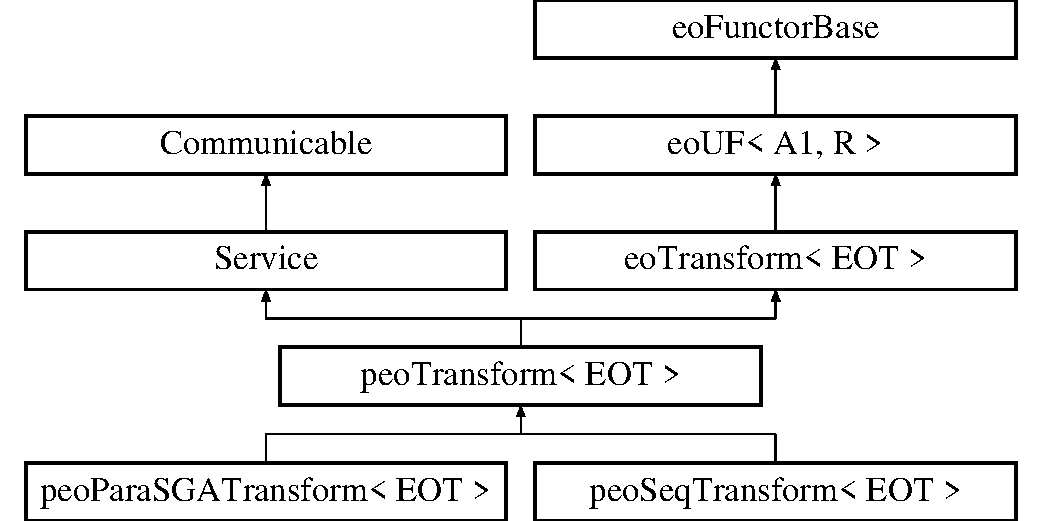
\includegraphics[height=4cm]{classpeoTransform}
\end{center}
\end{figure}
\subsection*{Public Member Functions}
\begin{CompactItemize}
\item 
\hyperlink{classpeoTransform_755989a2d080903d0cade75643de0788}{peo\-Transform} (\bf{eo\-Quad\-Op}$<$ EOT $>$ \&\_\-\_\-cross, double \_\-\_\-cross\_\-rate, \bf{eo\-Mon\-Op}$<$ EOT $>$ \&\_\-\_\-mut, double \_\-\_\-mut\_\-rate)
\begin{CompactList}\small\item\em Constructor. \item\end{CompactList}\item 
void \hyperlink{classpeoTransform_9322aa28ad272289132e342624a0adb4}{operator()} (\bf{eo\-Pop}$<$ EOT $>$ \&\_\-\_\-pop)
\begin{CompactList}\small\item\em Operator. \item\end{CompactList}\item 
\hypertarget{classpeoTransform_c1101d10a36ce4255b874bcd9725021e}{
void \hyperlink{classpeoTransform_c1101d10a36ce4255b874bcd9725021e}{pack\-Data} ()}
\label{classpeoTransform_c1101d10a36ce4255b874bcd9725021e}

\begin{CompactList}\small\item\em \doxyref{Function} realizing packages of data. \item\end{CompactList}\item 
\hypertarget{classpeoTransform_a804631492e08053162a196877587aef}{
void \hyperlink{classpeoTransform_a804631492e08053162a196877587aef}{unpack\-Data} ()}
\label{classpeoTransform_a804631492e08053162a196877587aef}

\begin{CompactList}\small\item\em \doxyref{Function} reconstituting packages of data. \item\end{CompactList}\item 
\hypertarget{classpeoTransform_85c2cbc76f803b2b5cb2bc8cbc214136}{
void \hyperlink{classpeoTransform_85c2cbc76f803b2b5cb2bc8cbc214136}{execute} ()}
\label{classpeoTransform_85c2cbc76f803b2b5cb2bc8cbc214136}

\begin{CompactList}\small\item\em \doxyref{Function} which executes the algorithm. \item\end{CompactList}\item 
\hypertarget{classpeoTransform_bdae056027406ba9f489e2bef115fd08}{
void \hyperlink{classpeoTransform_bdae056027406ba9f489e2bef115fd08}{pack\-Result} ()}
\label{classpeoTransform_bdae056027406ba9f489e2bef115fd08}

\begin{CompactList}\small\item\em \doxyref{Function} realizing packages of the result. \item\end{CompactList}\item 
\hypertarget{classpeoTransform_e0244425e846c5679c901b61e4252814}{
void \hyperlink{classpeoTransform_e0244425e846c5679c901b61e4252814}{unpack\-Result} ()}
\label{classpeoTransform_e0244425e846c5679c901b61e4252814}

\begin{CompactList}\small\item\em \doxyref{Function} reconstituting packages of result. \item\end{CompactList}\item 
\hypertarget{classpeoTransform_77508f186476181ec2c6a8230961eede}{
void \hyperlink{classpeoTransform_77508f186476181ec2c6a8230961eede}{notify\-Sending\-Data} ()}
\label{classpeoTransform_77508f186476181ec2c6a8230961eede}

\begin{CompactList}\small\item\em \doxyref{Function} notify\-Sending\-Data. \item\end{CompactList}\item 
\hypertarget{classpeoTransform_19990af963b6604d1175290fe6725335}{
void \hyperlink{classpeoTransform_19990af963b6604d1175290fe6725335}{notify\-Sending\-All\-Resource\-Requests} ()}
\label{classpeoTransform_19990af963b6604d1175290fe6725335}

\begin{CompactList}\small\item\em \doxyref{Function} notify\-Sending\-All\-Resource\-Requests. \item\end{CompactList}\end{CompactItemize}
\subsection*{Private Attributes}
\begin{CompactItemize}
\item 
\bf{eo\-Quad\-Op}$<$ EOT $>$ \& \hyperlink{classpeoTransform_d2fce5199b61f599fd89cf54d6fcd312}{cross}
\item 
\hypertarget{classpeoTransform_3336251fb3433a8405ea75f3a8bed04d}{
double \hyperlink{classpeoTransform_3336251fb3433a8405ea75f3a8bed04d}{cross\_\-rate}}
\label{classpeoTransform_3336251fb3433a8405ea75f3a8bed04d}

\item 
\hypertarget{classpeoTransform_3d1ea5c8a6aa95bf051051361908a9c6}{
\bf{eo\-Mon\-Op}$<$ EOT $>$ \& \hyperlink{classpeoTransform_3d1ea5c8a6aa95bf051051361908a9c6}{mut}}
\label{classpeoTransform_3d1ea5c8a6aa95bf051051361908a9c6}

\item 
\hypertarget{classpeoTransform_0b0802dfc4a3ec664c8fccf10bb1842a}{
double \hyperlink{classpeoTransform_0b0802dfc4a3ec664c8fccf10bb1842a}{mut\_\-rate}}
\label{classpeoTransform_0b0802dfc4a3ec664c8fccf10bb1842a}

\item 
\hypertarget{classpeoTransform_0acac288337aec3d0d853565924a365d}{
unsigned \hyperlink{classpeoTransform_0acac288337aec3d0d853565924a365d}{idx}}
\label{classpeoTransform_0acac288337aec3d0d853565924a365d}

\item 
\hypertarget{classpeoTransform_0916042d3500452082ad19fd5ce5e161}{
\bf{eo\-Pop}$<$ EOT $>$ $\ast$ \hyperlink{classpeoTransform_0916042d3500452082ad19fd5ce5e161}{pop}}
\label{classpeoTransform_0916042d3500452082ad19fd5ce5e161}

\item 
\hypertarget{classpeoTransform_88c563f77e5c25b70b6cb619ec97185f}{
EOT \hyperlink{classpeoTransform_88c563f77e5c25b70b6cb619ec97185f}{father}}
\label{classpeoTransform_88c563f77e5c25b70b6cb619ec97185f}

\item 
\hypertarget{classpeoTransform_5c754343fa9a3580632d6b9e8f1bafaa}{
EOT \hyperlink{classpeoTransform_5c754343fa9a3580632d6b9e8f1bafaa}{mother}}
\label{classpeoTransform_5c754343fa9a3580632d6b9e8f1bafaa}

\item 
\hypertarget{classpeoTransform_6a02c2c2de16c5825058e06d146c5cd9}{
unsigned \hyperlink{classpeoTransform_6a02c2c2de16c5825058e06d146c5cd9}{num\_\-term}}
\label{classpeoTransform_6a02c2c2de16c5825058e06d146c5cd9}

\end{CompactItemize}


\subsection{Detailed Description}
\subsubsection*{template$<$class EOT$>$ class peo\-Transform$<$ EOT $>$}

Class for a parallel transform. 

\begin{Desc}
\item[See also:]\hyperlink{classService}{Service} \doxyref{eo\-Transform} \end{Desc}
\begin{Desc}
\item[Version:]1.1 \end{Desc}
\begin{Desc}
\item[Date:]january 2008 \end{Desc}




Definition at line 53 of file peo\-Transform.h.

\subsection{Constructor \& Destructor Documentation}
\hypertarget{classpeoTransform_755989a2d080903d0cade75643de0788}{
\index{peoTransform@{peo\-Transform}!peoTransform@{peoTransform}}
\index{peoTransform@{peoTransform}!peoTransform@{peo\-Transform}}
\subsubsection[peoTransform]{\setlength{\rightskip}{0pt plus 5cm}template$<$class EOT$>$ \hyperlink{classpeoTransform}{peo\-Transform}$<$ EOT $>$::\hyperlink{classpeoTransform}{peo\-Transform} (\bf{eo\-Quad\-Op}$<$ EOT $>$ \& {\em \_\-\_\-cross}, double {\em \_\-\_\-cross\_\-rate}, \bf{eo\-Mon\-Op}$<$ EOT $>$ \& {\em \_\-\_\-mut}, double {\em \_\-\_\-mut\_\-rate})}}
\label{classpeoTransform_755989a2d080903d0cade75643de0788}


Constructor. 

\begin{Desc}
\item[Parameters:]
\begin{description}
\item[{\em eo\-Quad\-Op$<$}]EOT $>$\& \_\-\_\-cross \item[{\em double}]\_\-\_\-cross\_\-rate \item[{\em eo\-Mon\-Op$<$}]EOT $>$\& \_\-\_\-mut \item[{\em double}]\_\-\_\-mut\_\-rate \end{description}
\end{Desc}


Definition at line 108 of file peo\-Transform.h.

\subsection{Member Function Documentation}
\hypertarget{classpeoTransform_9322aa28ad272289132e342624a0adb4}{
\index{peoTransform@{peo\-Transform}!operator()@{operator()}}
\index{operator()@{operator()}!peoTransform@{peo\-Transform}}
\subsubsection[operator()]{\setlength{\rightskip}{0pt plus 5cm}template$<$class EOT$>$ void \hyperlink{classpeoTransform}{peo\-Transform}$<$ EOT $>$::operator() (\bf{eo\-Pop}$<$ EOT $>$ \& {\em \_\-\_\-pop})}}
\label{classpeoTransform_9322aa28ad272289132e342624a0adb4}


Operator. 

\begin{Desc}
\item[Parameters:]
\begin{description}
\item[{\em eo\-Pop$<$}]EOT $>$\& \_\-\_\-pop \end{description}
\end{Desc}


Definition at line 176 of file peo\-Transform.h.

References peo\-Transform$<$ EOT $>$::idx, peo\-Transform$<$ EOT $>$::num\_\-term, peo\-Transform$<$ EOT $>$::pop, Service::request\-Resource\-Request(), and Communicable::stop().

\subsection{Member Data Documentation}
\hypertarget{classpeoTransform_d2fce5199b61f599fd89cf54d6fcd312}{
\index{peoTransform@{peo\-Transform}!cross@{cross}}
\index{cross@{cross}!peoTransform@{peo\-Transform}}
\subsubsection[cross]{\setlength{\rightskip}{0pt plus 5cm}template$<$class EOT$>$ \bf{eo\-Quad\-Op}$<$ EOT $>$\& \hyperlink{classpeoTransform}{peo\-Transform}$<$ EOT $>$::\hyperlink{classpeoTransform_d2fce5199b61f599fd89cf54d6fcd312}{cross}\hspace{0.3cm}{\tt  \mbox{[}private\mbox{]}}}}
\label{classpeoTransform_d2fce5199b61f599fd89cf54d6fcd312}


\begin{Desc}
\item[Parameters:]
\begin{description}
\item[{\em eo\-Quad\-Op$<$}]EOT $>$\& cross \item[{\em double}]cross\_\-rate \item[{\em eo\-Mon\-Op$<$}]EOT $>$\& mut \item[{\em double}]mut\_\-rate \item[{\em unsigned}]idx \item[{\em eo\-Pop$<$}]EOT $>$$\ast$ pop \item[{\em EOT}]father \item[{\em mother}]\item[{\em unsigned}]num\_\-term \end{description}
\end{Desc}


Definition at line 98 of file peo\-Transform.h.

Referenced by peo\-Transform$<$ EOT $>$::execute().

The documentation for this class was generated from the following file:\begin{CompactItemize}
\item 
peo\-Transform.h\end{CompactItemize}

\hypertarget{structRandomExplorationAlgorithm}{
\section{Random\-Exploration\-Algorithm Struct Reference}
\label{structRandomExplorationAlgorithm}\index{RandomExplorationAlgorithm@{RandomExplorationAlgorithm}}
}
\subsection*{Public Member Functions}
\begin{CompactItemize}
\item 
\hypertarget{structRandomExplorationAlgorithm_ed4847c164759fbb1168948d3620037c}{
\hyperlink{structRandomExplorationAlgorithm_ed4847c164759fbb1168948d3620037c}{Random\-Exploration\-Algorithm} (\hyperlink{classpeoPopEval}{peo\-Pop\-Eval}$<$ \bf{Route} $>$ \&\_\-\_\-pop\-Eval, \hyperlink{classpeoSynchronousMultiStart}{peo\-Synchronous\-Multi\-Start}$<$ \bf{Route} $>$ \&ext\-Parallel\-Execution)}
\label{structRandomExplorationAlgorithm_ed4847c164759fbb1168948d3620037c}

\item 
\hypertarget{structRandomExplorationAlgorithm_3a7b3cc174726fff45985854c3d1b812}{
void \hyperlink{structRandomExplorationAlgorithm_3a7b3cc174726fff45985854c3d1b812}{operator()} ()}
\label{structRandomExplorationAlgorithm_3a7b3cc174726fff45985854c3d1b812}

\end{CompactItemize}
\subsection*{Public Attributes}
\begin{CompactItemize}
\item 
\hypertarget{structRandomExplorationAlgorithm_e9fbab7402f290c62224cedebd9de0a4}{
\hyperlink{classpeoPopEval}{peo\-Pop\-Eval}$<$ \bf{Route} $>$ \& \hyperlink{structRandomExplorationAlgorithm_e9fbab7402f290c62224cedebd9de0a4}{pop\-Eval}}
\label{structRandomExplorationAlgorithm_e9fbab7402f290c62224cedebd9de0a4}

\item 
\hypertarget{structRandomExplorationAlgorithm_e36e837e956772738773364cd71201de}{
\hyperlink{classpeoSynchronousMultiStart}{peo\-Synchronous\-Multi\-Start}$<$ \bf{Route} $>$ \& \hyperlink{structRandomExplorationAlgorithm_e36e837e956772738773364cd71201de}{parallel\-Execution}}
\label{structRandomExplorationAlgorithm_e36e837e956772738773364cd71201de}

\end{CompactItemize}


\subsection{Detailed Description}




Definition at line 56 of file Lesson\-Parallel\-Algorithm/main.cpp.

The documentation for this struct was generated from the following file:\begin{CompactItemize}
\item 
Lesson\-Parallel\-Algorithm/main.cpp\end{CompactItemize}

\hypertarget{classReactiveThread}{
\section{Reactive\-Thread Class Reference}
\label{classReactiveThread}\index{ReactiveThread@{ReactiveThread}}
}
Inheritance diagram for Reactive\-Thread::\begin{figure}[H]
\begin{center}
\leavevmode
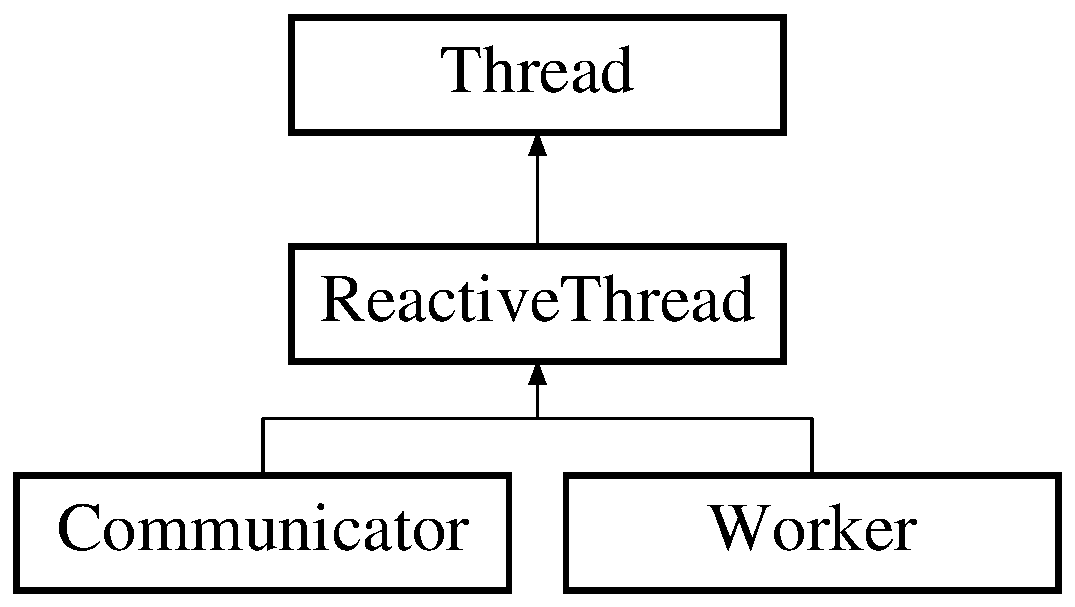
\includegraphics[height=3cm]{classReactiveThread}
\end{center}
\end{figure}
\subsection*{Public Member Functions}
\begin{CompactItemize}
\item 
\hypertarget{classReactiveThread_77381649429941c99a3e3d568113d6cf}{
\hyperlink{classReactiveThread_77381649429941c99a3e3d568113d6cf}{Reactive\-Thread} ()}
\label{classReactiveThread_77381649429941c99a3e3d568113d6cf}

\item 
\hypertarget{classReactiveThread_8263c2a32d8c99a49a05f1a7717d4262}{
void \hyperlink{classReactiveThread_8263c2a32d8c99a49a05f1a7717d4262}{sleep} ()}
\label{classReactiveThread_8263c2a32d8c99a49a05f1a7717d4262}

\item 
\hypertarget{classReactiveThread_a724a54575de10f09cc03ab7aa4e59ce}{
void \hyperlink{classReactiveThread_a724a54575de10f09cc03ab7aa4e59ce}{wake\-Up} ()}
\label{classReactiveThread_a724a54575de10f09cc03ab7aa4e59ce}

\end{CompactItemize}
\subsection*{Private Attributes}
\begin{CompactItemize}
\item 
\hypertarget{classReactiveThread_915e5a42dc8cb1bcf6738d5fe883a4e7}{
sem\_\-t \hyperlink{classReactiveThread_915e5a42dc8cb1bcf6738d5fe883a4e7}{sem}}
\label{classReactiveThread_915e5a42dc8cb1bcf6738d5fe883a4e7}

\end{CompactItemize}


\subsection{Detailed Description}




Definition at line 45 of file reac\_\-thread.h.

The documentation for this class was generated from the following files:\begin{CompactItemize}
\item 
reac\_\-thread.h\item 
reac\_\-thread.cpp\end{CompactItemize}

\hypertarget{classRingTopology}{
\section{Ring\-Topology Class Reference}
\label{classRingTopology}\index{RingTopology@{RingTopology}}
}
Inheritance diagram for Ring\-Topology::\begin{figure}[H]
\begin{center}
\leavevmode
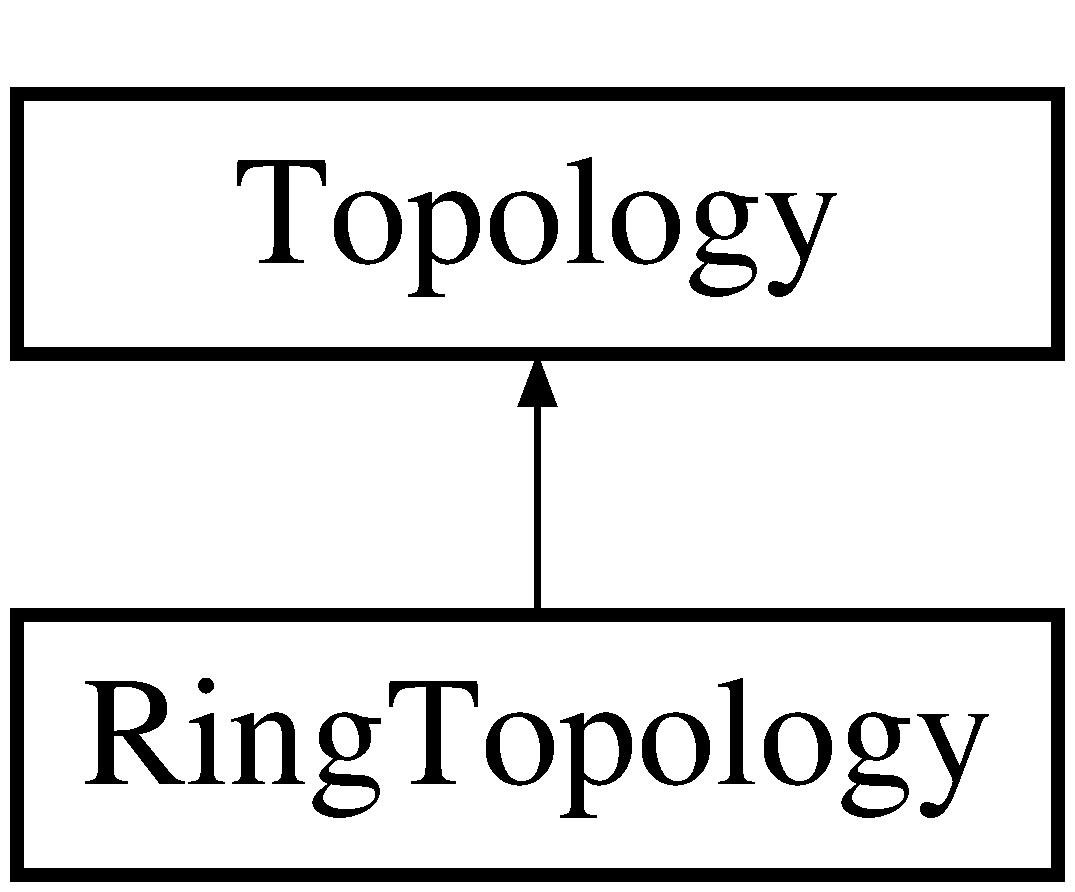
\includegraphics[height=2cm]{classRingTopology}
\end{center}
\end{figure}
\subsection*{Public Member Functions}
\begin{CompactItemize}
\item 
\hypertarget{classRingTopology_292a7746993788f96042f2f628cfcbc5}{
void \hyperlink{classRingTopology_292a7746993788f96042f2f628cfcbc5}{set\-Neighbors} (\hyperlink{classCooperative}{Cooperative} $\ast$\_\-\_\-mig, std::vector$<$ \hyperlink{classCooperative}{Cooperative} $\ast$ $>$ \&\_\-\_\-from, std::vector$<$ \hyperlink{classCooperative}{Cooperative} $\ast$ $>$ \&\_\-\_\-to)}
\label{classRingTopology_292a7746993788f96042f2f628cfcbc5}

\end{CompactItemize}


\subsection{Detailed Description}




Definition at line 42 of file ring\_\-topo.h.

The documentation for this class was generated from the following files:\begin{CompactItemize}
\item 
ring\_\-topo.h\item 
ring\_\-topo.cpp\end{CompactItemize}

\hypertarget{classRunner}{
\section{Runner Class Reference}
\label{classRunner}\index{Runner@{Runner}}
}
Inheritance diagram for Runner::\begin{figure}[H]
\begin{center}
\leavevmode
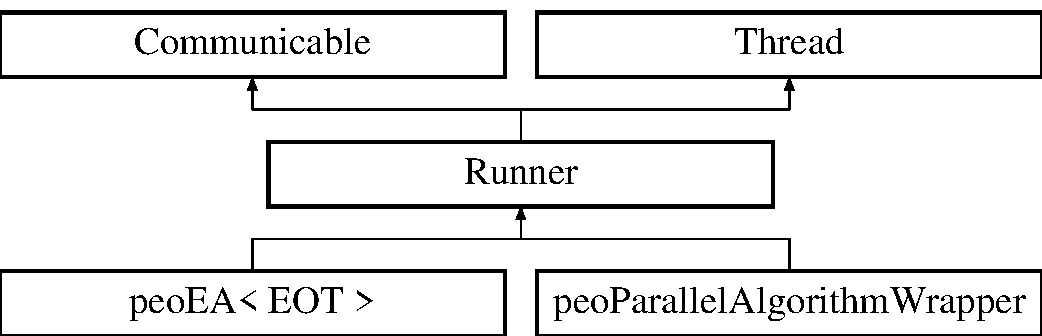
\includegraphics[height=3cm]{classRunner}
\end{center}
\end{figure}
\subsection*{Public Member Functions}
\begin{CompactItemize}
\item 
\hypertarget{classRunner_7acb8258c21da9daa62f9a177a2e5acd}{
\hyperlink{classRunner_7acb8258c21da9daa62f9a177a2e5acd}{Runner} ()}
\label{classRunner_7acb8258c21da9daa62f9a177a2e5acd}

\item 
\hypertarget{classRunner_7dc4419051fcc5cc9dadd54ecc9cd47d}{
void \hyperlink{classRunner_7dc4419051fcc5cc9dadd54ecc9cd47d}{start} ()}
\label{classRunner_7dc4419051fcc5cc9dadd54ecc9cd47d}

\item 
\hypertarget{classRunner_5bc239db2be753b77369fa9a038769fd}{
void \hyperlink{classRunner_5bc239db2be753b77369fa9a038769fd}{wait\-Starting} ()}
\label{classRunner_5bc239db2be753b77369fa9a038769fd}

\item 
\hypertarget{classRunner_40adbfb7d6944189b4fff60b02e669ca}{
bool \hyperlink{classRunner_40adbfb7d6944189b4fff60b02e669ca}{is\-Local} ()}
\label{classRunner_40adbfb7d6944189b4fff60b02e669ca}

\item 
\hypertarget{classRunner_0f133e75c28fb8264549814f80608e68}{
void \hyperlink{classRunner_0f133e75c28fb8264549814f80608e68}{terminate} ()}
\label{classRunner_0f133e75c28fb8264549814f80608e68}

\item 
\hypertarget{classRunner_5026c74eec184e3a15cb3c0ec4200a57}{
RUNNER\_\-ID \hyperlink{classRunner_5026c74eec184e3a15cb3c0ec4200a57}{get\-ID} ()}
\label{classRunner_5026c74eec184e3a15cb3c0ec4200a57}

\item 
\hypertarget{classRunner_2ad6d199d684d6f34347fc202ffe2fa3}{
void \hyperlink{classRunner_2ad6d199d684d6f34347fc202ffe2fa3}{pack\-Termination} ()}
\label{classRunner_2ad6d199d684d6f34347fc202ffe2fa3}

\item 
\hypertarget{classRunner_3591be473e0fcee1105fb57319b529aa}{
void \hyperlink{classRunner_3591be473e0fcee1105fb57319b529aa}{notify\-Sending\-Termination} ()}
\label{classRunner_3591be473e0fcee1105fb57319b529aa}

\end{CompactItemize}
\subsection*{Private Attributes}
\begin{CompactItemize}
\item 
\hypertarget{classRunner_4b0827d5df2df632db4ab71dd55e81b2}{
sem\_\-t \hyperlink{classRunner_4b0827d5df2df632db4ab71dd55e81b2}{sem\_\-start}}
\label{classRunner_4b0827d5df2df632db4ab71dd55e81b2}

\item 
\hypertarget{classRunner_1989c1f8e0b0b54ad2e60a341007e59d}{
unsigned \hyperlink{classRunner_1989c1f8e0b0b54ad2e60a341007e59d}{id}}
\label{classRunner_1989c1f8e0b0b54ad2e60a341007e59d}

\end{CompactItemize}


\subsection{Detailed Description}




Definition at line 47 of file runner.h.

The documentation for this class was generated from the following files:\begin{CompactItemize}
\item 
runner.h\item 
core/runner.cpp\item 
rmc/mpi/runner.cpp\end{CompactItemize}

\hypertarget{structSEND__REQUEST}{
\section{SEND\_\-REQUEST Struct Reference}
\label{structSEND__REQUEST}\index{SEND_REQUEST@{SEND\_\-REQUEST}}
}
\subsection*{Public Attributes}
\begin{CompactItemize}
\item 
\hypertarget{structSEND__REQUEST_1ad8f7233fa3ff13262e783a9153920f}{
\hyperlink{classCommunicable}{Communicable} $\ast$ \hyperlink{structSEND__REQUEST_1ad8f7233fa3ff13262e783a9153920f}{comm}}
\label{structSEND__REQUEST_1ad8f7233fa3ff13262e783a9153920f}

\item 
\hypertarget{structSEND__REQUEST_93e2a6a71d2a91aa2b7bdd050ee59b4d}{
int \hyperlink{structSEND__REQUEST_93e2a6a71d2a91aa2b7bdd050ee59b4d}{to}}
\label{structSEND__REQUEST_93e2a6a71d2a91aa2b7bdd050ee59b4d}

\item 
\hypertarget{structSEND__REQUEST_3126b3ef9d6533d3086760e413a7f23f}{
int \hyperlink{structSEND__REQUEST_3126b3ef9d6533d3086760e413a7f23f}{tag}}
\label{structSEND__REQUEST_3126b3ef9d6533d3086760e413a7f23f}

\end{CompactItemize}


\subsection{Detailed Description}




Definition at line 52 of file send.cpp.

The documentation for this struct was generated from the following file:\begin{CompactItemize}
\item 
send.cpp\end{CompactItemize}

\hypertarget{classService}{
\section{Service Class Reference}
\label{classService}\index{Service@{Service}}
}
Inheritance diagram for Service::\begin{figure}[H]
\begin{center}
\leavevmode
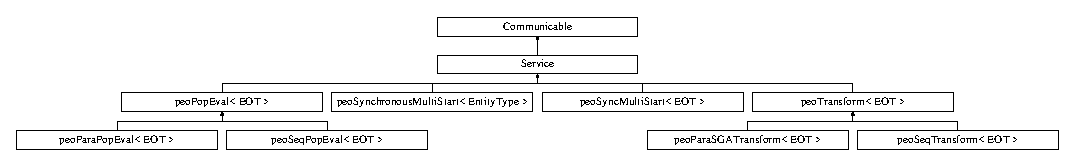
\includegraphics[height=3cm]{classService}
\end{center}
\end{figure}
\subsection*{Public Member Functions}
\begin{CompactItemize}
\item 
\hypertarget{classService_33b149b98498c0e7e401b0f0839d7f0d}{
void \hyperlink{classService_33b149b98498c0e7e401b0f0839d7f0d}{set\-Owner} (\hyperlink{classThread}{Thread} \&\_\-\_\-owner)}
\label{classService_33b149b98498c0e7e401b0f0839d7f0d}

\item 
\hypertarget{classService_0dae00309c51a7b7069788142aed799f}{
\hyperlink{classThread}{Thread} $\ast$ \hyperlink{classService_0dae00309c51a7b7069788142aed799f}{get\-Owner} ()}
\label{classService_0dae00309c51a7b7069788142aed799f}

\item 
\hypertarget{classService_7e2ae35a9070a05dcd46488df649896d}{
void \hyperlink{classService_7e2ae35a9070a05dcd46488df649896d}{request\-Resource\-Request} (unsigned \_\-\_\-how\_\-many=1)}
\label{classService_7e2ae35a9070a05dcd46488df649896d}

\item 
\hypertarget{classService_c4289f98d1cd9ed53e850efbb6a947bd}{
void \hyperlink{classService_c4289f98d1cd9ed53e850efbb6a947bd}{pack\-Resource\-Request} ()}
\label{classService_c4289f98d1cd9ed53e850efbb6a947bd}

\item 
\hypertarget{classService_aea4b8f7f8fb88e83862ee4bfd9ab207}{
virtual void \hyperlink{classService_aea4b8f7f8fb88e83862ee4bfd9ab207}{pack\-Data} ()}
\label{classService_aea4b8f7f8fb88e83862ee4bfd9ab207}

\item 
\hypertarget{classService_3bd87b444710813d30fd754d4d0b4df3}{
virtual void \hyperlink{classService_3bd87b444710813d30fd754d4d0b4df3}{unpack\-Data} ()}
\label{classService_3bd87b444710813d30fd754d4d0b4df3}

\item 
\hypertarget{classService_e4f2894e6121e60f38d41cfbd7447ae4}{
virtual void \hyperlink{classService_e4f2894e6121e60f38d41cfbd7447ae4}{execute} ()}
\label{classService_e4f2894e6121e60f38d41cfbd7447ae4}

\item 
\hypertarget{classService_e5e4f90b2315e15c2a2913bd370f4cf5}{
virtual void \hyperlink{classService_e5e4f90b2315e15c2a2913bd370f4cf5}{pack\-Result} ()}
\label{classService_e5e4f90b2315e15c2a2913bd370f4cf5}

\item 
\hypertarget{classService_45c06344edbfa482b91f68e2035a6099}{
virtual void \hyperlink{classService_45c06344edbfa482b91f68e2035a6099}{unpack\-Result} ()}
\label{classService_45c06344edbfa482b91f68e2035a6099}

\item 
\hypertarget{classService_81ad4d6ebb50045b8977e2ab74826f30}{
virtual void \hyperlink{classService_81ad4d6ebb50045b8977e2ab74826f30}{notify\-Sending\-Data} ()}
\label{classService_81ad4d6ebb50045b8977e2ab74826f30}

\item 
\hypertarget{classService_94e2012e76aaae3aa8199250f558d503}{
virtual void \hyperlink{classService_94e2012e76aaae3aa8199250f558d503}{notify\-Sending\-Resource\-Request} ()}
\label{classService_94e2012e76aaae3aa8199250f558d503}

\item 
\hypertarget{classService_f94cc8a5c2665d4574041737e61e9ffc}{
virtual void \hyperlink{classService_f94cc8a5c2665d4574041737e61e9ffc}{notify\-Sending\-All\-Resource\-Requests} ()}
\label{classService_f94cc8a5c2665d4574041737e61e9ffc}

\end{CompactItemize}
\subsection*{Private Attributes}
\begin{CompactItemize}
\item 
\hypertarget{classService_8b615c65c876f342fe8209eb7e36d7b2}{
\hyperlink{classThread}{Thread} $\ast$ \hyperlink{classService_8b615c65c876f342fe8209eb7e36d7b2}{owner}}
\label{classService_8b615c65c876f342fe8209eb7e36d7b2}

\item 
\hypertarget{classService_a5b2ad9520bb3710b54348b99acebd58}{
unsigned \hyperlink{classService_a5b2ad9520bb3710b54348b99acebd58}{num\_\-sent\_\-rr}}
\label{classService_a5b2ad9520bb3710b54348b99acebd58}

\end{CompactItemize}


\subsection{Detailed Description}




Definition at line 46 of file service.h.

The documentation for this class was generated from the following files:\begin{CompactItemize}
\item 
service.h\item 
core/service.cpp\item 
rmc/mpi/service.cpp\end{CompactItemize}

\hypertarget{classThread}{
\section{Thread Class Reference}
\label{classThread}\index{Thread@{Thread}}
}
Inheritance diagram for Thread::\begin{figure}[H]
\begin{center}
\leavevmode
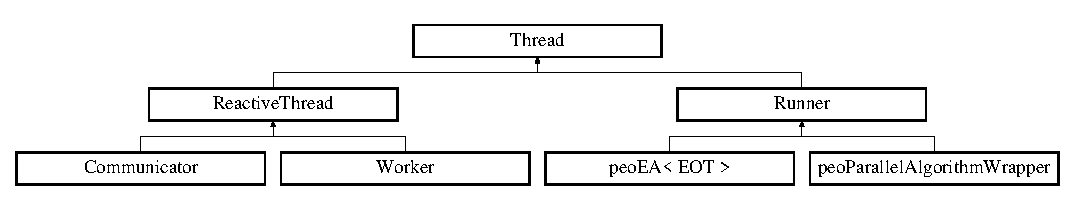
\includegraphics[height=2.25806cm]{classThread}
\end{center}
\end{figure}
\subsection*{Public Member Functions}
\begin{CompactItemize}
\item 
\hypertarget{classThread_95c703fb8f2f27cb64f475a8c940864a}{
\hyperlink{classThread_95c703fb8f2f27cb64f475a8c940864a}{Thread} ()}
\label{classThread_95c703fb8f2f27cb64f475a8c940864a}

\item 
\hypertarget{classThread_37d9edd3a1a776cbc27dedff949c9726}{
virtual \hyperlink{classThread_37d9edd3a1a776cbc27dedff949c9726}{$\sim$Thread} ()}
\label{classThread_37d9edd3a1a776cbc27dedff949c9726}

\item 
\hypertarget{classThread_e197c46f8f62ecce6d2a7fe95bdc5b38}{
void \hyperlink{classThread_e197c46f8f62ecce6d2a7fe95bdc5b38}{set\-Active} ()}
\label{classThread_e197c46f8f62ecce6d2a7fe95bdc5b38}

\item 
\hypertarget{classThread_20632ffe9ddfa2a478afb0c84dc1096b}{
void \hyperlink{classThread_20632ffe9ddfa2a478afb0c84dc1096b}{set\-Passive} ()}
\label{classThread_20632ffe9ddfa2a478afb0c84dc1096b}

\end{CompactItemize}
\subsection*{Private Attributes}
\begin{CompactItemize}
\item 
\hypertarget{classThread_1b155d63bca3096ac4a1d039aea83c7c}{
bool \hyperlink{classThread_1b155d63bca3096ac4a1d039aea83c7c}{act}}
\label{classThread_1b155d63bca3096ac4a1d039aea83c7c}

\end{CompactItemize}


\subsection{Detailed Description}




Definition at line 44 of file thread.h.

The documentation for this class was generated from the following files:\begin{CompactItemize}
\item 
thread.h\item 
thread.cpp\end{CompactItemize}

\hypertarget{classTopology}{
\section{Topology Class Reference}
\label{classTopology}\index{Topology@{Topology}}
}
Inheritance diagram for Topology::\begin{figure}[H]
\begin{center}
\leavevmode
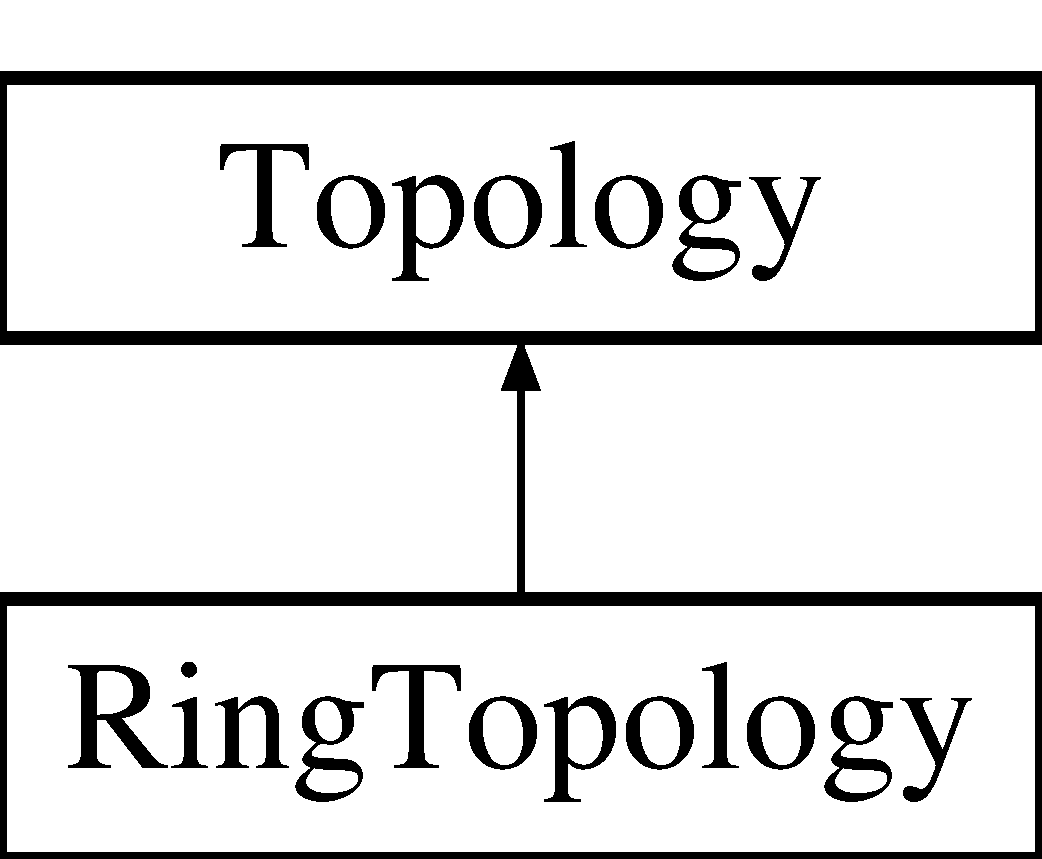
\includegraphics[height=2cm]{classTopology}
\end{center}
\end{figure}
\subsection*{Public Member Functions}
\begin{CompactItemize}
\item 
\hypertarget{classTopology_3e447669757c8311c7f6f8edc705abf2}{
virtual \hyperlink{classTopology_3e447669757c8311c7f6f8edc705abf2}{$\sim$Topology} ()}
\label{classTopology_3e447669757c8311c7f6f8edc705abf2}

\item 
\hypertarget{classTopology_62bc46d8c20fdc71dad9e7c7a0d7aded}{
void \hyperlink{classTopology_62bc46d8c20fdc71dad9e7c7a0d7aded}{add} (\hyperlink{classCooperative}{Cooperative} \&\_\-\_\-mig)}
\label{classTopology_62bc46d8c20fdc71dad9e7c7a0d7aded}

\end{CompactItemize}
\subsection*{Protected Attributes}
\begin{CompactItemize}
\item 
\hypertarget{classTopology_247a2faa8568b678f0b7b11e62c7812c}{
std::vector$<$ \hyperlink{classCooperative}{Cooperative} $\ast$ $>$ \hyperlink{classTopology_247a2faa8568b678f0b7b11e62c7812c}{mig}}
\label{classTopology_247a2faa8568b678f0b7b11e62c7812c}

\end{CompactItemize}


\subsection{Detailed Description}




Definition at line 44 of file topology.h.

The documentation for this class was generated from the following files:\begin{CompactItemize}
\item 
topology.h\item 
topology.cpp\end{CompactItemize}

\hypertarget{classWorker}{
\section{Worker Class Reference}
\label{classWorker}\index{Worker@{Worker}}
}
Inheritance diagram for Worker::\begin{figure}[H]
\begin{center}
\leavevmode
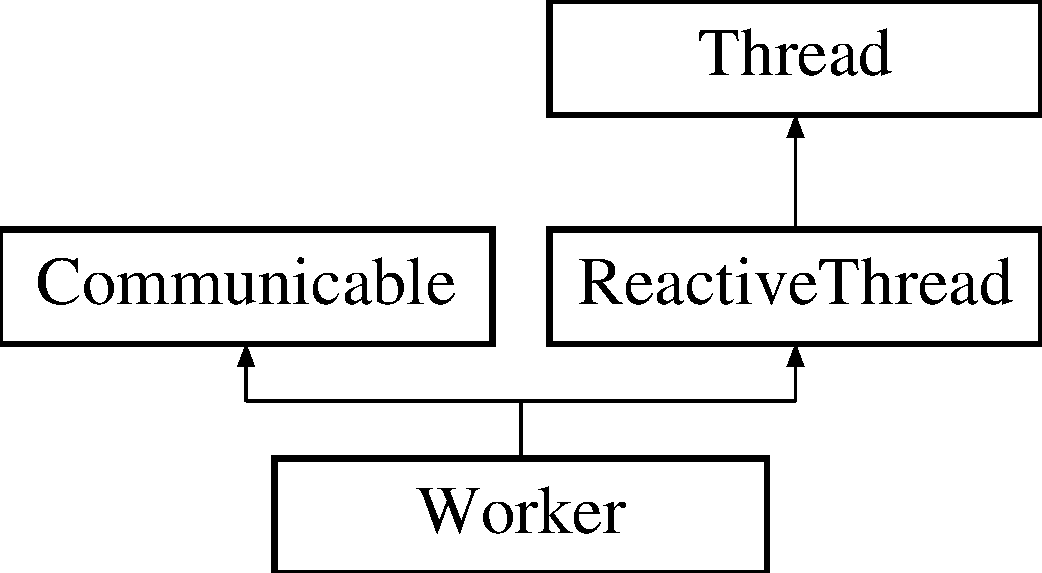
\includegraphics[height=3cm]{classWorker}
\end{center}
\end{figure}
\subsection*{Public Member Functions}
\begin{CompactItemize}
\item 
\hypertarget{classWorker_3754817df06ffe220f7f0d903c78ccac}{
\hyperlink{classWorker_3754817df06ffe220f7f0d903c78ccac}{Worker} ()}
\label{classWorker_3754817df06ffe220f7f0d903c78ccac}

\item 
\hypertarget{classWorker_abcbbace05c6113f1959c494b3577291}{
void \hyperlink{classWorker_abcbbace05c6113f1959c494b3577291}{start} ()}
\label{classWorker_abcbbace05c6113f1959c494b3577291}

\item 
\hypertarget{classWorker_83780920118e6c2b67d9477bdf8be248}{
void \hyperlink{classWorker_83780920118e6c2b67d9477bdf8be248}{pack\-Result} ()}
\label{classWorker_83780920118e6c2b67d9477bdf8be248}

\item 
\hypertarget{classWorker_bff2bdcd64fe5400156cc78704c64953}{
void \hyperlink{classWorker_bff2bdcd64fe5400156cc78704c64953}{unpack\-Data} ()}
\label{classWorker_bff2bdcd64fe5400156cc78704c64953}

\item 
\hypertarget{classWorker_60d2e8eba85b9ef403d94be54c391640}{
void \hyperlink{classWorker_60d2e8eba85b9ef403d94be54c391640}{pack\-Task\-Done} ()}
\label{classWorker_60d2e8eba85b9ef403d94be54c391640}

\item 
\hypertarget{classWorker_e2f487014766a73c5788bdcfd58ad863}{
void \hyperlink{classWorker_e2f487014766a73c5788bdcfd58ad863}{notify\-Sending\-Result} ()}
\label{classWorker_e2f487014766a73c5788bdcfd58ad863}

\item 
\hypertarget{classWorker_13efd6a8e275745329a4a8e23a0eb0bb}{
void \hyperlink{classWorker_13efd6a8e275745329a4a8e23a0eb0bb}{notify\-Sending\-Task\-Done} ()}
\label{classWorker_13efd6a8e275745329a4a8e23a0eb0bb}

\item 
\hypertarget{classWorker_5dab4ea663546b5a49d9398d7a624d27}{
void \hyperlink{classWorker_5dab4ea663546b5a49d9398d7a624d27}{set\-Source} (int \_\-\_\-rank)}
\label{classWorker_5dab4ea663546b5a49d9398d7a624d27}

\end{CompactItemize}
\subsection*{Private Attributes}
\begin{CompactItemize}
\item 
\hypertarget{classWorker_b5ffcb995e12fa71b9551e91729d6972}{
WORKER\_\-ID \hyperlink{classWorker_b5ffcb995e12fa71b9551e91729d6972}{id}}
\label{classWorker_b5ffcb995e12fa71b9551e91729d6972}

\item 
\hypertarget{classWorker_d7dc76e301fd2bcf5d3a2088a59f1378}{
SERVICE\_\-ID \hyperlink{classWorker_d7dc76e301fd2bcf5d3a2088a59f1378}{serv\_\-id}}
\label{classWorker_d7dc76e301fd2bcf5d3a2088a59f1378}

\item 
\hypertarget{classWorker_454e1764ed165af733cc44a73e395692}{
\hyperlink{classService}{Service} $\ast$ \hyperlink{classWorker_454e1764ed165af733cc44a73e395692}{serv}}
\label{classWorker_454e1764ed165af733cc44a73e395692}

\item 
\hypertarget{classWorker_895c3ebc198018ea3391c09bc802d2f6}{
int \hyperlink{classWorker_895c3ebc198018ea3391c09bc802d2f6}{src}}
\label{classWorker_895c3ebc198018ea3391c09bc802d2f6}

\item 
\hypertarget{classWorker_7ba5a18b2918cf9e704536b763be37f7}{
bool \hyperlink{classWorker_7ba5a18b2918cf9e704536b763be37f7}{toto}}
\label{classWorker_7ba5a18b2918cf9e704536b763be37f7}

\end{CompactItemize}


\subsection{Detailed Description}




Definition at line 46 of file worker.h.

The documentation for this class was generated from the following files:\begin{CompactItemize}
\item 
worker.h\item 
worker.cpp\end{CompactItemize}

\printindex
\end{document}
